\documentclass[11pt]{article}
\usepackage[margin=0.9in]{geometry}
\usepackage{booktabs,amsmath,float,graphicx,longtable,array}
\usepackage[T1]{fontenc}\usepackage{lmodern}
\usepackage[colorlinks=true,linkcolor=black,urlcolor=black]{hyperref}
\providecommand{\citep}[1]{}\providecommand{\cite}[1]{}
\title{Note B with the real version as the baseline: results for the sign-off\\ \large Two-year yield, federal funds rate and FCI; nominal and real}
\author{Generated by \texttt{baseline\_real/07*\_report*.py} (FS\_QA FS-A85)}
\date{18 November 2026}
\begin{document}\maketitle
\renewcommand{\ref}[1]{(see table)}

\section*{Specification}
Each number is the response of the unemployment gap (percentage points) or the core PCE price level (percent) to a policy surprise that raises the two-year Treasury yield 1 percentage point in the announcement window. The daily block has the two-year yield, the federal funds rate and, where included, the FCI, all in the same version (nominal, or real: less expected inflation). On the announcement day the funds rate moves by 0.72 per +1 pp on the two-year yield (current-month fed funds futures, MP1). Monthly equations: unemployment gap and core PCE inflation, 12 lags (6 in the appendix), no trend, March--December 2020 dropped, from 1996 or from 1973. Shocks: the 252 Nakamura--Steinsson announcements of 1996--2026. Intervals: 500 draws of the block bootstrap; $^{**}$ and $^{*}$ mark the 5 and 10 percent levels.

\section{Baselines}
\begin{figure}[H]\centering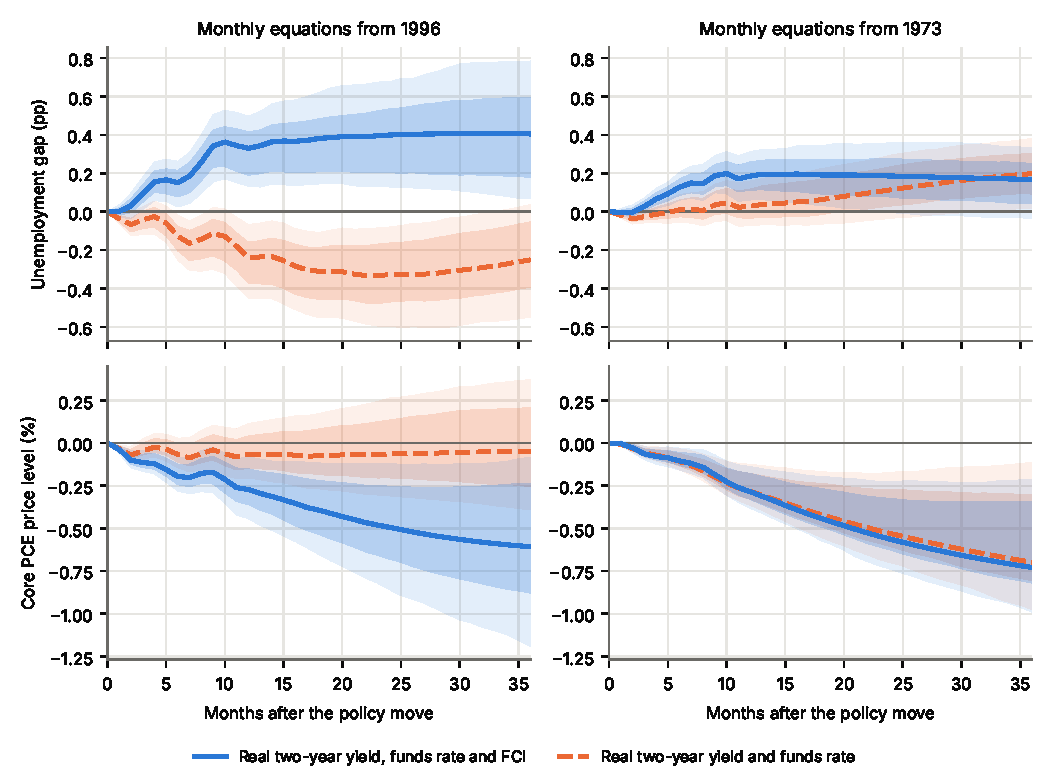
\includegraphics[width=0.95\textwidth]{fig_intro.pdf}\caption{Real baseline, rates alone and with the FCI, from 1996 and from 1973}\end{figure}
\begin{figure}[H]\centering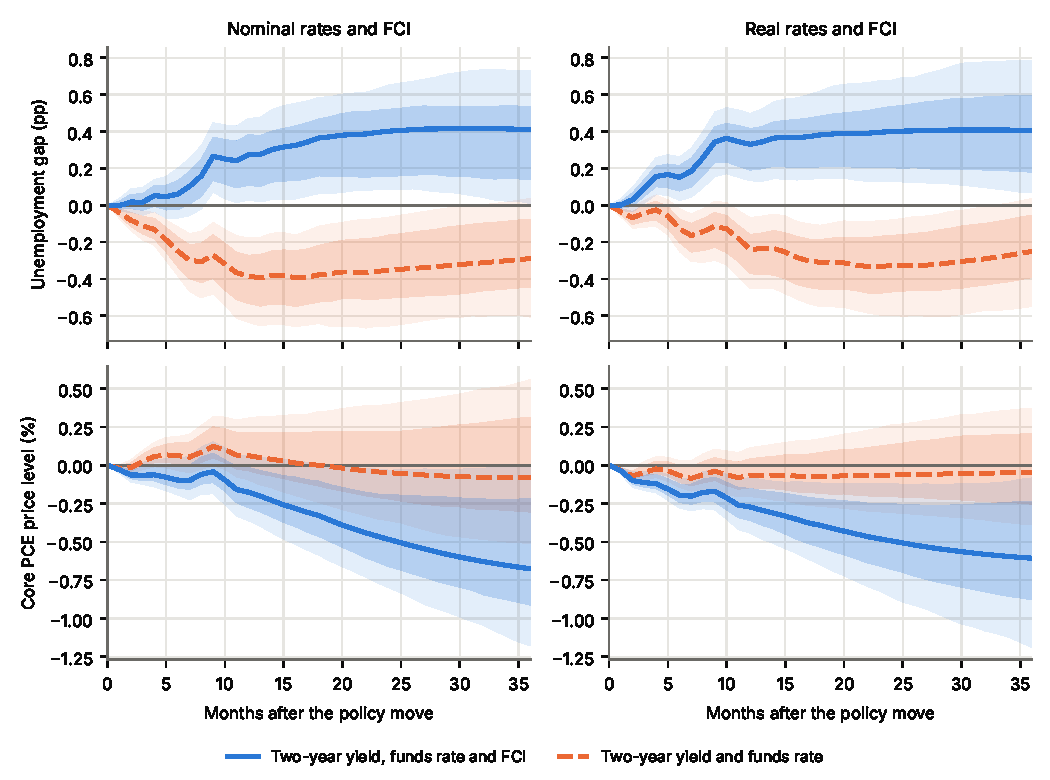
\includegraphics[width=0.95\textwidth]{fig_steps.pdf}\caption{Nominal and real, from 1996}\end{figure}
\begin{figure}[H]\centering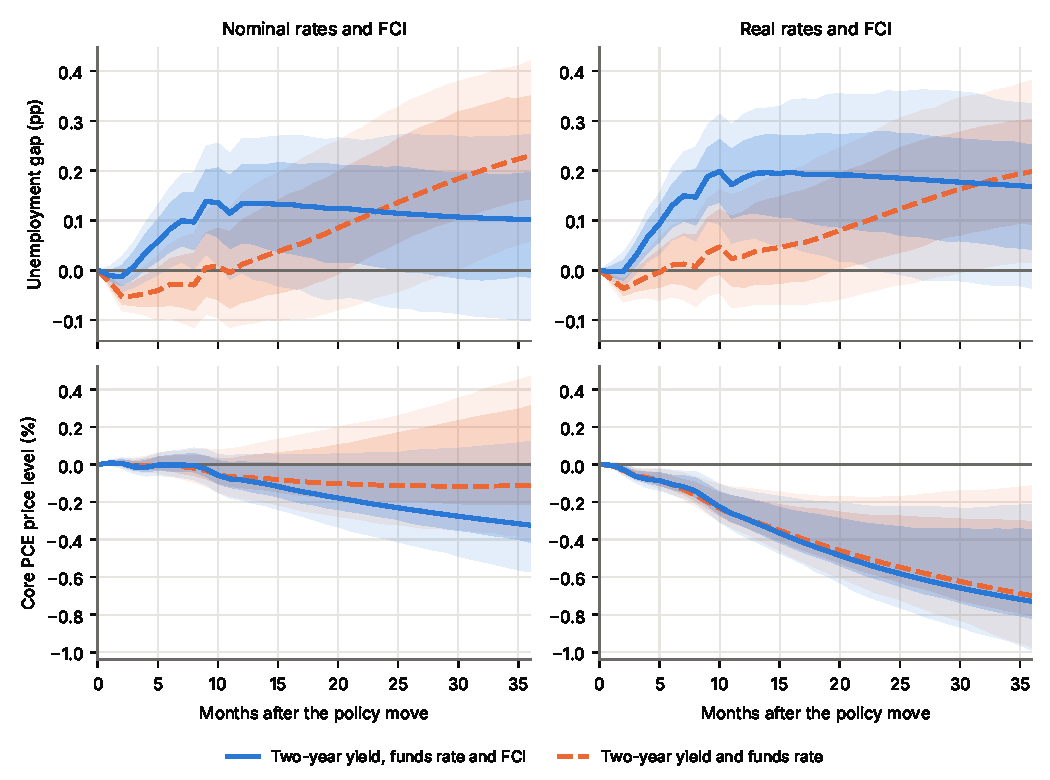
\includegraphics[width=0.95\textwidth]{fig_steps73.pdf}\caption{Nominal and real, from 1973}\end{figure}
\begin{table}[tp]\centering\footnotesize\setlength{\tabcolsep}{2.2pt}
\caption{Baselines: Monthly Equations from 1996 and from 1973, March-December 2020 Dropped (12 Lags)}\label{tab:mainB}
\resizebox{\ifdim\width>\textwidth\textwidth\else\width\fi}{!}{%
\begin{tabular}{llcrrrrrrr}\toprule
 & & & & \multicolumn{3}{c}{Unemployment gap (pp)} & \multicolumn{3}{c}{Price level (\%)}\\ \cmidrule(lr){5-7}\cmidrule(lr){8-10}
Case & FCI & Lags & Obs & 12 m & 24 m & 36 m & 12 m & 24 m & 36 m\\ \midrule
Baseline, 1996: Nominal & none & 12 & 359 & $-$0.38$^{**}$ & $-$0.35$^{**}$ & $-$0.29$^{**}$ & 0.06 & $-$0.05 & $-$0.08\\
 & & & & {\scriptsize [$-$0.63, $-$0.17]} & {\scriptsize [$-$0.71, $-$0.10]} & {\scriptsize [$-$0.81, $-$0.06]} & {\scriptsize [$-$0.13, 0.25]} & {\scriptsize [$-$0.46, 0.32]} & {\scriptsize [$-$0.71, 0.38]}\\
 & nominal & 12 & 359 & 0.27$^{**}$ & 0.40$^{**}$ & 0.41$^{**}$ & $-$0.18 & $-$0.49$^{**}$ & $-$0.68$^{**}$\\
 & & & & {\scriptsize [0.08, 0.53]} & {\scriptsize [0.16, 0.82]} & {\scriptsize [0.20, 1.19]} & {\scriptsize [$-$0.39, 0.04]} & {\scriptsize [$-$0.94, $-$0.13]} & {\scriptsize [$-$1.63, $-$0.24]}\\
\addlinespace
Baseline, 1996: Real & none & 12 & 359 & $-$0.24$^{*}$ & $-$0.33$^{**}$ & $-$0.25$^{**}$ & $-$0.07 & $-$0.06 & $-$0.05\\
 & & & & {\scriptsize [$-$0.42, $-$0.04]} & {\scriptsize [$-$0.63, $-$0.11]} & {\scriptsize [$-$0.73, $-$0.05]} & {\scriptsize [$-$0.25, 0.07]} & {\scriptsize [$-$0.35, 0.21]} & {\scriptsize [$-$0.41, 0.34]}\\
 & real & 12 & 359 & 0.33$^{**}$ & 0.40$^{**}$ & 0.41$^{**}$ & $-$0.27$^{**}$ & $-$0.49$^{**}$ & $-$0.61$^{**}$\\
 & & & & {\scriptsize [0.16, 0.56]} & {\scriptsize [0.18, 0.78]} & {\scriptsize [0.15, 0.96]} & {\scriptsize [$-$0.48, $-$0.13]} & {\scriptsize [$-$0.93, $-$0.17]} & {\scriptsize [$-$1.39, $-$0.17]}\\
\addlinespace
Baseline, 1973: Nominal & none & 12 & 623 & 0.01 & 0.13 & 0.23 & $-$0.07 & $-$0.11 & $-$0.11\\
 & & & & {\scriptsize [$-$0.11, 0.15]} & {\scriptsize [$-$0.09, 0.28]} & {\scriptsize [$-$0.02, 0.39]} & {\scriptsize [$-$0.23, 0.04]} & {\scriptsize [$-$0.44, 0.08]} & {\scriptsize [$-$0.62, 0.16]}\\
 & nominal & 12 & 623 & 0.13$^{*}$ & 0.12 & 0.10 & $-$0.08 & $-$0.22$^{**}$ & $-$0.32$^{**}$\\
 & & & & {\scriptsize [0.01, 0.28]} & {\scriptsize [$-$0.05, 0.28]} & {\scriptsize [$-$0.08, 0.30]} & {\scriptsize [$-$0.24, 0.00]} & {\scriptsize [$-$0.58, $-$0.06]} & {\scriptsize [$-$0.97, $-$0.12]}\\
\addlinespace
Baseline, 1973: Real & none & 12 & 623 & 0.03 & 0.11 & 0.20$^{*}$ & $-$0.28$^{**}$ & $-$0.53$^{**}$ & $-$0.70$^{**}$\\
 & & & & {\scriptsize [$-$0.10, 0.14]} & {\scriptsize [$-$0.06, 0.26]} & {\scriptsize [0.01, 0.37]} & {\scriptsize [$-$0.43, $-$0.18]} & {\scriptsize [$-$0.87, $-$0.33]} & {\scriptsize [$-$1.34, $-$0.40]}\\
 & real & 12 & 623 & 0.19$^{**}$ & 0.19$^{**}$ & 0.17$^{**}$ & $-$0.28$^{**}$ & $-$0.56$^{**}$ & $-$0.73$^{**}$\\
 & & & & {\scriptsize [0.07, 0.32]} & {\scriptsize [0.05, 0.40]} & {\scriptsize [0.04, 0.44]} & {\scriptsize [$-$0.42, $-$0.18]} & {\scriptsize [$-$0.94, $-$0.38]} & {\scriptsize [$-$1.43, $-$0.47]}\\
\bottomrule\end{tabular}}
\begin{flushleft}\footnotesize\textit{Notes:} Nominal and real 2-year yield and funds rate; the FCI is the index in the matching form in each case. March-December 2020 dropped from the monthly and daily equations (values still enter as lags). From 1973: monthly series in place of daily data before 1990. Per +1 pp on the 2-year yield in the window unless stated. $^{**}$ and $^{*}$: significant at the 5 and 10 percent levels (the 95\% and 90\% bootstrap intervals exclude zero); 90\% intervals in brackets. Obs = monthly observations in the equations.\end{flushleft}
\end{table}

\begin{table}[tp]\centering\footnotesize\setlength{\tabcolsep}{3pt}
\caption{Responses without and with the FCI after Two Years}\label{tab:matched}
\resizebox{\ifdim\width>\textwidth\textwidth\else\width\fi}{!}{%
\begin{tabular}{lcccc}\toprule
 & \multicolumn{2}{c}{Monthly equations from 1996} & \multicolumn{2}{c}{Monthly equations from 1973}\\ \cmidrule(lr){2-3}\cmidrule(lr){4-5}
Yield measure & Yield alone & Yield and FCI & Yield alone & Yield and FCI\\ \midrule
\multicolumn{5}{l}{\textit{A. Unemployment gap (percentage points)}}\\
Nominal & $-$0.35$^{**}$ & 0.40$^{**}$ & 0.13 & 0.12\\
 & {\scriptsize [$-$0.66, $-$0.06]} & {\scriptsize [0.09, 0.65]} & {\scriptsize [$-$0.05, 0.32]} & {\scriptsize [$-$0.07, 0.27]}\\
\textbf{Real} & \textbf{$-$0.33$^{**}$} & \textbf{0.40$^{**}$} & \textbf{0.11} & \textbf{0.19}\\
 & {\scriptsize [$-$0.60, $-$0.08]} & {\scriptsize [0.13, 0.68]} & {\scriptsize [$-$0.03, 0.29]} & {\scriptsize [0.00, 0.36]}\\
\addlinespace
\multicolumn{5}{l}{\textit{B. Core PCE price level (percent)}}\\
Nominal & $-$0.05 & $-$0.49$^{*}$ & $-$0.11 & $-$0.22\\
 & {\scriptsize [$-$0.36, 0.40]} & {\scriptsize [$-$0.80, $-$0.03]} & {\scriptsize [$-$0.32, 0.24]} & {\scriptsize [$-$0.40, 0.06]}\\
\textbf{Real} & \textbf{$-$0.06} & \textbf{$-$0.49$^{**}$} & \textbf{$-$0.53$^{**}$} & \textbf{$-$0.56$^{**}$}\\
 & {\scriptsize [$-$0.31, 0.26]} & {\scriptsize [$-$0.86, $-$0.12]} & {\scriptsize [$-$0.70, $-$0.17]} & {\scriptsize [$-$0.74, $-$0.23]}\\
\bottomrule\end{tabular}}
\begin{flushleft}\footnotesize\textit{Notes:} Responses 24 months after a policy move that raises the two-year yield 1 pp in the announcement window; 12 lags; March--December 2020 dropped; the shocks are the 252 announcements of 1996--2026 in both samples. Brackets: 90\% intervals; $^{**}$, $^{*}$: 5 and 10 percent levels. Paired differences (from 1996) are in Appendix Table~\ref{tab:matcheddiff}; 12 and 36 months and other lag lengths in Appendix Tables~\ref{tab:mainB} and~\ref{tab:lags}.\end{flushleft}
\end{table}

\begin{table}[tp]\centering\footnotesize\setlength{\tabcolsep}{3pt}
\caption{Responses without and with the FCI after Two Years, 1996--2026, with Paired Differences}\label{tab:matcheddiff}
\resizebox{\ifdim\width>\textwidth\textwidth\else\width\fi}{!}{%
\begin{tabular}{lcccccc}\toprule
 & \multicolumn{3}{c}{Unemployment gap (pp)} & \multicolumn{3}{c}{Price level (\%)}\\ \cmidrule(lr){2-4}\cmidrule(lr){5-7}
Yield measure & Yield alone & Yield and FCI & Difference & Yield alone & Yield and FCI & Difference\\ \midrule
Nominal & $-$0.35$^{**}$ & 0.40$^{**}$ & 0.75$^{**}$ & $-$0.05 & $-$0.49$^{*}$ & $-$0.44$^{*}$\\
 & {\scriptsize [$-$0.66, $-$0.06]} & {\scriptsize [0.09, 0.65]} & {\scriptsize [0.40, 1.05]} & {\scriptsize [$-$0.36, 0.40]} & {\scriptsize [$-$0.80, $-$0.03]} & {\scriptsize [$-$0.88, $-$0.04]}\\
\addlinespace
Real & $-$0.33$^{**}$ & 0.40$^{**}$ & 0.73$^{**}$ & $-$0.06 & $-$0.49$^{**}$ & $-$0.43$^{**}$\\
 & {\scriptsize [$-$0.60, $-$0.08]} & {\scriptsize [0.13, 0.68]} & {\scriptsize [0.37, 1.04]} & {\scriptsize [$-$0.31, 0.26]} & {\scriptsize [$-$0.86, $-$0.12]} & {\scriptsize [$-$0.82, $-$0.09]}\\
\bottomrule\end{tabular}}
\begin{flushleft}\footnotesize\textit{Notes:} Responses 24 months after a policy move that raises the two-year yield 1 pp in the window, 1996--2026, 12 lags. Differences are computed on common bootstrap draws before rounding. Brackets: 90\% intervals; $^{**}$, $^{*}$: 5 and 10 percent levels. Responses at 12 and 36 months and at 3 and 6 lags are in Appendix Tables~\ref{tab:mainB} and~\ref{tab:lags}.\end{flushleft}
\end{table}

\begin{figure}[H]\centering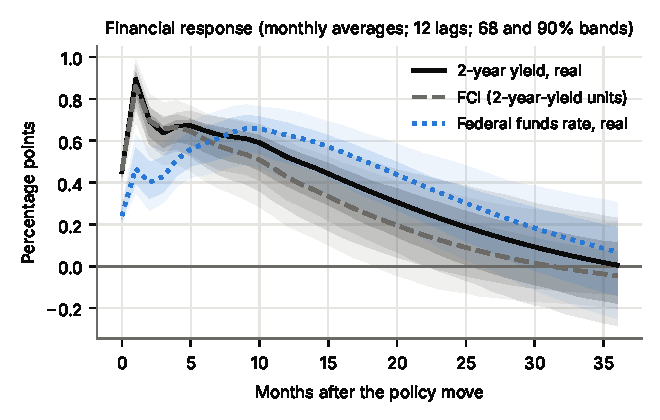
\includegraphics[width=0.62\textwidth]{fig_financial.pdf}\caption{The financial response behind the real baseline}\end{figure}

\section{Standard methods and monthly VARs}
\begin{table}[tp]\centering\small
\caption{Standard Methods: Responses to a 1 Percentage Point Rise in the Two-Year Yield}\label{tab:standard}
\resizebox{\ifdim\width>\textwidth\textwidth\else\width\fi}{!}{%
\begin{tabular}{llcc}\toprule Method & Response & 1996--2026 & 1973--2026\\ \midrule
Recursive (Cholesky) VAR & Unemployment gap, 12 m & $-$0.53$^{*}$ & 0.12\\
 & & {\scriptsize [$-$0.87, $-$0.21]} & {\scriptsize [$-$0.06, 0.35]}\\
 & Unemployment gap, 24 m & $-$0.75$^{*}$ & 0.17\\
 & & {\scriptsize [$-$1.59, $-$0.40]} & {\scriptsize [$-$0.04, 0.41]}\\
 & Price level, 24 m & 0.08 & $-$0.08\\
 & & {\scriptsize [$-$0.50, 0.67]} & {\scriptsize [$-$0.50, 0.29]}\\
 & Price level, 36 m & 0.10 & $-$0.16\\
 & & {\scriptsize [$-$0.63, 1.00]} & {\scriptsize [$-$0.72, 0.47]}\\
\addlinespace
Proxy VAR & Unemployment gap, 12 m & $-$0.41$^{*}$ & $-$0.30\\
 & & {\scriptsize [$-$1.10, $-$0.09]} & {\scriptsize [$-$2.01, 0.13]}\\
 & Unemployment gap, 24 m & $-$0.50$^{*}$ & $-$0.19\\
 & & {\scriptsize [$-$1.17, $-$0.20]} & {\scriptsize [$-$1.48, 0.14]}\\
 & Price level, 24 m & 0.11 & 0.14\\
 & & {\scriptsize [$-$0.61, 0.97]} & {\scriptsize [$-$1.41, 2.32]}\\
 & Price level, 36 m & 0.13 & 0.21\\
 & & {\scriptsize [$-$0.68, 1.09]} & {\scriptsize [$-$1.81, 3.17]}\\
\bottomrule\end{tabular}}
\begin{flushleft}\footnotesize\textit{Notes:} Monthly VARs in the unemployment gap, core PCE inflation and the monthly average of the nominal two-year yield; 12 lags, constant, no trend, March--December 2020 dropped. Cholesky: the yield ordered last, per +1 pp innovation in the yield. Proxy VAR: Nakamura--Steinsson policy news summed within the month as instrument (first-stage $F$ = 5.6 from 1996, 3.8 from 1973), per +1 pp on the yield in the announcement window. Brackets: 90\% intervals (block bootstrap for the Cholesky VARs; exact Anderson--Rubin sets for the proxy VAR). $^{*}$ = excludes zero.\end{flushleft}
\end{table}

\begin{table}[tp]\centering\small
\caption{Monthly VARs with the FCI and the Main Model (Real Two-Year Yield, FCI and Funds Rate; 12 Lags)}\label{tab:monthlycompact}
\resizebox{\ifdim\width>\textwidth\textwidth\else\width\fi}{!}{%
\begin{tabular}{lrrrr}\toprule & \multicolumn{2}{c}{Unemployment gap (pp)} & \multicolumn{2}{c}{Price level (\%)}\\ \cmidrule(lr){2-3}\cmidrule(lr){4-5} & 12 m & 24 m & 12 m & 24 m\\ \midrule
Proxy VAR & $-$0.08 & $-$0.11 & $-$0.47 & $-$0.65\\
 & {\scriptsize [$-$inf, inf]} & {\scriptsize [$-$inf, inf]} & {\scriptsize [$-$inf, inf]} & {\scriptsize [$-$inf, inf]}\\
Window-impact VAR & 0.17$^{*}$ & 0.16$^{*}$ & $-$0.14$^{*}$ & $-$0.23$^{*}$\\
 & {\scriptsize [0.05, 0.38]} & {\scriptsize [0.03, 0.51]} & {\scriptsize [$-$0.28, $-$0.02]} & {\scriptsize [$-$0.47, $-$0.04]}\\
Main model (daily block) & 0.33$^{*}$ & 0.40$^{*}$ & $-$0.27$^{*}$ & $-$0.49$^{*}$\\
 & {\scriptsize [0.16, 0.56]} & {\scriptsize [0.18, 0.78]} & {\scriptsize [$-$0.48, $-$0.13]} & {\scriptsize [$-$0.93, $-$0.17]}\\
\bottomrule\end{tabular}}
\begin{flushleft}\footnotesize\textit{Notes:} Per +1 pp on the two-year yield. $^{*}$: the 90\% interval excludes zero; intervals in brackets (Anderson--Rubin sets for the proxy VAR; bootstrap for the others). Monthly VARs use monthly averages; unit +1 pp on the two-year yield in the announcement window.\end{flushleft}
\end{table}

\begin{table}[tp]\centering\scriptsize\setlength{\tabcolsep}{2pt}
\caption{Monthly VAR Benchmark from 1996 (12 Lags)}\label{tab:mainmonthly}
\resizebox{\ifdim\width>\textwidth\textwidth\else\width\fi}{!}{%
\begin{tabular}{lllcrrrrrrr}\toprule
 & & & & & \multicolumn{3}{c}{Unemployment gap (pp)} & \multicolumn{3}{c}{Price level (\%)}\\ \cmidrule(lr){6-8}\cmidrule(lr){9-11}
2-year & FCI & Identification & Lags & Obs & 12 m & 24 m & 36 m & 12 m & 24 m & 36 m\\
\midrule
Nominal & none & Proxy VAR & 12 & 359 & $-$0.43$^{*}$ & $-$0.48$^{*}$ & $-$0.29$^{*}$ & 0.13 & 0.22 & 0.28\\
 & & & & & {\tiny [$-$1.33, $-$0.11]} & {\tiny [$-$1.19, $-$0.17]} & {\tiny [$-$0.77, $-$0.04]} & {\tiny [$-$0.36, 0.68]} & {\tiny [$-$0.44, 1.14]} & {\tiny [$-$0.47, 1.37]}\\
 &  & Window impact & 12 & 359 & $-$0.28$^{*}$ & $-$0.35$^{*}$ & $-$0.21 & 0.07 & 0.10 & 0.13\\
 & & & & & {\tiny [$-$0.43, $-$0.12]} & {\tiny [$-$0.57, $-$0.05]} & {\tiny [$-$0.42, 0.14]} & {\tiny [$-$0.05, 0.21]} & {\tiny [$-$0.15, 0.39]} & {\tiny [$-$0.24, 0.54]}\\
 & nominal & Proxy VAR & 12 & 359 & $-$0.24 & $-$0.19 & $-$0.01 & $-$0.08 & $-$0.06 & $-$0.03\\
 & & & & & {\tiny unbounded} & {\tiny unbounded} & {\tiny unbounded} & {\tiny unbounded} & {\tiny unbounded} & {\tiny unbounded}\\
 &  & Window impact & 12 & 359 & 0.05 & 0.08 & 0.15 & $-$0.07 & $-$0.13 & $-$0.15\\
 & & & & & {\tiny [$-$0.10, 0.20]} & {\tiny [$-$0.15, 0.29]} & {\tiny [$-$0.10, 0.34]} & {\tiny [$-$0.20, 0.07]} & {\tiny [$-$0.37, 0.10]} & {\tiny [$-$0.45, 0.16]}\\
\addlinespace
Real & none & Proxy VAR & 12 & 359 & $-$0.39$^{*}$ & $-$0.44$^{*}$ & $-$0.30 & $-$0.12 & $-$0.13 & $-$0.13\\
 & & & & & {\tiny [$-$1.55, $-$0.01]} & {\tiny [$-$1.47, $-$0.04]} & {\tiny [$-$1.05, 0.02]} & {\tiny [$-$0.77, 0.48]} & {\tiny [$-$1.01, 0.79]} & {\tiny [$-$1.14, 0.90]}\\
 &  & Window impact & 12 & 359 & $-$0.14 & $-$0.19 & $-$0.09 & $-$0.04 & $-$0.05 & $-$0.03\\
 & & & & & {\tiny [$-$0.25, 0.01]} & {\tiny [$-$0.35, 0.04]} & {\tiny [$-$0.25, 0.16]} & {\tiny [$-$0.16, 0.08]} & {\tiny [$-$0.28, 0.18]} & {\tiny [$-$0.35, 0.25]}\\
 & real & Proxy VAR & 12 & 359 & $-$0.08 & $-$0.11 & $-$0.06 & $-$0.47 & $-$0.65 & $-$0.72\\
 & & & & & {\tiny unbounded} & {\tiny unbounded} & {\tiny unbounded} & {\tiny unbounded} & {\tiny unbounded} & {\tiny unbounded}\\
 &  & Window impact & 12 & 359 & 0.17 & 0.16 & 0.17 & $-$0.14 & $-$0.23 & $-$0.25\\
 & & & & & {\tiny [$-$0.01, 0.29]} & {\tiny [$-$0.07, 0.35]} & {\tiny [$-$0.07, 0.35]} & {\tiny [$-$0.26, 0.00]} & {\tiny [$-$0.43, 0.01]} & {\tiny [$-$0.53, 0.05]}\\
\bottomrule\end{tabular}}
\begin{flushleft}\footnotesize\textit{Notes:} Monthly VAR in the unemployment gap, core PCE inflation, the monthly averages of the 2-year yield, of the FCI when included, and of the federal funds rate (same version), to September 2026, no trend, March--December 2020 dropped. Proxy VAR: Nakamura--Steinsson surprise as instrument; sets are exact 90\% Anderson--Rubin sets, ``unbounded'' when the instrument cannot reject large effects. Window impact: impact vector taken from the daily model (the month-average response to a window surprise); 90\% bootstrap intervals. Unit in both: +1 pp on the 2-year yield in the announcement window.\end{flushleft}
\end{table}

\begin{table}[tp]\centering\scriptsize\setlength{\tabcolsep}{2pt}
\caption{Monthly VAR Benchmark from 1973 (12 Lags)}\label{tab:mainmonthly73}
\resizebox{\ifdim\width>\textwidth\textwidth\else\width\fi}{!}{%
\begin{tabular}{lllcrrrrrrr}\toprule
 & & & & & \multicolumn{3}{c}{Unemployment gap (pp)} & \multicolumn{3}{c}{Price level (\%)}\\ \cmidrule(lr){6-8}\cmidrule(lr){9-11}
2-year & FCI & Identification & Lags & Obs & 12 m & 24 m & 36 m & 12 m & 24 m & 36 m\\
\midrule
Nominal & none & Proxy VAR & 12 & 623 & $-$0.32 & $-$0.25 & $-$0.13 & 0.06 & 0.12 & 0.17\\
 & & & & & {\tiny [$-$1.95, 0.09]} & {\tiny [$-$1.48, 0.08]} & {\tiny [$-$0.75, 0.07]} & {\tiny [$-$0.81, 1.47]} & {\tiny [$-$1.25, 2.62]} & {\tiny [$-$1.62, 3.55]}\\
 &  & Window impact & 12 & 623 & 0.01 & 0.03 & 0.03 & $-$0.03 & $-$0.07 & $-$0.11\\
 & & & & & {\tiny [$-$0.07, 0.11]} & {\tiny [$-$0.09, 0.13]} & {\tiny [$-$0.07, 0.13]} & {\tiny [$-$0.11, 0.06]} & {\tiny [$-$0.26, 0.08]} & {\tiny [$-$0.44, 0.11]}\\
 & nominal & Proxy VAR & 12 & 623 & $-$0.49 & $-$0.58 & $-$0.48 & $-$0.03 & $-$0.14 & $-$0.17\\
 & & & & & {\tiny unbounded} & {\tiny unbounded} & {\tiny unbounded} & {\tiny unbounded} & {\tiny unbounded} & {\tiny unbounded}\\
 &  & Window impact & 12 & 623 & 0.21$^{*}$ & 0.17$^{*}$ & 0.09$^{*}$ & $-$0.03 & $-$0.12 & $-$0.17\\
 & & & & & {\tiny [0.10, 0.33]} & {\tiny [0.07, 0.32]} & {\tiny [0.00, 0.22]} & {\tiny [$-$0.13, 0.08]} & {\tiny [$-$0.34, 0.08]} & {\tiny [$-$0.53, 0.10]}\\
\addlinespace
Real & none & Proxy VAR & 12 & 623 & $-$0.31 & $-$0.25 & $-$0.14 & $-$0.04 & $-$0.08 & $-$0.11\\
 & & & & & {\tiny [$-$4.97, 0.20]} & {\tiny [$-$3.50, 0.21]} & {\tiny [$-$1.62, 0.20]} & {\tiny [$-$1.33, 2.83]} & {\tiny [$-$2.07, 5.23]} & {\tiny [$-$2.69, 6.99]}\\
 &  & Window impact & 12 & 623 & 0.03 & 0.02 & 0.00 & $-$0.16$^{*}$ & $-$0.34$^{*}$ & $-$0.47$^{*}$\\
 & & & & & {\tiny [$-$0.06, 0.11]} & {\tiny [$-$0.10, 0.12]} & {\tiny [$-$0.12, 0.10]} & {\tiny [$-$0.27, $-$0.11]} & {\tiny [$-$0.64, $-$0.24]} & {\tiny [$-$0.91, $-$0.31]}\\
 & real & Proxy VAR & 12 & 623 & $-$0.36 & $-$0.41 & $-$0.34 & $-$0.04 & $-$0.18 & $-$0.24\\
 & & & & & {\tiny unbounded} & {\tiny unbounded} & {\tiny unbounded} & {\tiny unbounded} & {\tiny unbounded} & {\tiny unbounded}\\
 &  & Window impact & 12 & 623 & 0.23$^{*}$ & 0.19$^{*}$ & 0.08 & $-$0.15$^{*}$ & $-$0.35$^{*}$ & $-$0.46$^{*}$\\
 & & & & & {\tiny [0.13, 0.36]} & {\tiny [0.08, 0.34]} & {\tiny [$-$0.02, 0.26]} & {\tiny [$-$0.27, $-$0.06]} & {\tiny [$-$0.65, $-$0.19]} & {\tiny [$-$0.92, $-$0.24]}\\
\bottomrule\end{tabular}}
\begin{flushleft}\footnotesize\textit{Notes:} Monthly VAR in the unemployment gap, core PCE inflation, the monthly averages of the 2-year yield, of the FCI when included, and of the federal funds rate (same version), to September 2026, no trend, March--December 2020 dropped. Proxy VAR: Nakamura--Steinsson surprise as instrument; sets are exact 90\% Anderson--Rubin sets, ``unbounded'' when the instrument cannot reject large effects. Window impact: impact vector taken from the daily model (the month-average response to a window surprise); 90\% bootstrap intervals. Unit in both: +1 pp on the 2-year yield in the announcement window.\end{flushleft}
\end{table}

\begin{table}[tp]\centering\small
\caption{Monthly Proxy VAR: First-Stage Strength and Impact on the FCI}\label{tab:monthlyF}
\resizebox{\ifdim\width>\textwidth\textwidth\else\width\fi}{!}{%
\begin{tabular}{llrrrr}\toprule 2-year & FCI & $F$ (6 lags) & $F$ (12) & Proxy impact on FCI & Model impact on FCI\\ \midrule
\multicolumn{6}{l}{\textit{Monthly equations from 1996}}\\
Nominal & none & 4.9 & 5.3 &  & \\
 & nominal & 2.0 & 1.4 & 0.18 & 1.10\\
Real & none & 5.2 & 5.1 &  & \\
 & real & 2.9 & 1.6 & 0.33 & 1.02\\
\multicolumn{6}{l}{\textit{Monthly equations from 1973}}\\
Nominal & none & 4.7 & 3.8 &  & \\
 & nominal & 0.7 & 0.2 & 0.29 & 1.10\\
Real & none & 3.8 & 3.2 &  & \\
 & real & 0.3 & 0.2 & 0.12 & 1.02\\
\bottomrule\end{tabular}}
\begin{flushleft}\footnotesize\textit{Notes:} $F$: robust first-stage statistic of the policy-variable residual on the instrument (instrument months only, 1996--2026; monthly equations from 1996 or from 1973). Impact on FCI: response of the month's average FCI per +1 pp on the month's average 2-year yield, estimated from monthly residuals (proxy VAR, 12 lags) and implied by the daily model.\end{flushleft}
\end{table}

\begin{table}[tp]\centering\small
\caption{A Monthly Proxy VAR when the Real Model is the True Process}\label{tab:proxysim}
\resizebox{\ifdim\width>\textwidth\textwidth\else\width\fi}{!}{%
\begin{tabular}{lrrrr}\toprule Estimate & Data & True & Simulated median & 5th--95th percentile\\ \midrule
\multicolumn{5}{l}{\textit{A. Proxy VAR with the FCI}}\\
\quad First-stage $F$ & 1.6 &  & 3.3 & [0.1, 13.7]\\
\quad Unemployment gap, 12 m & $-$0.08 & 0.33 & 0.17 & [$-$0.54, 1.46]\\
\quad Price level, 24 m & $-$0.65 & $-$0.49 & $-$0.25 & [$-$1.75, 0.81]\\
\multicolumn{5}{l}{\textit{B. Proxy VAR without the FCI}}\\
\quad Unemployment gap, 12 m & $-$0.39 & 0.33 & $-$0.07 & [$-$0.92, 0.81]\\
\multicolumn{5}{l}{\textit{C. Monthly VAR with the window impact and the FCI}}\\
\quad Unemployment gap, 12 m & 0.17 & 0.33 & 0.18 & [0.04, 0.32]\\
\bottomrule\end{tabular}}
\begin{flushleft}\footnotesize\textit{Notes:} 1,000 samples of 369 months generated by the estimated real model with the FCI and the funds rate (12 lags), with the data's calendar and announcement days; policy reaches unemployment and prices only through the 2-year yield, the FCI and the funds rate. Data: the 1996 sample, 12 lags, real measures, March--December 2020 dropped; monthly averages in the monthly VAR. True: the model's response per +1 pp on the 2-year yield in the announcement window (the unit of every panel). Simulated: median and 5th--95th percentiles of the estimates.\end{flushleft}
\end{table}


\section{The sacrifice ratio}
\begin{table}[tp]\centering\footnotesize\setlength{\tabcolsep}{3pt}
\caption{Implied Trade-Off: The Phillips Multiplier}\label{tab:tradeoff}
\resizebox{\ifdim\width>\textwidth\textwidth\else\width\fi}{!}{%
\begin{tabular}{lcccc}\toprule
 & \multicolumn{2}{c}{24 months} & \multicolumn{2}{c}{36 months}\\ \cmidrule(lr){2-3}\cmidrule(lr){4-5}
Rates and FCI, measured as & Estimate & 90\% set & Estimate & 90\% set\\ \midrule
Nominal, 1996 start & $-$1.02 & [$-$3.74, $-$0.09] & $-$0.76 & [$-$2.46, 0.03]\\
\textbf{Real, 1996 start (baseline)} & \textbf{$-$0.85} & \textbf{[$-$1.61, $-$0.26]} & \textbf{$-$0.61} & \textbf{[$-$1.23, $-$0.11]}\\
Nominal, 1973 start & $-$1.11 & undefined; 68\%: [$-$2.48, $-$0.08] & $-$1.05 & undefined; 68\%: [$-$2.96, 0.00]\\
Real, 1973 start & $-$1.85 & [$-$5.36, $-$0.77] & $-$1.52 & [$-$5.82, $-$0.49]\\
\bottomrule\end{tabular}}
\begin{flushleft}\footnotesize\textit{Notes:} $\kappa_H$ is the core PCE price level at month $H$ (percent) per percentage-point year of cumulative unemployment-gap response \citep{barnichon2021}; its inverse in absolute value is the sacrifice ratio. Estimate: ratio of the point responses. 90\% set: Anderson--Rubin type, all values for which the 90\% bootstrap interval of $\tilde P_H-\kappa\tilde U_H$ contains zero. The ratio is undefined when the 90\% interval of the cumulative unemployment response includes zero, because the data then cannot rule out unemployment responses of zero or either sign; the 68\% set is then shown where it exists. 12 lags. All cases in Appendix Table~\ref{tab:tradefull}.\end{flushleft}
\end{table}

\begin{table}[tp]\centering\small
\caption{Implied Trade-Off: Phillips Multiplier $\kappa_H$ (12 Lags), All Cases}\label{tab:tradefull}
\resizebox{\ifdim\width>\textwidth\textwidth\else\width\fi}{!}{%
\begin{tabular}{llrrrr}\toprule & & \multicolumn{2}{c}{Multiplier $\kappa_H$} & \multicolumn{2}{c}{Cost (sacrifice ratio)}\\ \cmidrule(lr){3-4}\cmidrule(lr){5-6} Case & FCI & $H=24$ & $H=36$ & $H=24$ & $H=36$\\ \midrule
\multicolumn{6}{l}{\textit{Baseline, 1996}}\\
Nominal & none & 0.08 [$-$0.36, 1.38] & 0.09 [$-$0.29, 1.48] & not defined & not defined\\
 & nominal & $-$1.02 [$-$2.38, $-$0.29]$^{\dagger}$ & $-$0.76 [$-$1.64, $-$0.29] & 0.98 [0.42, 3.49] & 1.32 [0.61, 3.41]$^{\dagger}$\\
Real & none & 0.16 [$-$0.45, 2.27] & 0.07 [$-$0.42, 1.44] & not defined & not defined\\
 & real & $-$0.85 [$-$1.45, $-$0.33] & $-$0.61 [$-$1.08, $-$0.18] & 1.18 [0.69, 3.03] & 1.63 [0.93, 5.41]\\
\addlinespace
\multicolumn{6}{l}{\textit{Baseline, 1973}}\\
Nominal & none & $-$2.32 (undefined; 68\%: undefined) & $-$0.48 (undefined; 68\%: undefined) & 0.43 (unbounded) & 2.08 (unbounded)\\
 & nominal & $-$1.11 (undefined; 68\%: [$-$3.57, $-$0.64]) & $-$1.05 (undefined; 68\%: [$-$4.06, $-$0.72]) & 0.90 [$-$0.06, 3.09] & 0.95 [$-$0.10, 2.65]\\
Real & none & $-$6.94 (undefined; 68\%: undefined) & $-$2.90 (undefined; 68\%: undefined) & 0.14 [$-$0.34, 0.47] & 0.34 [$-$0.23, 0.82]\\
 & real & $-$1.85 [$-$5.37, $-$1.16] & $-$1.52 [$-$4.92, $-$0.92] & 0.54 [0.19, 0.86] & 0.66 [0.20, 1.09]\\
\addlinespace
\multicolumn{6}{l}{\textit{Robustness tests and the final section, real with the FCI}}\\
2020 left in, 1996 & real & $-$1.21 (undefined; 68\%: [$-$2.80, $-$0.73]) & $-$0.93 (undefined; 68\%: [$-$1.95, $-$0.58]) & 0.83 [$-$0.08, 1.90] & 1.07 [$-$0.02, 2.71]\\
2020 left in, 1973 & real & $-$13.29 (undefined; 68\%: undefined) & $-$5.84 (undefined; 68\%: undefined) & 0.08 [$-$0.74, 0.75] & 0.17 [$-$0.78, 1.35]\\
IP added, 1996 & real & $-$0.90 [$-$1.61, $-$0.41] & $-$0.60 [$-$1.08, $-$0.20] & 1.12 [0.62, 2.44] & 1.67 [0.92, 5.12]\\
IP added, 1973 & real & $-$0.80 [$-$1.48, $-$0.52] & $-$0.50 [$-$0.98, $-$0.23] & 1.25 [0.68, 1.92] & 1.98 [1.02, 4.41]\\
Bauer-Swanson surprise, 1996 & real & $-$0.80 [$-$1.34, $-$0.33] & $-$0.59 [$-$1.00, $-$0.19] & 1.24 [0.74, 3.04] & 1.71 [1.00, 5.29]\\
Bauer-Swanson surprise, 1973 & real & $-$1.57 [$-$3.29, $-$1.01] & $-$1.30 [$-$3.17, $-$0.76] & 0.64 [0.30, 0.99] & 0.77 [0.32, 1.31]\\
Without the funds rate, 1996 & real & $-$1.16 [$-$7.10, $-$0.30] & $-$0.90 [$-$228.66, $-$0.11] & 0.86 [0.14, 3.38] & 1.11 [0.00, 9.33]$^{\dagger}$\\
Without the funds rate, 1973 & real & $-$1.56 [$-$3.24, $-$0.95] & $-$1.89 [$-$5.30, $-$1.00] & 0.64 [0.31, 1.05] & 0.53 [0.19, 1.00]\\
Monthly equations from 1985 & real & $-$0.64 [$-$3.79, 10.49]$^{\dagger}$ & $-$0.26 (undefined; 68\%: [$-$1.06, 0.24]) & 1.57 (unbounded) & 3.85 (unbounded)\\
Cubic spline trend, 1996 & real & $-$0.44 [$-$1.05, 0.65] & $-$0.22 [$-$0.69, 0.83] & 2.25 (unbounded) & 4.47 (unbounded)\\
Cubic spline trend, 1973 & real & $-$1.06 [$-$2.26, $-$0.61] & $-$0.74 [$-$1.59, $-$0.42] & 0.94 [0.44, 1.63] & 1.34 [0.63, 2.38]\\
Ends 2019, 1996 & real & 0.42 (undefined; 68\%: [0.13, 1.32]) & 0.31 (undefined; 68\%: [0.06, 11.18]) & not defined & not defined\\
Ends 2019, 1973 & real & $-$1.32 [$-$12.76, $-$0.64] & $-$1.30 [$-$73.92, $-$0.51] & 0.76 [0.08, 1.57] & 0.77 [0.01, 1.95]\\
r*-gap (LW), 1996 & r*-gap & $-$1.06 [$-$1.73, $-$0.69] & $-$0.83 [$-$1.59, $-$0.49] & 0.94 [0.58, 1.44] & 1.21 [0.63, 2.03]\\
r*-gap (LW), 1973 & r*-gap & $-$1.32 [$-$3.02, $-$0.92] & $-$1.03 [$-$2.86, $-$0.71] & 0.76 [0.33, 1.09] & 0.97 [0.35, 1.41]\\
\addlinespace
Real minus nominal, with FCI & & [$-$0.97, 1.96] & [$-$0.78, 1.67] & & \\
\bottomrule\end{tabular}}
\begin{flushleft}\footnotesize\textit{Notes:} $\kappa_H$ = core PCE price level at month $H$ (percent) per percentage-point year of cumulative unemployment-gap response (Barnichon and Mesters 2021); the sacrifice ratio is $-1/\kappa_H$. Point estimate and 90\% confidence set (Anderson--Rubin type) in brackets, computed exactly (a wide grid refined by bisection), so a finite end is never an artifact of the grid. An infinite end means that the 90\% interval of the cumulative unemployment response includes zero: the data then cannot rule out arbitrarily steep trade-offs on that side; ``unbounded'': both sides. $^{\dagger}$: the set has a gap wider than 2 percent of its width; shown is its hull. Ends 2019: all equations end in December 2019 (2020 not dropped). Cost: percentage-point years of cumulative unemployment per 1 percent lower price level, with the 90\% set obtained by inverting the test for the cost itself (bounded whenever the price response is well estimated; ``not defined'' where the price level does not fall). Last row: paired difference over common announcement draws.\end{flushleft}
\end{table}


\section{How much do policy shocks explain?}
\begin{figure}[H]\centering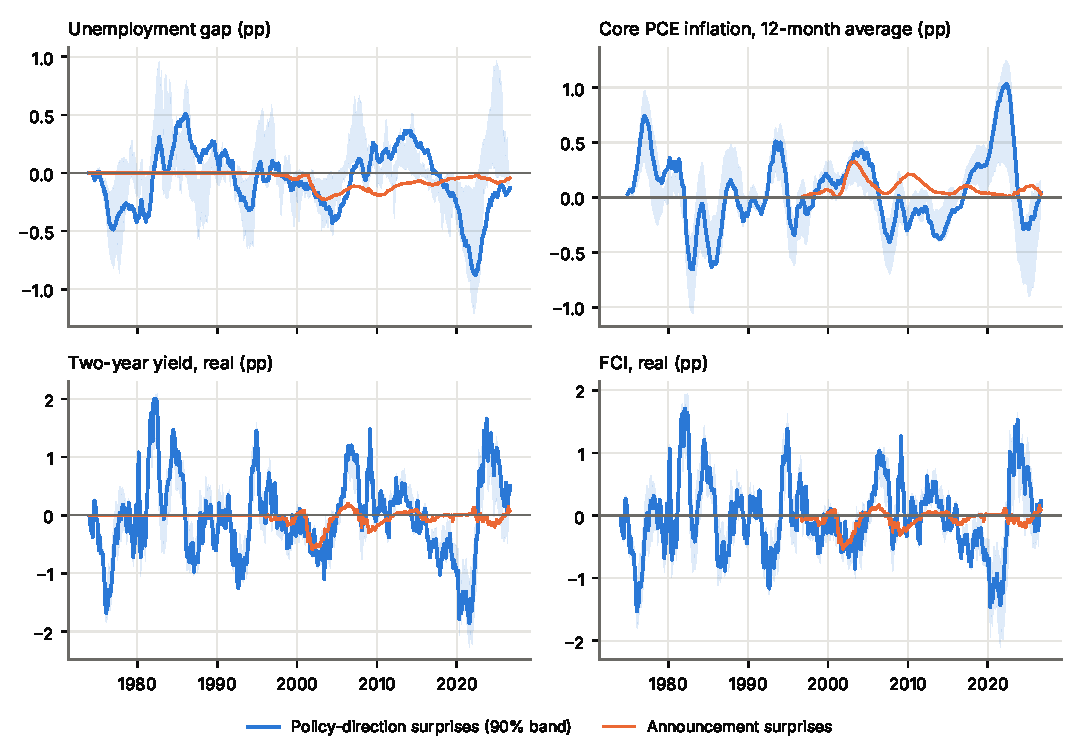
\includegraphics[width=0.95\textwidth]{fig_decomp_hd.pdf}\caption{Historical contributions of policy-direction shocks (real model from 1973)}\end{figure}
\begin{table}[tp]\centering\small
\caption{How Much Policy Shocks Explain: Variance Shares at 24 Months}\label{tab:decompshares}
\resizebox{\ifdim\width>\textwidth\textwidth\else\width\fi}{!}{%
\begin{tabular}{lcccc}\toprule & \multicolumn{2}{c}{Model from 1996} & \multicolumn{2}{c}{Model from 1973}\\ \cmidrule(lr){2-3}\cmidrule(lr){4-5} Shocks & Unemployment gap & Core inflation & Unemployment gap & Core inflation\\ \midrule
Measured window surprises, 1996--2026 & 0.7 & 0.3 & 0.2 & 0.2\\
 & {\scriptsize [0.1, 1.6]} & {\scriptsize [0.1, 0.6]} & {\scriptsize [0.0, 0.5]} & {\scriptsize [0.1, 0.4]}\\
Policy-direction shocks, 1990--2026 & 11.6 & 5.7 & 3.2 & 4.1\\
 & {\scriptsize [2.1, 29.7]} & {\scriptsize [2.5, 11.6]} & {\scriptsize [0.5, 9.1]} & {\scriptsize [1.4, 7.2]}\\
\quad of which on days without an announcement & 12.6 & 5.7 & 3.5 & 4.5\\
 & {\scriptsize [2.2, 32.1]} & {\scriptsize [2.4, 12.1]} & {\scriptsize [0.5, 9.8]} & {\scriptsize [1.4, 7.8]}\\
Policy-direction shocks, 1974--1989 & 12.2 & 4.3 & 3.4 & 3.6\\
 & {\scriptsize [2.4, 31.0]} & {\scriptsize [2.6, 10.5]} & {\scriptsize [0.5, 9.6]} & {\scriptsize [1.3, 6.6]}\\
\bottomrule\end{tabular}}
\begin{flushleft}\footnotesize\textit{Notes:} Percent of the 24-month forecast-error variance (monthly VAR in monthly averages from 1973, 12 lags) accounted for by the contributions of the shocks of the last 24 months, propagated through the real model with the FCI and the funds rate (12 lags, March--December 2020 dropped) with monthly equations from 1996 or from 1973; shares over the stated period, March--December 2020 excluded. Measured window surprises: the 252 announcements. Policy-direction shocks: the daily movement of the two-year yield and the FCI in the direction of the window response, recovered from the daily block on every day from 1990; before 1990 from the monthly VAR, scaled to the daily shocks' size. Brackets: 90\% bootstrap bands of Note B's responses.\end{flushleft}
\end{table}


\section{Mechanisms}
\begin{table}[tp]\centering\small
\caption{Two Corrections: Announcement Timing and Financial Conditions (24 Months; 12 Lags)}\label{tab:timing2}
\resizebox{\ifdim\width>\textwidth\textwidth\else\width\fi}{!}{%
\begin{tabular}{llcccc}\toprule & & \multicolumn{2}{c}{Yield alone} & \multicolumn{2}{c}{Yield and FCI}\\ \cmidrule(lr){3-4}\cmidrule(lr){5-6}
Yield & Response & Monthly VAR & Daily block & Monthly VAR & Daily block\\ \midrule
Nominal & Unemployment gap (pp) & $-$0.35$^{*}$ & $-$0.35$^{**}$ & 0.08 & 0.40$^{**}$\\
 & Price level (\%) & 0.10 & $-$0.05 & $-$0.13 & $-$0.49$^{*}$\\\addlinespace
Real & Unemployment gap (pp) & $-$0.19 & $-$0.33$^{**}$ & 0.16 & 0.40$^{**}$\\
 & Price level (\%) & $-$0.05 & $-$0.06 & $-$0.23 & $-$0.49$^{**}$\\
\bottomrule\end{tabular}}
\begin{flushleft}\footnotesize\textit{Notes:} Per +1 pp on the two-year yield in the announcement window, 1996--2026. Monthly VAR: the window-impact monthly VAR of Section~\ref{sec:monthlyvar}, which takes the impact from the windows and treats every announcement as if it fell at the start of its month (end-of-month series). Daily block: the main model, which tracks when in the month each announcement falls. $^{**}$ and $^{*}$: the 95 and 90 percent intervals exclude zero.\end{flushleft}
\end{table}

\begin{table}[tp]\centering\small
\caption{Credit, Activity and the Effect of Adding the FCI (Real Rates; 24 Months)}\label{tab:credit}
\resizebox{\ifdim\width>\textwidth\textwidth\else\width\fi}{!}{%
\begin{tabular}{lcccc}\toprule & \multicolumn{2}{c}{Unemployment gap (pp)} & \multicolumn{2}{c}{Effect of adding the FCI} \\ \cmidrule(lr){2-3}\cmidrule(lr){4-5}
 & Rates alone & Rates and FCI & Unemployment gap & Price level (\%)\\ \midrule
Baseline & $-$0.33$^{*}$ & 0.40$^{*}$ & 0.73$^{*}$ & $-$0.43$^{*}$\\
 & {\scriptsize [$-$0.60, $-$0.08]} & {\scriptsize [0.13, 0.68]} & {\scriptsize [0.37, 1.04]} & {\scriptsize [$-$0.82, $-$0.09]}\\
Baa spread in the daily block & $-$0.22 & 0.27 & 0.49$^{*}$ & $-$0.50$^{*}$\\
 & {\scriptsize [$-$0.58, 0.12]} & {\scriptsize [$-$0.05, 0.55]} & {\scriptsize [0.19, 0.77]} & {\scriptsize [$-$0.80, $-$0.15]}\\
Industrial production in the monthly block & $-$0.07 & 0.52$^{*}$ & 0.59$^{*}$ & $-$0.60$^{*}$\\
 & {\scriptsize [$-$0.38, 0.13]} & {\scriptsize [0.22, 0.86]} & {\scriptsize [0.31, 0.96]} & {\scriptsize [$-$1.01, $-$0.29]}\\
\bottomrule\end{tabular}}
\begin{flushleft}\footnotesize\textit{Notes:} Per +1 pp on the two-year yield in the announcement window; real two-year yield and funds rate, 12 lags, monthly equations from 1996, March--December 2020 dropped. Baa spread: Moody's Baa yield less the 10-year Treasury yield, in the daily block next to the rates (and the FCI); its impact is its announcement-day change on the surprise, because it has no intraday series; months before the daily data (1986) use the monthly series. Industrial production: $100\ln$ of the index, a third monthly variable, set like unemployment and inflation before markets within the month. Effect of adding the FCI: the response with the FCI less the response with the same variables without it. All cases use the same bootstrap draws, so the effects are paired; 90 percent intervals in brackets; $^{*}$: the 90 percent interval excludes zero.\end{flushleft}
\end{table}

\begin{table}[tp]\centering\footnotesize\setlength{\tabcolsep}{3pt}
\caption{Financial Persistence: Direct Estimates and the Model}\label{tab:persist}
\resizebox{\ifdim\width>\textwidth\textwidth\else\width\fi}{!}{%
\begin{tabular}{llccc}\toprule
Series & & Direct estimate & With later announcements controlled & Model\\ \midrule
Two-year yield & Day 5 & 0.82 & 0.80 & 0.97\\
 & & {\scriptsize [0.56, 1.04]} & {\scriptsize [0.55, 1.04]} & {\scriptsize [0.92, 1.01]}\\
 & Day 22 & 0.80 & 0.74 & 0.89\\
 & & {\scriptsize [0.18, 1.23]} & {\scriptsize [0.14, 1.19]} & {\scriptsize [0.76, 0.96]}\\
 & Day 66 & 0.74 & 0.82 & 0.64\\
 & & {\scriptsize [$-$0.25, 1.45]} & {\scriptsize [$-$0.11, 1.60]} & {\scriptsize [0.53, 0.70]}\\
 & Average, days 0--21 & 0.89 & 0.84 & 0.96\\
 & & {\scriptsize [0.53, 1.16]} & {\scriptsize [0.49, 1.12]} & {\scriptsize [0.88, 1.01]}\\
\addlinespace
FCI & Day 5 & 1.37 & 1.40 & 1.02\\
 & & {\scriptsize [1.11, 1.73]} & {\scriptsize [1.13, 1.76]} & {\scriptsize [0.89, 1.15]}\\
 & Day 22 & 1.14 & 1.15 & 0.83\\
 & & {\scriptsize [0.62, 1.70]} & {\scriptsize [0.64, 1.76]} & {\scriptsize [0.66, 0.96]}\\
 & Day 66 & 0.67 & 0.66 & 0.66\\
 & & {\scriptsize [$-$0.10, 1.52]} & {\scriptsize [$-$0.09, 1.60]} & {\scriptsize [0.49, 0.79]}\\
 & Average, days 0--21 & 1.49 & 1.57 & 0.95\\
 & & {\scriptsize [1.22, 1.91]} & {\scriptsize [1.31, 1.94]} & {\scriptsize [0.81, 1.08]}\\
\bottomrule\end{tabular}}
\begin{flushleft}\footnotesize\textit{Notes:} Response per +1 pp on the two-year yield in the window, real versions, 251 announcements with 66 trading days after them. Day 0 is the announcement day; the change on day $h$ is the window move plus the change in the close from day 0 to day $h$, the convention of the model, and the average is over days 0 to 21 (22 trading days). Direct estimate: slope of that change on the policy-news surprise divided by the window slope of the yield; second column adds the surprises of announcements within the horizon. 90\% intervals from 2,000 draws of moving blocks of 12 calendar months with the normalization re-estimated. Model: the baseline of Table~\ref{tab:matched} on weekdays; 90\% bootstrap interval. Close minus window on the announcement day (the window-to-close gap): $-$0.11 [$-$0.32, 0.12] for the yield and $-$0.27 [$-$0.43, $-$0.14] for the FCI, per +1 pp in the window.\end{flushleft}
\end{table}


\section{Robustness}
\begin{table}[tp]\centering\small
\caption{Robustness: Responses at 12 Months}\label{tab:robsummary}
\resizebox{\ifdim\width>\textwidth\textwidth\else\width\fi}{!}{%
\begin{tabular}{lcccc}\toprule & \multicolumn{2}{c}{Monthly equations from 1996} & \multicolumn{2}{c}{Monthly equations from 1973}\\ \cmidrule(lr){2-3}\cmidrule(lr){4-5} & Unemployment gap & Price level & Unemployment gap & Price level\\ \midrule
\multicolumn{5}{l}{\textit{Real 2-year yield, funds rate and FCI}}\\
Baseline & 0.33$^{**}$ & $-$0.27$^{**}$ & 0.19$^{**}$ & $-$0.28$^{**}$\\
 & {\scriptsize [0.13, 0.50]} & {\scriptsize [$-$0.44, $-$0.08]} & {\scriptsize [0.06, 0.31]} & {\scriptsize [$-$0.38, $-$0.14]}\\
2020 left in & 0.24 & $-$0.30$^{**}$ & 0.02 & $-$0.21$^{**}$\\
 & {\scriptsize [$-$0.25, 0.62]} & {\scriptsize [$-$0.50, $-$0.10]} & {\scriptsize [$-$0.16, 0.22]} & {\scriptsize [$-$0.32, $-$0.06]}\\
Excess bond premium and industrial production added & 0.24$^{*}$ & $-$0.30$^{**}$ & 0.13$^{**}$ & $-$0.17$^{**}$\\
 & {\scriptsize [0.02, 0.41]} & {\scriptsize [$-$0.45, $-$0.09]} & {\scriptsize [0.02, 0.26]} & {\scriptsize [$-$0.25, $-$0.04]}\\
Bauer--Swanson surprise & 0.37$^{**}$ & $-$0.29$^{**}$ & 0.22$^{**}$ & $-$0.28$^{**}$\\
 & {\scriptsize [0.16, 0.55]} & {\scriptsize [$-$0.47, $-$0.10]} & {\scriptsize [0.09, 0.35]} & {\scriptsize [$-$0.38, $-$0.13]}\\
6 lags & 0.26$^{**}$ & $-$0.19 & 0.11 & $-$0.18$^{**}$\\
 & {\scriptsize [0.08, 0.40]} & {\scriptsize [$-$0.36, 0.01]} & {\scriptsize [$-$0.01, 0.21]} & {\scriptsize [$-$0.27, $-$0.02]}\\
Without the funds rate & 0.17$^{*}$ & $-$0.22$^{**}$ & 0.25$^{**}$ & $-$0.24$^{**}$\\
 & {\scriptsize [0.01, 0.35]} & {\scriptsize [$-$0.38, $-$0.05]} & {\scriptsize [0.11, 0.35]} & {\scriptsize [$-$0.33, $-$0.11]}\\
Monthly equations from 1985 & 0.12 & $-$0.07 &  & \\
 & {\scriptsize [$-$0.06, 0.23]} & {\scriptsize [$-$0.19, 0.11]} &  & \\
\addlinespace\multicolumn{5}{l}{\textit{Nominal 2-year yield, funds rate and FCI}}\\
Baseline & 0.27$^{*}$ & $-$0.18 & 0.13 & $-$0.08\\
 & {\scriptsize [0.03, 0.47]} & {\scriptsize [$-$0.36, 0.06]} & {\scriptsize [$-$0.01, 0.26]} & {\scriptsize [$-$0.19, 0.05]}\\
2020 left in & 0.35 & $-$0.18 & $-$0.13 & 0.02\\
 & {\scriptsize [$-$0.13, 0.75]} & {\scriptsize [$-$0.40, 0.05]} & {\scriptsize [$-$0.36, 0.06]} & {\scriptsize [$-$0.09, 0.19]}\\
Excess bond premium and industrial production added & 0.39$^{**}$ & $-$0.31$^{**}$ & 0.17$^{**}$ & $-$0.03\\
 & {\scriptsize [0.11, 0.55]} & {\scriptsize [$-$0.48, $-$0.09]} & {\scriptsize [0.06, 0.28]} & {\scriptsize [$-$0.13, 0.10]}\\
Bauer--Swanson surprise & 0.32$^{**}$ & $-$0.19 & 0.17$^{**}$ & $-$0.08\\
 & {\scriptsize [0.05, 0.52]} & {\scriptsize [$-$0.39, 0.06]} & {\scriptsize [0.02, 0.30]} & {\scriptsize [$-$0.19, 0.06]}\\
6 lags & 0.06 & $-$0.17 & 0.04 & $-$0.03\\
 & {\scriptsize [$-$0.14, 0.24]} & {\scriptsize [$-$0.36, 0.05]} & {\scriptsize [$-$0.10, 0.14]} & {\scriptsize [$-$0.13, 0.12]}\\
Without the funds rate & 0.13 & $-$0.14 & 0.29$^{**}$ & $-$0.01\\
 & {\scriptsize [$-$0.04, 0.36]} & {\scriptsize [$-$0.33, 0.07]} & {\scriptsize [0.13, 0.41]} & {\scriptsize [$-$0.13, 0.12]}\\
Monthly equations from 1985 & 0.04 & 0.02 &  & \\
 & {\scriptsize [$-$0.12, 0.16]} & {\scriptsize [$-$0.08, 0.17]} &  & \\
\bottomrule\end{tabular}}
\begin{flushleft}\footnotesize\textit{Notes:} Two-year yield, federal funds rate and FCI in the stated version; responses 12 months after a policy move that raises the two-year yield 1 percentage point in the announcement window; unemployment gap in percentage points, price level in percent; 12 lags unless stated; March--December 2020 dropped unless stated. The 1985 start has monthly equations from January 1985 (1996 columns). $^{**}$ and $^{*}$: the 95\% and 90\% bootstrap intervals exclude zero; 90\% intervals in brackets. Full results at 12, 24 and 36 months for both versions are in the appendix.\end{flushleft}
\end{table}

\begin{table}[tp]\centering\footnotesize\setlength{\tabcolsep}{2.2pt}
\caption{Robustness Tests (12 Lags)}\label{tab:mainR}
\resizebox{\ifdim\width>\textwidth\textwidth\else\width\fi}{!}{%
\begin{tabular}{llcrrrrrrr}\toprule
 & & & & \multicolumn{3}{c}{Unemployment gap (pp)} & \multicolumn{3}{c}{Price level (\%)}\\ \cmidrule(lr){5-7}\cmidrule(lr){8-10}
Case & FCI & Lags & Obs & 12 m & 24 m & 36 m & 12 m & 24 m & 36 m\\ \midrule
2020 left in, 1996: Nominal & none & 12 & 369 & $-$0.62$^{**}$ & $-$0.37 & $-$0.37 & 0.19 & $-$0.05 & $-$0.19\\
 & & & & {\scriptsize [$-$1.17, $-$0.18]} & {\scriptsize [$-$0.84, 0.03]} & {\scriptsize [$-$0.78, 0.05]} & {\scriptsize [$-$0.03, 0.48]} & {\scriptsize [$-$0.47, 0.41]} & {\scriptsize [$-$0.74, 0.40]}\\
 & nominal & 12 & 369 & 0.35 & 0.25 & 0.15 & $-$0.18 & $-$0.59$^{**}$ & $-$0.82$^{**}$\\
 & & & & {\scriptsize [$-$0.12, 0.76]} & {\scriptsize [$-$0.08, 0.81]} & {\scriptsize [$-$0.16, 0.85]} & {\scriptsize [$-$0.42, 0.03]} & {\scriptsize [$-$1.08, $-$0.23]} & {\scriptsize [$-$1.63, $-$0.34]}\\
\addlinespace
2020 left in, 1996: Real & none & 12 & 369 & $-$0.60$^{**}$ & $-$0.37$^{**}$ & $-$0.22 & 0.00 & $-$0.07 & $-$0.17\\
 & & & & {\scriptsize [$-$1.06, $-$0.26]} & {\scriptsize [$-$0.80, $-$0.12]} & {\scriptsize [$-$0.69, 0.06]} & {\scriptsize [$-$0.20, 0.20]} & {\scriptsize [$-$0.41, 0.29]} & {\scriptsize [$-$0.68, 0.36]}\\
 & real & 12 & 369 & 0.24 & 0.30 & 0.26 & $-$0.30$^{**}$ & $-$0.56$^{**}$ & $-$0.70$^{**}$\\
 & & & & {\scriptsize [$-$0.20, 0.66]} & {\scriptsize [$-$0.04, 0.75]} & {\scriptsize [$-$0.08, 0.83]} & {\scriptsize [$-$0.54, $-$0.12]} & {\scriptsize [$-$1.12, $-$0.25]} & {\scriptsize [$-$1.60, $-$0.25]}\\
\addlinespace
2020 left in, 1973: Nominal & none & 12 & 633 & $-$0.37$^{**}$ & $-$0.17$^{**}$ & 0.00 & 0.04 & 0.11 & 0.20\\
 & & & & {\scriptsize [$-$0.62, $-$0.25]} & {\scriptsize [$-$0.64, $-$0.07]} & {\scriptsize [$-$0.37, 0.13]} & {\scriptsize [$-$0.16, 0.15]} & {\scriptsize [$-$0.34, 0.29]} & {\scriptsize [$-$0.71, 0.44]}\\
 & nominal & 12 & 633 & $-$0.13 & $-$0.13 & $-$0.09 & 0.02 & 0.05 & 0.08\\
 & & & & {\scriptsize [$-$0.35, 0.07]} & {\scriptsize [$-$0.39, 0.08]} & {\scriptsize [$-$0.39, 0.13]} & {\scriptsize [$-$0.14, 0.13]} & {\scriptsize [$-$0.31, 0.24]} & {\scriptsize [$-$0.48, 0.36]}\\
\addlinespace
2020 left in, 1973: Real & none & 12 & 633 & $-$0.22$^{**}$ & $-$0.07 & 0.07 & $-$0.20$^{**}$ & $-$0.36$^{**}$ & $-$0.47$^{**}$\\
 & & & & {\scriptsize [$-$0.40, $-$0.10]} & {\scriptsize [$-$0.26, 0.07]} & {\scriptsize [$-$0.14, 0.22]} & {\scriptsize [$-$0.33, $-$0.10]} & {\scriptsize [$-$0.70, $-$0.17]} & {\scriptsize [$-$1.19, $-$0.18]}\\
 & real & 12 & 633 & 0.02 & 0.03 & 0.05 & $-$0.21$^{**}$ & $-$0.37$^{**}$ & $-$0.44$^{**}$\\
 & & & & {\scriptsize [$-$0.16, 0.22]} & {\scriptsize [$-$0.15, 0.25]} & {\scriptsize [$-$0.10, 0.38]} & {\scriptsize [$-$0.36, $-$0.10]} & {\scriptsize [$-$0.70, $-$0.19]} & {\scriptsize [$-$1.04, $-$0.15]}\\
\addlinespace
IP added, 1996: Nominal & none & 12 & 359 & $-$0.29$^{**}$ & $-$0.02 & 0.15 & 0.13 & 0.13 & 0.24\\
 & & & & {\scriptsize [$-$0.49, $-$0.09]} & {\scriptsize [$-$0.26, 0.32]} & {\scriptsize [$-$0.13, 0.63]} & {\scriptsize [$-$0.03, 0.32]} & {\scriptsize [$-$0.17, 0.45]} & {\scriptsize [$-$0.21, 0.81]}\\
 & nominal & 12 & 359 & 0.23$^{**}$ & 0.50$^{**}$ & 0.55$^{**}$ & $-$0.25$^{*}$ & $-$0.55$^{**}$ & $-$0.72$^{*}$\\
 & & & & {\scriptsize [0.03, 0.51]} & {\scriptsize [0.19, 0.94]} & {\scriptsize [0.22, 1.25]} & {\scriptsize [$-$0.45, $-$0.04]} & {\scriptsize [$-$0.92, $-$0.09]} & {\scriptsize [$-$1.38, $-$0.07]}\\
\addlinespace
IP added, 1996: Real & none & 12 & 359 & $-$0.18 & $-$0.07 & 0.18 & 0.00 & 0.05 & 0.09\\
 & & & & {\scriptsize [$-$0.34, 0.04]} & {\scriptsize [$-$0.35, 0.19]} & {\scriptsize [$-$0.10, 0.53]} & {\scriptsize [$-$0.16, 0.14]} & {\scriptsize [$-$0.25, 0.30]} & {\scriptsize [$-$0.32, 0.51]}\\
 & real & 12 & 359 & 0.31$^{**}$ & 0.52$^{**}$ & 0.59$^{**}$ & $-$0.32$^{**}$ & $-$0.55$^{**}$ & $-$0.70$^{**}$\\
 & & & & {\scriptsize [0.16, 0.60]} & {\scriptsize [0.30, 0.95]} & {\scriptsize [0.29, 1.20]} & {\scriptsize [$-$0.53, $-$0.16]} & {\scriptsize [$-$0.96, $-$0.21]} & {\scriptsize [$-$1.39, $-$0.22]}\\
\addlinespace
IP added, 1973: Nominal & none & 12 & 623 & 0.10 & 0.29$^{**}$ & 0.42$^{**}$ & $-$0.07 & $-$0.13 & $-$0.14\\
 & & & & {\scriptsize [$-$0.05, 0.24]} & {\scriptsize [0.13, 0.50]} & {\scriptsize [0.25, 0.67]} & {\scriptsize [$-$0.21, 0.02]} & {\scriptsize [$-$0.40, 0.02]} & {\scriptsize [$-$0.52, 0.06]}\\
 & nominal & 12 & 623 & 0.21$^{**}$ & 0.26$^{**}$ & 0.24$^{**}$ & $-$0.07 & $-$0.15$^{*}$ & $-$0.18$^{*}$\\
 & & & & {\scriptsize [0.09, 0.35]} & {\scriptsize [0.12, 0.45]} & {\scriptsize [0.11, 0.48]} & {\scriptsize [$-$0.22, 0.02]} & {\scriptsize [$-$0.42, $-$0.02]} & {\scriptsize [$-$0.50, 0.00]}\\
\addlinespace
IP added, 1973: Real & none & 12 & 623 & 0.10 & 0.28$^{**}$ & 0.37$^{**}$ & $-$0.22$^{**}$ & $-$0.32$^{**}$ & $-$0.35$^{**}$\\
 & & & & {\scriptsize [$-$0.02, 0.21]} & {\scriptsize [0.12, 0.44]} & {\scriptsize [0.22, 0.62]} & {\scriptsize [$-$0.36, $-$0.14]} & {\scriptsize [$-$0.57, $-$0.18]} & {\scriptsize [$-$0.75, $-$0.15]}\\
 & real & 12 & 623 & 0.25$^{**}$ & 0.30$^{**}$ & 0.24$^{**}$ & $-$0.23$^{**}$ & $-$0.35$^{**}$ & $-$0.36$^{**}$\\
 & & & & {\scriptsize [0.13, 0.41]} & {\scriptsize [0.15, 0.52]} & {\scriptsize [0.09, 0.52]} & {\scriptsize [$-$0.38, $-$0.15]} & {\scriptsize [$-$0.63, $-$0.20]} & {\scriptsize [$-$0.81, $-$0.15]}\\
\addlinespace
Bauer-Swanson surprise, 1996: Nominal & none & 12 & 359 & $-$0.38$^{**}$ & $-$0.35$^{**}$ & $-$0.29$^{**}$ & 0.06 & $-$0.05 & $-$0.08\\
 & & & & {\scriptsize [$-$0.63, $-$0.17]} & {\scriptsize [$-$0.71, $-$0.10]} & {\scriptsize [$-$0.81, $-$0.06]} & {\scriptsize [$-$0.13, 0.25]} & {\scriptsize [$-$0.47, 0.32]} & {\scriptsize [$-$0.71, 0.38]}\\
 & nominal & 12 & 359 & 0.32$^{**}$ & 0.45$^{**}$ & 0.45$^{**}$ & $-$0.19 & $-$0.52$^{**}$ & $-$0.72$^{**}$\\
 & & & & {\scriptsize [0.13, 0.59]} & {\scriptsize [0.23, 1.01]} & {\scriptsize [0.22, 1.28]} & {\scriptsize [$-$0.41, 0.03]} & {\scriptsize [$-$1.01, $-$0.14]} & {\scriptsize [$-$1.80, $-$0.27]}\\
\addlinespace
Bauer-Swanson surprise, 1996: Real & none & 12 & 359 & $-$0.24$^{*}$ & $-$0.33$^{**}$ & $-$0.25$^{**}$ & $-$0.07 & $-$0.06 & $-$0.05\\
 & & & & {\scriptsize [$-$0.42, $-$0.04]} & {\scriptsize [$-$0.63, $-$0.11]} & {\scriptsize [$-$0.73, $-$0.05]} & {\scriptsize [$-$0.25, 0.07]} & {\scriptsize [$-$0.35, 0.21]} & {\scriptsize [$-$0.41, 0.34]}\\
 & real & 12 & 359 & 0.37$^{**}$ & 0.45$^{**}$ & 0.44$^{**}$ & $-$0.29$^{**}$ & $-$0.52$^{**}$ & $-$0.64$^{**}$\\
 & & & & {\scriptsize [0.20, 0.62]} & {\scriptsize [0.21, 0.90]} & {\scriptsize [0.18, 1.07]} & {\scriptsize [$-$0.52, $-$0.14]} & {\scriptsize [$-$1.01, $-$0.20]} & {\scriptsize [$-$1.49, $-$0.18]}\\
\addlinespace
Bauer-Swanson surprise, 1973: Nominal & none & 12 & 623 & 0.01 & 0.13 & 0.23 & $-$0.07 & $-$0.11 & $-$0.11\\
 & & & & {\scriptsize [$-$0.11, 0.15]} & {\scriptsize [$-$0.09, 0.28]} & {\scriptsize [$-$0.02, 0.39]} & {\scriptsize [$-$0.23, 0.04]} & {\scriptsize [$-$0.44, 0.08]} & {\scriptsize [$-$0.62, 0.16]}\\
 & nominal & 12 & 623 & 0.17$^{**}$ & 0.14 & 0.11 & $-$0.08 & $-$0.21$^{**}$ & $-$0.31$^{**}$\\
 & & & & {\scriptsize [0.04, 0.31]} & {\scriptsize [$-$0.01, 0.33]} & {\scriptsize [$-$0.07, 0.32]} & {\scriptsize [$-$0.24, 0.01]} & {\scriptsize [$-$0.60, $-$0.06]} & {\scriptsize [$-$0.96, $-$0.09]}\\
\addlinespace
Bauer-Swanson surprise, 1973: Real & none & 12 & 623 & 0.03 & 0.11 & 0.20$^{*}$ & $-$0.28$^{**}$ & $-$0.53$^{**}$ & $-$0.70$^{**}$\\
 & & & & {\scriptsize [$-$0.10, 0.14]} & {\scriptsize [$-$0.06, 0.26]} & {\scriptsize [0.01, 0.37]} & {\scriptsize [$-$0.43, $-$0.18]} & {\scriptsize [$-$0.87, $-$0.33]} & {\scriptsize [$-$1.34, $-$0.40]}\\
 & real & 12 & 623 & 0.22$^{**}$ & 0.21$^{**}$ & 0.18$^{**}$ & $-$0.28$^{**}$ & $-$0.56$^{**}$ & $-$0.72$^{**}$\\
 & & & & {\scriptsize [0.11, 0.37]} & {\scriptsize [0.08, 0.43]} & {\scriptsize [0.04, 0.47]} & {\scriptsize [$-$0.43, $-$0.18]} & {\scriptsize [$-$0.94, $-$0.38]} & {\scriptsize [$-$1.42, $-$0.47]}\\
\addlinespace
Without the funds rate, 1996: Nominal & none & 12 & 359 & $-$0.37$^{**}$ & $-$0.45$^{**}$ & $-$0.37$^{**}$ & 0.01 & 0.06 & 0.06\\
 & & & & {\scriptsize [$-$0.56, $-$0.19]} & {\scriptsize [$-$0.85, $-$0.26]} & {\scriptsize [$-$0.84, $-$0.16]} & {\scriptsize [$-$0.15, 0.17]} & {\scriptsize [$-$0.22, 0.37]} & {\scriptsize [$-$0.33, 0.56]}\\
 & nominal & 12 & 359 & 0.13 & 0.16 & 0.16 & $-$0.14 & $-$0.29 & $-$0.42\\
 & & & & {\scriptsize [$-$0.07, 0.34]} & {\scriptsize [$-$0.19, 0.41]} & {\scriptsize [$-$0.26, 0.44]} & {\scriptsize [$-$0.33, 0.07]} & {\scriptsize [$-$0.66, 0.14]} & {\scriptsize [$-$0.98, 0.17]}\\
\addlinespace
Without the funds rate, 1996: Real & none & 12 & 359 & $-$0.28$^{**}$ & $-$0.35$^{**}$ & $-$0.30$^{**}$ & $-$0.08 & $-$0.06 & $-$0.06\\
 & & & & {\scriptsize [$-$0.44, $-$0.11]} & {\scriptsize [$-$0.64, $-$0.15]} & {\scriptsize [$-$0.67, $-$0.10]} & {\scriptsize [$-$0.25, 0.03]} & {\scriptsize [$-$0.34, 0.15]} & {\scriptsize [$-$0.41, 0.25]}\\
 & real & 12 & 359 & 0.17$^{*}$ & 0.23 & 0.22 & $-$0.22$^{**}$ & $-$0.38$^{**}$ & $-$0.50$^{*}$\\
 & & & & {\scriptsize [0.02, 0.35]} & {\scriptsize [$-$0.01, 0.48]} & {\scriptsize [$-$0.05, 0.55]} & {\scriptsize [$-$0.40, $-$0.07]} & {\scriptsize [$-$0.76, $-$0.08]} & {\scriptsize [$-$1.04, $-$0.06]}\\
\addlinespace
Without the funds rate, 1973: Nominal & none & 12 & 623 & 0.11$^{*}$ & 0.17$^{**}$ & 0.13$^{**}$ & $-$0.01 & $-$0.08 & $-$0.15\\
 & & & & {\scriptsize [0.00, 0.25]} & {\scriptsize [0.08, 0.37]} & {\scriptsize [0.05, 0.30]} & {\scriptsize [$-$0.15, 0.09]} & {\scriptsize [$-$0.39, 0.11]} & {\scriptsize [$-$0.65, 0.08]}\\
 & nominal & 12 & 623 & 0.29$^{**}$ & 0.19$^{**}$ & 0.06 & $-$0.01 & $-$0.17$^{*}$ & $-$0.33$^{**}$\\
 & & & & {\scriptsize [0.17, 0.45]} & {\scriptsize [0.09, 0.46]} & {\scriptsize [$-$0.06, 0.27]} & {\scriptsize [$-$0.17, 0.08]} & {\scriptsize [$-$0.43, $-$0.01]} & {\scriptsize [$-$0.79, $-$0.16]}\\
\addlinespace
Without the funds rate, 1973: Real & none & 12 & 623 & 0.09 & 0.08 & 0.02 & $-$0.23$^{**}$ & $-$0.49$^{**}$ & $-$0.72$^{**}$\\
 & & & & {\scriptsize [$-$0.01, 0.22]} & {\scriptsize [$-$0.03, 0.23]} & {\scriptsize [$-$0.09, 0.19]} & {\scriptsize [$-$0.35, $-$0.14]} & {\scriptsize [$-$0.78, $-$0.33]} & {\scriptsize [$-$1.32, $-$0.49]}\\
 & real & 12 & 623 & 0.25$^{**}$ & 0.13$^{*}$ & 0.02 & $-$0.24$^{**}$ & $-$0.55$^{**}$ & $-$0.79$^{**}$\\
 & & & & {\scriptsize [0.14, 0.40]} & {\scriptsize [0.01, 0.33]} & {\scriptsize [$-$0.09, 0.25]} & {\scriptsize [$-$0.38, $-$0.15]} & {\scriptsize [$-$0.85, $-$0.40]} & {\scriptsize [$-$1.33, $-$0.59]}\\
\addlinespace
Monthly equations from 1985: Nominal & none & 12 & 491 & $-$0.23$^{**}$ & $-$0.29$^{**}$ & $-$0.23$^{**}$ & 0.06 & 0.15 & 0.28\\
 & & & & {\scriptsize [$-$0.37, $-$0.10]} & {\scriptsize [$-$0.55, $-$0.13]} & {\scriptsize [$-$0.49, $-$0.06]} & {\scriptsize [$-$0.06, 0.19]} & {\scriptsize [$-$0.06, 0.41]} & {\scriptsize [$-$0.03, 0.64]}\\
 & nominal & 12 & 491 & 0.04 & 0.01 & 0.00 & 0.02 & 0.03 & 0.10\\
 & & & & {\scriptsize [$-$0.10, 0.18]} & {\scriptsize [$-$0.16, 0.18]} & {\scriptsize [$-$0.20, 0.21]} & {\scriptsize [$-$0.11, 0.15]} & {\scriptsize [$-$0.22, 0.22]} & {\scriptsize [$-$0.20, 0.33]}\\
\addlinespace
Monthly equations from 1985: Real & none & 12 & 491 & $-$0.15$^{*}$ & $-$0.21$^{**}$ & $-$0.14 & $-$0.02 & 0.02 & 0.11\\
 & & & & {\scriptsize [$-$0.27, 0.00]} & {\scriptsize [$-$0.41, $-$0.05]} & {\scriptsize [$-$0.43, 0.00]} & {\scriptsize [$-$0.15, 0.09]} & {\scriptsize [$-$0.22, 0.27]} & {\scriptsize [$-$0.23, 0.45]}\\
 & real & 12 & 491 & 0.12$^{*}$ & 0.11 & 0.10 & $-$0.07 & $-$0.11 & $-$0.07\\
 & & & & {\scriptsize [0.00, 0.32]} & {\scriptsize [$-$0.03, 0.40]} & {\scriptsize [$-$0.10, 0.32]} & {\scriptsize [$-$0.24, 0.04]} & {\scriptsize [$-$0.42, 0.08]} & {\scriptsize [$-$0.43, 0.18]}\\
\bottomrule\end{tabular}}
\begin{flushleft}\footnotesize\textit{Notes:} 2020 left in: no month dummies. IP added: industrial production as a further monthly variable. Bauer-Swanson: orthogonalized surprise, announcements through 2019. Without the funds rate: the 2-year yield is the only rate in the daily block. From 1985: monthly equations from January 1985. Lag length: every case at 6 lags in the appendix tables. Per +1 pp on the 2-year yield in the window unless stated. $^{**}$ and $^{*}$: significant at the 5 and 10 percent levels (the 95\% and 90\% bootstrap intervals exclude zero); 90\% intervals in brackets. Obs = monthly observations in the equations.\end{flushleft}
\end{table}


\section{Slow-moving rates and financial conditions (final section)}
\begin{table}[tp]\centering\scriptsize\setlength{\tabcolsep}{3pt}
\caption{Variance Fitted by a Spline Trend}\label{tab:slowshares}
\resizebox{\ifdim\width>\textwidth\textwidth\else\width\fi}{!}{%
\begin{tabular}{lrrrrrrrrrr}\toprule & \multicolumn{5}{c}{Monthly equations from 1996} & \multicolumn{5}{c}{Monthly equations from 1973}\\ \cmidrule(lr){2-6}\cmidrule(lr){7-11}
Version & FCI & Two-year yield & Federal funds rate & Unemployment gap & Core PCE inflation & FCI & Two-year yield & Federal funds rate & Unemployment gap & Core PCE inflation\\ \midrule
Nominal & 42 & 69 & 61 & 55 & 20 & 94 & 85 & 75 & 37 & 63\\
Real & 32 & 63 & 51 & 55 & 20 & 92 & 75 & 58 & 37 & 63\\
Relative to $r^*$ & 56 & 45 & 38 & 55 & 20 & 79 & 56 & 40 & 37 & 63\\
\bottomrule\end{tabular}}
\begin{flushleft}\footnotesize\textit{Notes:} Percent of the variance of each monthly series (monthly averages over the estimation months of the model, 12 lags, March--December 2020 dropped) fitted by a natural cubic spline in time with knots at the first and last estimation months and at the NBER business-cycle peaks inside the sample. The unemployment gap and inflation do not depend on the version. $r^*$-gap: Laubach--Williams $r^*$.\end{flushleft}
\end{table}

\begin{table}[tp]\centering\scriptsize\setlength{\tabcolsep}{2.5pt}
\caption{Slow-Moving Rates: The $r^*$-Gap Step and a Spline Trend}\label{tab:slowresp}
\resizebox{\ifdim\width>\textwidth\textwidth\else\width\fi}{!}{%
\begin{tabular}{lrrrrrrrr}\toprule & \multicolumn{4}{c}{Nominal} & \multicolumn{4}{c}{Real (the $r^*$-gap row: $r^*$-gap)}\\ \cmidrule(lr){2-5}\cmidrule(lr){6-9} & \multicolumn{2}{c}{Unemployment gap} & \multicolumn{2}{c}{Price level} & \multicolumn{2}{c}{Unemployment gap} & \multicolumn{2}{c}{Price level}\\ & 12 m & 24 m & 12 m & 24 m & 12 m & 24 m & 12 m & 24 m\\ \midrule
\multicolumn{9}{l}{\textit{Monthly equations from 1996}}\\
Baseline (no trend) & 0.27$^{*}$ & 0.40$^{**}$ & $-$0.18 & $-$0.49$^{*}$ & 0.33$^{**}$ & 0.40$^{**}$ & $-$0.27$^{**}$ & $-$0.49$^{**}$\\
 & {\tiny [0.03, 0.47]} & {\tiny [0.09, 0.65]} & {\tiny [$-$0.36, 0.06]} & {\tiny [$-$0.80, $-$0.03]} & {\tiny [0.13, 0.50]} & {\tiny [0.13, 0.68]} & {\tiny [$-$0.44, $-$0.08]} & {\tiny [$-$0.86, $-$0.12]}\\
Spline trend & 0.18 & 0.34 & $-$0.08 & $-$0.24 & 0.25 & 0.32 & $-$0.15 & $-$0.20\\
 & {\tiny [$-$0.10, 0.35]} & {\tiny [$-$0.10, 0.68]} & {\tiny [$-$0.27, 0.19]} & {\tiny [$-$0.70, 0.25]} & {\tiny [$-$0.03, 0.38]} & {\tiny [$-$0.12, 0.53]} & {\tiny [$-$0.32, 0.09]} & {\tiny [$-$0.64, 0.23]}\\
$r^*$-gap (LW) & \multicolumn{4}{c}{} & 0.43$^{**}$ & 0.49$^{**}$ & $-$0.42$^{**}$ & $-$0.81$^{**}$\\
 & \multicolumn{4}{c}{} & {\tiny [0.17, 0.61]} & {\tiny [0.12, 0.81]} & {\tiny [$-$0.58, $-$0.19]} & {\tiny [$-$1.19, $-$0.34]}\\
\addlinespace
\multicolumn{9}{l}{\textit{Monthly equations from 1973}}\\
Baseline (no trend) & 0.13 & 0.12 & $-$0.08 & $-$0.22 & 0.19$^{**}$ & 0.19 & $-$0.28$^{**}$ & $-$0.56$^{**}$\\
 & {\tiny [$-$0.01, 0.26]} & {\tiny [$-$0.07, 0.27]} & {\tiny [$-$0.19, 0.05]} & {\tiny [$-$0.40, 0.06]} & {\tiny [0.06, 0.31]} & {\tiny [0.00, 0.36]} & {\tiny [$-$0.38, $-$0.14]} & {\tiny [$-$0.74, $-$0.23]}\\
Spline trend & 0.20$^{**}$ & 0.35$^{**}$ & $-$0.07 & $-$0.25 & 0.26$^{**}$ & 0.37$^{**}$ & $-$0.23$^{**}$ & $-$0.50$^{**}$\\
 & {\tiny [0.04, 0.35]} & {\tiny [0.13, 0.58]} & {\tiny [$-$0.18, 0.09]} & {\tiny [$-$0.49, 0.05]} & {\tiny [0.11, 0.37]} & {\tiny [0.12, 0.57]} & {\tiny [$-$0.33, $-$0.10]} & {\tiny [$-$0.76, $-$0.20]}\\
$r^*$-gap (LW) & \multicolumn{4}{c}{} & 0.31$^{**}$ & 0.39$^{**}$ & $-$0.38$^{**}$ & $-$0.75$^{**}$\\
 & \multicolumn{4}{c}{} & {\tiny [0.13, 0.48]} & {\tiny [0.11, 0.63]} & {\tiny [$-$0.48, $-$0.19]} & {\tiny [$-$0.91, $-$0.26]}\\
\bottomrule\end{tabular}}
\begin{flushleft}\footnotesize\textit{Notes:} Two-year yield, funds rate and FCI with the FCI, 12 lags, March--December 2020 dropped. Spline trend: natural cubic spline in time in every monthly equation (knots at the first and last estimation months and at NBER peaks inside). $r^*$-gap: rates less expected inflation and Laubach--Williams $r^*$, the FCI in the $r^*$-gap form. $^{**}$, $^{*}$: 95\% and 90\% bootstrap intervals exclude zero; 90\% intervals below.\end{flushleft}
\end{table}

\begin{table}[tp]\centering\footnotesize\setlength{\tabcolsep}{2.2pt}
\caption{Slow-Moving Rates: The r*-gap Step and a Spline Trend (12 Lags)}\label{tab:mainF}
\resizebox{\ifdim\width>\textwidth\textwidth\else\width\fi}{!}{%
\begin{tabular}{llcrrrrrrr}\toprule
 & & & & \multicolumn{3}{c}{Unemployment gap (pp)} & \multicolumn{3}{c}{Price level (\%)}\\ \cmidrule(lr){5-7}\cmidrule(lr){8-10}
Case & FCI & Lags & Obs & 12 m & 24 m & 36 m & 12 m & 24 m & 36 m\\ \midrule
r*-gap (LW), 1996 & none & 12 & 359 & 0.02 & $-$0.11 & $-$0.07 & $-$0.22$^{*}$ & $-$0.38$^{*}$ & $-$0.47\\
 & & & & {\scriptsize [$-$0.18, 0.22]} & {\scriptsize [$-$0.42, 0.24]} & {\scriptsize [$-$0.41, 0.36]} & {\scriptsize [$-$0.37, $-$0.04]} & {\scriptsize [$-$0.70, 0.00]} & {\scriptsize [$-$0.95, 0.07]}\\
 & r*-gap & 12 & 359 & 0.43$^{**}$ & 0.49$^{**}$ & 0.49$^{*}$ & $-$0.42$^{**}$ & $-$0.81$^{**}$ & $-$1.04$^{**}$\\
 & & & & {\scriptsize [0.17, 0.61]} & {\scriptsize [0.12, 0.81]} & {\scriptsize [0.03, 0.99]} & {\scriptsize [$-$0.58, $-$0.19]} & {\scriptsize [$-$1.19, $-$0.34]} & {\scriptsize [$-$1.71, $-$0.31]}\\
\addlinespace
r*-gap (LW), 1973 & none & 12 & 623 & 0.13$^{*}$ & 0.27$^{**}$ & 0.33$^{**}$ & $-$0.34$^{**}$ & $-$0.65$^{**}$ & $-$0.89$^{**}$\\
 & & & & {\scriptsize [0.00, 0.28]} & {\scriptsize [0.07, 0.48]} & {\scriptsize [0.09, 0.57]} & {\scriptsize [$-$0.44, $-$0.19]} & {\scriptsize [$-$0.86, $-$0.29]} & {\scriptsize [$-$1.21, $-$0.32]}\\
 & r*-gap & 12 & 623 & 0.31$^{**}$ & 0.39$^{**}$ & 0.36$^{*}$ & $-$0.38$^{**}$ & $-$0.75$^{**}$ & $-$0.97$^{**}$\\
 & & & & {\scriptsize [0.13, 0.48]} & {\scriptsize [0.11, 0.63]} & {\scriptsize [0.02, 0.66]} & {\scriptsize [$-$0.48, $-$0.19]} & {\scriptsize [$-$0.91, $-$0.26]} & {\scriptsize [$-$1.24, $-$0.22]}\\
\addlinespace
Cubic spline trend, 1996: Nominal & none & 12 & 359 & $-$0.29$^{**}$ & 0.04 & 0.32 & 0.07 & $-$0.04 & $-$0.17\\
 & & & & {\scriptsize [$-$0.60, $-$0.14]} & {\scriptsize [$-$0.34, 0.27]} & {\scriptsize [$-$0.17, 0.52]} & {\scriptsize [$-$0.10, 0.30]} & {\scriptsize [$-$0.43, 0.39]} & {\scriptsize [$-$0.78, 0.45]}\\
 & nominal & 12 & 359 & 0.18 & 0.34 & 0.36 & $-$0.08 & $-$0.24 & $-$0.29\\
 & & & & {\scriptsize [$-$0.10, 0.35]} & {\scriptsize [$-$0.10, 0.68]} & {\scriptsize [$-$0.12, 0.78]} & {\scriptsize [$-$0.27, 0.19]} & {\scriptsize [$-$0.70, 0.25]} & {\scriptsize [$-$1.00, 0.35]}\\
\addlinespace
Cubic spline trend, 1996: Real & none & 12 & 359 & $-$0.22$^{**}$ & $-$0.14 & 0.09 & $-$0.02 & 0.02 & $-$0.03\\
 & & & & {\scriptsize [$-$0.48, $-$0.11]} & {\scriptsize [$-$0.48, 0.10]} & {\scriptsize [$-$0.31, 0.30]} & {\scriptsize [$-$0.17, 0.19]} & {\scriptsize [$-$0.31, 0.36]} & {\scriptsize [$-$0.53, 0.39]}\\
 & real & 12 & 359 & 0.25 & 0.32 & 0.31 & $-$0.15 & $-$0.20 & $-$0.17\\
 & & & & {\scriptsize [$-$0.03, 0.38]} & {\scriptsize [$-$0.12, 0.53]} & {\scriptsize [$-$0.13, 0.54]} & {\scriptsize [$-$0.32, 0.09]} & {\scriptsize [$-$0.64, 0.23]} & {\scriptsize [$-$0.83, 0.39]}\\
\addlinespace
Cubic spline trend, 1973: Nominal & none & 12 & 623 & 0.06 & 0.30$^{**}$ & 0.43$^{**}$ & $-$0.05 & $-$0.20 & $-$0.32\\
 & & & & {\scriptsize [$-$0.10, 0.20]} & {\scriptsize [0.05, 0.52]} & {\scriptsize [0.14, 0.63]} & {\scriptsize [$-$0.16, 0.10]} & {\scriptsize [$-$0.42, 0.13]} & {\scriptsize [$-$0.61, 0.18]}\\
 & nominal & 12 & 623 & 0.20$^{**}$ & 0.35$^{**}$ & 0.39$^{**}$ & $-$0.07 & $-$0.25 & $-$0.37\\
 & & & & {\scriptsize [0.04, 0.35]} & {\scriptsize [0.13, 0.58]} & {\scriptsize [0.12, 0.65]} & {\scriptsize [$-$0.18, 0.09]} & {\scriptsize [$-$0.49, 0.05]} & {\scriptsize [$-$0.65, 0.11]}\\
\addlinespace
Cubic spline trend, 1973: Real & none & 12 & 623 & 0.08 & 0.24$^{**}$ & 0.31$^{**}$ & $-$0.22$^{**}$ & $-$0.43$^{**}$ & $-$0.55$^{**}$\\
 & & & & {\scriptsize [$-$0.04, 0.20]} & {\scriptsize [0.04, 0.40]} & {\scriptsize [0.06, 0.46]} & {\scriptsize [$-$0.31, $-$0.08]} & {\scriptsize [$-$0.63, $-$0.16]} & {\scriptsize [$-$0.83, $-$0.16]}\\
 & real & 12 & 623 & 0.26$^{**}$ & 0.37$^{**}$ & 0.35$^{**}$ & $-$0.23$^{**}$ & $-$0.50$^{**}$ & $-$0.63$^{**}$\\
 & & & & {\scriptsize [0.11, 0.37]} & {\scriptsize [0.12, 0.57]} & {\scriptsize [0.05, 0.64]} & {\scriptsize [$-$0.33, $-$0.10]} & {\scriptsize [$-$0.76, $-$0.20]} & {\scriptsize [$-$1.02, $-$0.15]}\\
\bottomrule\end{tabular}}
\begin{flushleft}\footnotesize\textit{Notes:} r*-gap: rates less expected inflation and Laubach-Williams r*, the FCI in the r*-gap form. Spline: natural cubic spline in time in every monthly equation, knots at the first and last estimation months and at NBER peaks inside. Per +1 pp on the 2-year yield. $^{**}$ and $^{*}$: significant at the 5 and 10 percent levels (the 95\% and 90\% bootstrap intervals exclude zero); 90\% intervals in brackets. Obs = monthly observations in the equations.\end{flushleft}
\end{table}


\appendix
\section{Further tests, lag length, direct projection}
\begin{table}[tp]\centering\footnotesize\setlength{\tabcolsep}{2.2pt}
\caption{Further Tests (Appendix) (12 Lags)}\label{tab:mainA}
\resizebox{\ifdim\width>\textwidth\textwidth\else\width\fi}{!}{%
\begin{tabular}{llcrrrrrrr}\toprule
 & & & & \multicolumn{3}{c}{Unemployment gap (pp)} & \multicolumn{3}{c}{Price level (\%)}\\ \cmidrule(lr){5-7}\cmidrule(lr){8-10}
Case & FCI & Lags & Obs & 12 m & 24 m & 36 m & 12 m & 24 m & 36 m\\ \midrule
Ends 2019, 1996 & none & 12 & 288 & $-$0.29$^{**}$ & $-$0.44$^{**}$ & $-$0.35 & 0.17$^{**}$ & 0.20$^{*}$ & 0.19\\
 & & & & {\scriptsize [$-$0.53, $-$0.11]} & {\scriptsize [$-$0.76, $-$0.08]} & {\scriptsize [$-$0.80, 0.12]} & {\scriptsize [0.04, 0.31]} & {\scriptsize [0.03, 0.34]} & {\scriptsize [$-$0.01, 0.37]}\\
 & real & 12 & 288 & 0.26 & 0.19 & 0.13 & 0.10 & 0.16 & 0.17\\
 & & & & {\scriptsize [0.00, 0.52]} & {\scriptsize [$-$0.26, 0.61]} & {\scriptsize [$-$0.38, 0.65]} & {\scriptsize [$-$0.06, 0.26]} & {\scriptsize [$-$0.06, 0.34]} & {\scriptsize [$-$0.09, 0.37]}\\
\addlinespace
Ends 2019, 1973 & none & 12 & 552 & 0.00 & 0.07 & 0.18 & $-$0.22$^{**}$ & $-$0.40$^{*}$ & $-$0.57\\
 & & & & {\scriptsize [$-$0.12, 0.14]} & {\scriptsize [$-$0.12, 0.29]} & {\scriptsize [$-$0.05, 0.41]} & {\scriptsize [$-$0.33, $-$0.07]} & {\scriptsize [$-$0.64, $-$0.01]} & {\scriptsize [$-$1.00, 0.10]}\\
 & real & 12 & 552 & 0.19$^{**}$ & 0.19 & 0.15 & $-$0.21$^{**}$ & $-$0.42$^{**}$ & $-$0.63$^{*}$\\
 & & & & {\scriptsize [0.05, 0.33]} & {\scriptsize [$-$0.09, 0.44]} & {\scriptsize [$-$0.23, 0.40]} & {\scriptsize [$-$0.31, $-$0.05]} & {\scriptsize [$-$0.59, $-$0.07]} & {\scriptsize [$-$0.95, $-$0.05]}\\
\addlinespace
Baa spread in the daily block, 1996 & none & 12 & 359 & $-$0.24$^{**}$ & $-$0.33$^{**}$ & $-$0.25 & $-$0.07 & $-$0.06 & $-$0.05\\
 & & & & {\scriptsize [$-$0.45, $-$0.07]} & {\scriptsize [$-$0.60, $-$0.08]} & {\scriptsize [$-$0.55, 0.04]} & {\scriptsize [$-$0.20, 0.12]} & {\scriptsize [$-$0.31, 0.26]} & {\scriptsize [$-$0.39, 0.37]}\\
 & r*-gap + Baa spread & 12 & 359 & 0.22 & 0.27 & 0.23 & $-$0.30$^{**}$ & $-$0.61$^{**}$ & $-$0.77$^{**}$\\
 & & & & {\scriptsize [$-$0.02, 0.41]} & {\scriptsize [$-$0.05, 0.55]} & {\scriptsize [$-$0.13, 0.62]} & {\scriptsize [$-$0.46, $-$0.07]} & {\scriptsize [$-$0.91, $-$0.18]} & {\scriptsize [$-$1.26, $-$0.14]}\\
\addlinespace
Baa spread in the daily block, 1973 & none & 12 & 623 & 0.03 & 0.11 & 0.20$^{*}$ & $-$0.28$^{**}$ & $-$0.53$^{**}$ & $-$0.70$^{**}$\\
 & & & & {\scriptsize [$-$0.07, 0.16]} & {\scriptsize [$-$0.03, 0.29]} & {\scriptsize [0.02, 0.38]} & {\scriptsize [$-$0.36, $-$0.12]} & {\scriptsize [$-$0.70, $-$0.17]} & {\scriptsize [$-$0.97, $-$0.11]}\\
 & r*-gap + Baa spread & 12 & 623 & 0.14 & 0.06 & $-$0.02 & $-$0.19 & $-$0.32 & $-$0.27\\
 & & & & {\scriptsize [$-$0.04, 0.30]} & {\scriptsize [$-$0.19, 0.29]} & {\scriptsize [$-$0.28, 0.25]} & {\scriptsize [$-$0.35, 0.03]} & {\scriptsize [$-$0.62, 0.17]} & {\scriptsize [$-$0.75, 0.49]}\\
\addlinespace
Jarocinski-Karadi surprise, 1996 & none & 12 & 359 & $-$0.24$^{**}$ & $-$0.33$^{**}$ & $-$0.25 & $-$0.07 & $-$0.06 & $-$0.05\\
 & & & & {\scriptsize [$-$0.45, $-$0.07]} & {\scriptsize [$-$0.60, $-$0.08]} & {\scriptsize [$-$0.55, 0.04]} & {\scriptsize [$-$0.20, 0.11]} & {\scriptsize [$-$0.31, 0.26]} & {\scriptsize [$-$0.39, 0.37]}\\
 & real & 12 & 359 & 0.39$^{**}$ & 0.46$^{**}$ & 0.46$^{**}$ & $-$0.29$^{**}$ & $-$0.53$^{**}$ & $-$0.65$^{*}$\\
 & & & & {\scriptsize [0.17, 0.57]} & {\scriptsize [0.18, 0.75]} & {\scriptsize [0.10, 0.89]} & {\scriptsize [$-$0.48, $-$0.09]} & {\scriptsize [$-$0.91, $-$0.14]} & {\scriptsize [$-$1.29, $-$0.10]}\\
\addlinespace
Jarocinski-Karadi surprise, 1973 & none & 12 & 623 & 0.03 & 0.11 & 0.20$^{*}$ & $-$0.28$^{**}$ & $-$0.53$^{**}$ & $-$0.70$^{**}$\\
 & & & & {\scriptsize [$-$0.07, 0.16]} & {\scriptsize [$-$0.03, 0.29]} & {\scriptsize [0.02, 0.38]} & {\scriptsize [$-$0.36, $-$0.12]} & {\scriptsize [$-$0.70, $-$0.17]} & {\scriptsize [$-$0.97, $-$0.11]}\\
 & real & 12 & 623 & 0.23$^{**}$ & 0.22$^{*}$ & 0.18 & $-$0.28$^{**}$ & $-$0.56$^{**}$ & $-$0.72$^{**}$\\
 & & & & {\scriptsize [0.10, 0.36]} & {\scriptsize [0.03, 0.40]} & {\scriptsize [$-$0.02, 0.35]} & {\scriptsize [$-$0.38, $-$0.13]} & {\scriptsize [$-$0.75, $-$0.21]} & {\scriptsize [$-$0.97, $-$0.18]}\\
\addlinespace
1-year yield, 1996: Nominal & none & 12 & 359 & $-$0.42$^{**}$ & $-$0.39$^{**}$ & $-$0.28 & $-$0.01 & $-$0.15 & $-$0.20\\
 & & & & {\scriptsize [$-$0.75, $-$0.19]} & {\scriptsize [$-$0.75, $-$0.08]} & {\scriptsize [$-$0.65, 0.05]} & {\scriptsize [$-$0.22, 0.30]} & {\scriptsize [$-$0.51, 0.41]} & {\scriptsize [$-$0.70, 0.57]}\\
 & nominal & 12 & 359 & 0.35$^{**}$ & 0.51$^{**}$ & 0.55$^{*}$ & $-$0.37$^{**}$ & $-$0.86$^{**}$ & $-$1.16$^{**}$\\
 & & & & {\scriptsize [0.04, 0.63]} & {\scriptsize [0.11, 0.89]} & {\scriptsize [0.09, 0.96]} & {\scriptsize [$-$0.65, $-$0.06]} & {\scriptsize [$-$1.32, $-$0.25]} & {\scriptsize [$-$1.86, $-$0.24]}\\
\addlinespace
1-year yield, 1996: Real & none & 12 & 359 & $-$0.05 & $-$0.09 & 0.02 & $-$0.24$^{*}$ & $-$0.33 & $-$0.31\\
 & & & & {\scriptsize [$-$0.31, 0.15]} & {\scriptsize [$-$0.42, 0.19]} & {\scriptsize [$-$0.36, 0.34]} & {\scriptsize [$-$0.44, $-$0.04]} & {\scriptsize [$-$0.63, 0.04]} & {\scriptsize [$-$0.78, 0.21]}\\
 & real & 12 & 359 & 0.55$^{**}$ & 0.68$^{**}$ & 0.68$^{**}$ & $-$0.48$^{**}$ & $-$0.84$^{**}$ & $-$0.97$^{**}$\\
 & & & & {\scriptsize [0.29, 0.81]} & {\scriptsize [0.31, 1.04]} & {\scriptsize [0.22, 1.20]} & {\scriptsize [$-$0.73, $-$0.22]} & {\scriptsize [$-$1.36, $-$0.32]} & {\scriptsize [$-$1.80, $-$0.19]}\\
\addlinespace
1-year yield, 1973: Nominal & none & 12 & 623 & 0.04 & 0.18 & 0.30$^{**}$ & $-$0.12 & $-$0.21 & $-$0.25\\
 & & & & {\scriptsize [$-$0.11, 0.20]} & {\scriptsize [$-$0.03, 0.38]} & {\scriptsize [0.09, 0.49]} & {\scriptsize [$-$0.24, 0.07]} & {\scriptsize [$-$0.45, 0.22]} & {\scriptsize [$-$0.58, 0.42]}\\
 & nominal & 12 & 623 & 0.21$^{**}$ & 0.18 & 0.17 & $-$0.14 & $-$0.34 & $-$0.50\\
 & & & & {\scriptsize [0.04, 0.35]} & {\scriptsize [$-$0.05, 0.35]} & {\scriptsize [$-$0.08, 0.37]} & {\scriptsize [$-$0.26, 0.03]} & {\scriptsize [$-$0.57, 0.00]} & {\scriptsize [$-$0.81, 0.02]}\\
\addlinespace
1-year yield, 1973: Real & none & 12 & 623 & 0.13 & 0.25$^{**}$ & 0.28$^{**}$ & $-$0.31$^{**}$ & $-$0.55$^{**}$ & $-$0.69$^{*}$\\
 & & & & {\scriptsize [$-$0.01, 0.27]} & {\scriptsize [0.06, 0.43]} & {\scriptsize [0.07, 0.46]} & {\scriptsize [$-$0.42, $-$0.12]} & {\scriptsize [$-$0.78, $-$0.13]} & {\scriptsize [$-$1.08, $-$0.05]}\\
 & real & 12 & 623 & 0.33$^{**}$ & 0.31$^{**}$ & 0.23 & $-$0.34$^{**}$ & $-$0.67$^{**}$ & $-$0.83$^{**}$\\
 & & & & {\scriptsize [0.17, 0.48]} & {\scriptsize [0.06, 0.51]} & {\scriptsize [$-$0.02, 0.44]} & {\scriptsize [$-$0.48, $-$0.15]} & {\scriptsize [$-$0.94, $-$0.25]} & {\scriptsize [$-$1.23, $-$0.19]}\\
\bottomrule\end{tabular}}
\begin{flushleft}\footnotesize\textit{Notes:} Ends 2019: all equations. Baa: daily Baa-10-year spread in the daily block. Jarocinski-Karadi: surprise kept when the 2-year yield and the S\&P 500 move in opposite directions. 1-year yield: replaces the 2-year. Per +1 pp on the 2-year yield. $^{**}$ and $^{*}$: significant at the 5 and 10 percent levels (the 95\% and 90\% bootstrap intervals exclude zero); 90\% intervals in brackets. Obs = monthly observations in the equations.\end{flushleft}
\end{table}

\begin{table}[tp]\centering\scriptsize\setlength{\tabcolsep}{3pt}
\caption{The Main Results with 6 and 12 Monthly Lags}\label{tab:lags}
\resizebox{\ifdim\width>\textwidth\textwidth\else\width\fi}{!}{%
\begin{tabular}{p{6.3cm}cc}\toprule & 6 lags & 12 lags\\ \midrule
\multicolumn{3}{l}{\textit{Standard methods (per +1 pp on the policy rate)}}\\
Cholesky, 2-year yield: unemployment gap, 12 m & $-$0.36$^{*}$ [$-$0.82, $-$0.11] & $-$0.53$^{*}$ [$-$0.87, $-$0.21]\\
Cholesky, 2-year yield: price level, 36 m & $-$0.11 [$-$0.58, 0.64] & 0.10 [$-$0.63, 1.00]\\
Proxy VAR: unemployment gap, 24 m & $-$0.27 [$-$0.86, 0.09] & $-$0.50$^{*}$ [$-$1.17, $-$0.20]\\
\addlinespace\multicolumn{3}{l}{\textit{FCI model, real 2-year yield and funds rate}}\\
With FCI: unemployment gap, 24 m & 0.40$^{*}$ [0.17, 0.70] & 0.40$^{*}$ [0.18, 0.78]\\
With FCI: price level, 24 m & $-$0.40$^{*}$ [$-$0.81, $-$0.08] & $-$0.49$^{*}$ [$-$0.93, $-$0.17]\\
With FCI: price level, 36 m & $-$0.55$^{*}$ [$-$1.28, $-$0.18] & $-$0.61$^{*}$ [$-$1.39, $-$0.17]\\
Without FCI: unemployment gap, 12 m & $-$0.16$^{*}$ [$-$0.37, $-$0.02] & $-$0.24$^{*}$ [$-$0.42, $-$0.04]\\
\addlinespace\multicolumn{3}{l}{\textit{FCI model, nominal 2-year yield and funds rate}}\\
With FCI: unemployment gap, 24 m & 0.23 [$-$0.03, 0.47] & 0.40$^{*}$ [0.16, 0.82]\\
With FCI: price level, 24 m & $-$0.38$^{*}$ [$-$0.71, $-$0.01] & $-$0.49$^{*}$ [$-$0.94, $-$0.13]\\
With FCI: price level, 36 m & $-$0.54$^{*}$ [$-$1.07, $-$0.09] & $-$0.68$^{*}$ [$-$1.63, $-$0.24]\\
Without FCI: unemployment gap, 12 m & $-$0.42$^{*}$ [$-$0.66, $-$0.22] & $-$0.38$^{*}$ [$-$0.63, $-$0.17]\\
Phillips multiplier, real with FCI, 24 m & $-$0.79 [$-$1.69, $-$0.21] & $-$0.85 [$-$1.45, $-$0.33]\\
\addlinespace\multicolumn{3}{l}{\textit{Baselines and core tests with the FCI, nominal and real, both samples (22 cases, 3 horizons)}}\\
Price level falls & 59 of 66 & 60 of 66\\
Price level falls significantly & 38 of 66 & 47 of 66\\
Unemployment gap rises & 54 of 66 & 63 of 66\\
Unemployment gap rises significantly & 31 of 66 & 38 of 66\\
\addlinespace\multicolumn{3}{l}{\textit{Simulation (real model as the true process)}}\\
Proxy VAR with FCI, simulated: median unemployment, 12 m (true value) & 0.14 (0.26) & 0.17 (0.33)\\
Proxy VAR with FCI, simulated: first-stage $F$, median & 3.5 & 3.3\\
\bottomrule\end{tabular}}
\begin{flushleft}\footnotesize\textit{Notes:} Same sample (1996 to 2026), announcements and block bootstrap (500 draws) at both lag lengths. Responses per +1 pp on the policy rate; $^{*}$: 90\% interval excludes zero; 90\% intervals in brackets. Counts (at the 10 percent level): the cases with the FCI in the baselines and the robustness tests (nominal and real), responses at 12, 24 and 36 months.\end{flushleft}
\end{table}

\begin{table}[tp]\centering\footnotesize\setlength{\tabcolsep}{3pt}
\caption{A Direct Projection on the Policy Surprise}\label{tab:direct}
\resizebox{\textwidth}{!}{%
\begin{tabular}{llcccc}\toprule
Outcome & Months & Direct projection & Direct projection, financial lags & Main model & Proxy VAR\\ \midrule
Unemployment gap (pp) & 12 & $-$4.05$^{*}$ & 0.33 & 0.33$^{**}$ & $-$0.08\\
 & & {\scriptsize [$-$5.68, $-$0.95]} & {\scriptsize [$-$1.36, 2.55]} & {\scriptsize [0.13, 0.50]} & {\scriptsize unbounded}\\
 & 24 & $-$4.01$^{*}$ & 1.15 & 0.40$^{**}$ & $-$0.11\\
 & & {\scriptsize [$-$6.85, $-$0.21]} & {\scriptsize [$-$2.74, 3.39]} & {\scriptsize [0.13, 0.68]} & {\scriptsize unbounded}\\
Price level (\%) & 12 & 0.50 & 0.16 & $-$0.27$^{**}$ & $-$0.47\\
 & & {\scriptsize [$-$0.61, 1.19]} & {\scriptsize [$-$1.42, 1.08]} & {\scriptsize [$-$0.44, $-$0.08]} & {\scriptsize unbounded}\\
 & 24 & 1.09 & $-$0.11 & $-$0.49$^{**}$ & $-$0.65\\
 & & {\scriptsize [$-$0.14, 2.36]} & {\scriptsize [$-$1.77, 1.75]} & {\scriptsize [$-$0.86, $-$0.12]} & {\scriptsize unbounded}\\
\bottomrule\end{tabular}
}
\begin{flushleft}\footnotesize\textit{Notes:} Direct projection: the outcome in month $t+h$ (unemployment gap, or the cumulated core PCE inflation of months $t$ to $t+h$ divided by 12, as in the main model) regressed on the sum of the policy-news surprises of announcement month $t$, with a constant and 12 lags of the unemployment gap and inflation (and, in the second column, 12 lags of the monthly averages of the real two-year yield, FCI and funds rate); all controls are dated before month $t$ and the contemporaneous FCI is not included. January 1996 to September 2026; rows with an outcome month in March--December 2020 dropped, and, for the price level, rows whose cumulated inflation includes those months. The coefficient is divided by the window slope of the yield on the surprise (1.00), so the unit is +1 pp on the two-year yield in the window and there is no first stage. Brackets: 90\% intervals from moving blocks of 12 (12 months) or 24 (24 months) calendar months with the scaling re-estimated. Main model and proxy VAR: Tables~\ref{tab:matched} and~\ref{tab:monthlycompact}. $^{*}$: the 90\% interval excludes zero.\end{flushleft}
\end{table}

\begin{table}[tp]\centering\scriptsize\setlength{\tabcolsep}{2pt}
\caption{Variance Shares at 24 Months: All Sources and Robustness}\label{tab:decompfull}
\resizebox{\textwidth}{!}{\begin{tabular}{lcccccc}\toprule Shocks & Unemployment gap & Core inflation & Two-year yield & FCI & 2020 absorbed (u/$\pi$) & Unscaled before 1990 (u/$\pi$)\\ \midrule
\addlinespace\multicolumn{6}{l}{\textit{Yield and FCI, model from 1996}}\\
1974--1989, policy-direction (monthly, scaled) & 12.2 {\scriptsize [2.4, 31.0]} & 4.3 {\scriptsize [2.6, 10.5]} & 15.9 {\scriptsize [9.8, 20.3]} & 17.6 {\scriptsize [9.2, 27.2]} & 12.2/4.3 & 49.3/17.3\\
1990--2026, policy-direction (daily) & 11.6 {\scriptsize [2.1, 29.7]} & 5.7 {\scriptsize [2.5, 11.6]} & 27.2 {\scriptsize [15.3, 35.9]} & 23.4 {\scriptsize [10.7, 38.4]} & 9.6/5.3 & --\\
\quad days without an announcement & 12.6 {\scriptsize [2.2, 32.1]} & 5.7 {\scriptsize [2.4, 12.1]} & 29.7 {\scriptsize [16.6, 39.2]} & 25.4 {\scriptsize [11.6, 41.9]} & 10.7/5.3 & --\\
\quad announcement days & 0.5 & 0.3 & 1.4 & 1.2 & 0.6/0.3 & --\\
\quad measured surprises & 0.6 {\scriptsize [0.1, 1.5]} & 0.2 {\scriptsize [0.1, 0.6]} & 1.5 {\scriptsize [0.8, 2.0]} & 1.2 {\scriptsize [0.5, 2.0]} & 0.6/0.2 & --\\
1996--2026, policy-direction (daily) & 10.7 {\scriptsize [1.9, 27.6]} & 5.6 {\scriptsize [2.4, 11.0]} & 24.9 {\scriptsize [13.7, 33.7]} & 21.5 {\scriptsize [9.7, 36.4]} & 8.4/5.0 & --\\
\quad measured surprises & 0.7 {\scriptsize [0.1, 1.6]} & 0.3 {\scriptsize [0.1, 0.6]} & 1.7 {\scriptsize [0.9, 2.2]} & 1.4 {\scriptsize [0.6, 2.3]} & 0.7/0.3 & --\\
\addlinespace\multicolumn{6}{l}{\textit{Yield and FCI, model from 1973}}\\
1974--1989, policy-direction (monthly, scaled) & 3.4 {\scriptsize [0.5, 9.6]} & 3.6 {\scriptsize [1.3, 6.6]} & 16.6 {\scriptsize [9.3, 21.5]} & 17.1 {\scriptsize [9.4, 25.5]} & 3.4/3.6 & 13.8/14.7\\
1990--2026, policy-direction (daily) & 3.2 {\scriptsize [0.5, 9.1]} & 4.1 {\scriptsize [1.4, 7.2]} & 28.5 {\scriptsize [14.7, 38.0]} & 22.8 {\scriptsize [10.9, 35.5]} & 2.7/3.5 & --\\
\quad days without an announcement & 3.5 {\scriptsize [0.5, 9.8]} & 4.5 {\scriptsize [1.4, 7.8]} & 31.1 {\scriptsize [15.9, 41.6]} & 24.8 {\scriptsize [11.7, 38.9]} & 3.0/3.8 & --\\
\quad announcement days & 0.2 & 0.2 & 1.5 & 1.2 & 0.2/0.2 & --\\
\quad measured surprises & 0.2 {\scriptsize [0.0, 0.5]} & 0.2 {\scriptsize [0.1, 0.4]} & 1.6 {\scriptsize [0.8, 2.1]} & 1.2 {\scriptsize [0.5, 1.9]} & 0.2/0.2 & --\\
1996--2026, policy-direction (daily) & 2.9 {\scriptsize [0.4, 8.3]} & 3.8 {\scriptsize [1.2, 6.6]} & 26.2 {\scriptsize [13.2, 35.5]} & 21.0 {\scriptsize [9.7, 33.5]} & 2.3/3.1 & --\\
\quad measured surprises & 0.2 {\scriptsize [0.0, 0.5]} & 0.2 {\scriptsize [0.1, 0.4]} & 1.7 {\scriptsize [0.9, 2.3]} & 1.4 {\scriptsize [0.6, 2.2]} & 0.2/0.2 & --\\
\addlinespace\multicolumn{6}{l}{\textit{Yield alone, model from 1996}}\\
1974--1989, policy-direction (monthly, scaled) & 8.9 {\scriptsize [1.3, 29.4]} & 3.8 {\scriptsize [2.7, 10.1]} & 42.5 {\scriptsize [25.3, 51.5]} & -- & 8.9/3.8 & 41.0/17.6\\
1990--2026, policy-direction (daily) & 8.9 {\scriptsize [1.0, 29.5]} & 2.6 {\scriptsize [1.6, 5.5]} & 90.0 {\scriptsize [51.4, 108.2]} & -- & 8.9/2.5 & --\\
\quad days without an announcement & 8.6 {\scriptsize [1.0, 28.4]} & 2.5 {\scriptsize [1.5, 5.2]} & 86.0 {\scriptsize [49.1, 103.5]} & -- & 8.5/2.4 & --\\
\quad announcement days & 0.3 & 0.1 & 3.2 & -- & 0.3/0.1 & --\\
\quad measured surprises & 0.3 {\scriptsize [0.0, 0.9]} & 0.1 {\scriptsize [0.1, 0.2]} & 2.7 {\scriptsize [1.6, 3.3]} & -- & 0.3/0.1 & --\\
1996--2026, policy-direction (daily) & 7.2 {\scriptsize [0.9, 23.8]} & 2.6 {\scriptsize [1.4, 5.0]} & 73.7 {\scriptsize [42.4, 89.5]} & -- & 7.1/2.5 & --\\
\quad measured surprises & 0.3 {\scriptsize [0.0, 1.0]} & 0.1 {\scriptsize [0.1, 0.2]} & 3.2 {\scriptsize [1.8, 3.8]} & -- & 0.3/0.1 & --\\
\addlinespace\multicolumn{6}{l}{\textit{Yield alone, model from 1973}}\\
1974--1989, policy-direction (monthly, scaled) & 0.5 {\scriptsize [0.1, 5.2]} & 5.1 {\scriptsize [1.4, 9.0]} & 35.9 {\scriptsize [22.6, 45.0]} & -- & 0.5/5.1 & 2.4/23.4\\
1990--2026, policy-direction (daily) & 0.4 {\scriptsize [0.1, 4.8]} & 5.3 {\scriptsize [1.0, 9.3]} & 74.4 {\scriptsize [44.1, 94.4]} & -- & 0.4/5.3 & --\\
\quad days without an announcement & 0.4 {\scriptsize [0.1, 4.7]} & 5.1 {\scriptsize [1.0, 9.0]} & 71.2 {\scriptsize [42.3, 90.2]} & -- & 0.4/5.1 & --\\
\quad announcement days & 0.0 & 0.2 & 2.7 & -- & 0.0/0.2 & --\\
\quad measured surprises & 0.0 {\scriptsize [0.0, 0.1]} & 0.2 {\scriptsize [0.0, 0.3]} & 2.3 {\scriptsize [1.3, 2.9]} & -- & 0.0/0.2 & --\\
1996--2026, policy-direction (daily) & 0.4 {\scriptsize [0.1, 4.0]} & 4.2 {\scriptsize [0.8, 7.4]} & 60.8 {\scriptsize [36.4, 77.9]} & -- & 0.4/4.2 & --\\
\quad measured surprises & 0.0 {\scriptsize [0.0, 0.2]} & 0.2 {\scriptsize [0.0, 0.3]} & 2.6 {\scriptsize [1.6, 3.3]} & -- & 0.0/0.2 & --\\
\bottomrule\end{tabular}}
\begin{flushleft}\footnotesize\textit{Notes:} Percent of the 24-month forecast-error variance; see Table~\ref{tab:decompshares}. 2020 absorbed: the month dummies absorb March--December 2020 (the recovered shocks of those days set to zero). Unscaled: monthly-recovered shocks before 1990 not scaled to the daily shocks' size. Brackets: 90\% bootstrap bands.\end{flushleft}
\end{table}

\begin{table}[tp]\centering\scriptsize
\caption{Can a Monthly VAR Recover the Window Surprise?}\label{tab:decompdiag}
\resizebox{\ifdim\width>\textwidth\textwidth\else\width\fi}{!}{%
\begin{tabular}{lllrrrrr}\toprule Yield & FCI & Start & $R^2$, innovations (\%) & $R^2$, with 6 leads (\%) & $p$, leads & Correlation & Variance ratio\\ \midrule
Nominal & yield alone & 1973 & 2.2 & 19.0 & 0.05 & 0.11 & 99\\
Nominal & with FCI & 1973 & 0.9 & 21.2 & 0.01 & 0.02 & 75\\
Real & yield alone & 1973 & 1.4 & 17.7 & 0.05 & 0.08 & 113\\
Real & with FCI & 1973 & 0.2 & 20.0 & 0.02 & 0.01 & 77\\
Nominal & yield alone & 1996 & 3.7 & 20.4 & 0.07 & 0.19 & 54\\
Nominal & with FCI & 1996 & 1.9 & 21.6 & 0.04 & 0.11 & 35\\
Real & yield alone & 1996 & 2.6 & 17.1 & 0.21 & 0.14 & 71\\
Real & with FCI & 1996 & 1.2 & 19.5 & 0.18 & 0.07 & 44\\
\addlinespace Simulation, model as truth (median [5th, 95th]) & & & 2.5 [0.6, 5.4] & & & 0.10 [0.02, 0.21] & 65\\
\bottomrule\end{tabular}}
\begin{flushleft}\footnotesize\textit{Notes:} Monthly VAR in monthly averages (12 lags, March--December 2020 dropped). $R^2$: the month's sum of the measured surprises regressed on the month's VAR innovations (and on six months of later innovations); $p$: Wald test that the leads add nothing. Correlation: between the shock recovered from the innovations in the window direction and the measured surprise. Variance ratio: the recovered shock's variance under invertibility over the measured surprise's (1996--2026). Simulation: 200 samples generated by the real model with the FCI and the funds rate, in which the policy shock is the window surprise by construction.\end{flushleft}
\end{table}

\section{All panels at 6 and 12 lags}
\begingroup\scriptsize\setlength{\tabcolsep}{0.9pt}
\begin{longtable}{llcrrrrrrr}
\caption{Baseline from 1996: 2-Year Yield and Funds Rate, Monthly Equations from 1996, March-December 2020 Dropped, No Trend}\label{tab:appB}\\
\toprule
 & & & & \multicolumn{3}{c}{Unemployment gap (pp)} & \multicolumn{3}{c}{Price level (\%)}\\ \cmidrule(lr){5-7}\cmidrule(lr){8-10}
Case & FCI & Lags & Obs & 12 m & 24 m & 36 m & 12 m & 24 m & 36 m\\
\midrule\endfirsthead
\toprule
 & & & & \multicolumn{3}{c}{Unemployment gap (pp)} & \multicolumn{3}{c}{Price level (\%)}\\ \cmidrule(lr){5-7}\cmidrule(lr){8-10}
Case & FCI & Lags & Obs & 12 m & 24 m & 36 m & 12 m & 24 m & 36 m\\
\midrule\endhead
\bottomrule\endfoot
Nominal & none & 6 & 359 & $-$0.42$^{**}$ & $-$0.35$^{**}$ & $-$0.18 & 0.03 & $-$0.01 & $-$0.08\\
 & & & & {\scriptsize [$-$0.66, $-$0.22]} & {\scriptsize [$-$0.78, $-$0.17]} & {\scriptsize [$-$0.71, 0.02]} & {\scriptsize [$-$0.15, 0.24]} & {\scriptsize [$-$0.35, 0.40]} & {\scriptsize [$-$0.53, 0.44]}\\
 &  & 12 & 359 & $-$0.38$^{**}$ & $-$0.35$^{**}$ & $-$0.29$^{**}$ & 0.06 & $-$0.05 & $-$0.08\\
 & & & & {\scriptsize [$-$0.63, $-$0.17]} & {\scriptsize [$-$0.71, $-$0.10]} & {\scriptsize [$-$0.81, $-$0.06]} & {\scriptsize [$-$0.13, 0.25]} & {\scriptsize [$-$0.46, 0.32]} & {\scriptsize [$-$0.71, 0.38]}\\
 & nominal & 6 & 359 & 0.06 & 0.23 & 0.32$^{**}$ & $-$0.17 & $-$0.38$^{*}$ & $-$0.54$^{*}$\\
 & & & & {\scriptsize [$-$0.17, 0.23]} & {\scriptsize [$-$0.03, 0.47]} & {\scriptsize [0.09, 0.71]} & {\scriptsize [$-$0.36, 0.05]} & {\scriptsize [$-$0.71, $-$0.01]} & {\scriptsize [$-$1.07, $-$0.09]}\\
 &  & 12 & 359 & 0.27$^{**}$ & 0.40$^{**}$ & 0.41$^{**}$ & $-$0.18 & $-$0.49$^{**}$ & $-$0.68$^{**}$\\
 & & & & {\scriptsize [0.08, 0.53]} & {\scriptsize [0.16, 0.82]} & {\scriptsize [0.20, 1.19]} & {\scriptsize [$-$0.39, 0.04]} & {\scriptsize [$-$0.94, $-$0.13]} & {\scriptsize [$-$1.63, $-$0.24]}\\
\addlinespace
Real & none & 6 & 359 & $-$0.16$^{*}$ & $-$0.14 & $-$0.04 & $-$0.02 & $-$0.09 & $-$0.17\\
 & & & & {\scriptsize [$-$0.37, $-$0.02]} & {\scriptsize [$-$0.47, 0.05]} & {\scriptsize [$-$0.39, 0.18]} & {\scriptsize [$-$0.18, 0.14]} & {\scriptsize [$-$0.38, 0.19]} & {\scriptsize [$-$0.54, 0.19]}\\
 &  & 12 & 359 & $-$0.24$^{*}$ & $-$0.33$^{**}$ & $-$0.25$^{**}$ & $-$0.07 & $-$0.06 & $-$0.05\\
 & & & & {\scriptsize [$-$0.42, $-$0.04]} & {\scriptsize [$-$0.63, $-$0.11]} & {\scriptsize [$-$0.73, $-$0.05]} & {\scriptsize [$-$0.25, 0.07]} & {\scriptsize [$-$0.35, 0.21]} & {\scriptsize [$-$0.41, 0.34]}\\
 & real & 6 & 359 & 0.26$^{**}$ & 0.40$^{**}$ & 0.41$^{**}$ & $-$0.19$^{*}$ & $-$0.40$^{**}$ & $-$0.55$^{**}$\\
 & & & & {\scriptsize [0.12, 0.45]} & {\scriptsize [0.17, 0.70]} & {\scriptsize [0.15, 1.10]} & {\scriptsize [$-$0.38, 0.00]} & {\scriptsize [$-$0.81, $-$0.08]} & {\scriptsize [$-$1.28, $-$0.18]}\\
 &  & 12 & 359 & 0.33$^{**}$ & 0.40$^{**}$ & 0.41$^{**}$ & $-$0.27$^{**}$ & $-$0.49$^{**}$ & $-$0.61$^{**}$\\
 & & & & {\scriptsize [0.16, 0.56]} & {\scriptsize [0.18, 0.78]} & {\scriptsize [0.15, 0.96]} & {\scriptsize [$-$0.48, $-$0.13]} & {\scriptsize [$-$0.93, $-$0.17]} & {\scriptsize [$-$1.39, $-$0.17]}\\
\end{longtable}
\begin{flushleft}\footnotesize\textit{Notes:} Nominal and real 2-year yield and funds rate; the FCI is the matching index in each case. The real pair is the headline. Per +1 pp on the 2-year yield in the window unless stated. $^{**}$ and $^{*}$: significant at the 5 and 10 percent levels (the 95\% and 90\% bootstrap intervals exclude zero); 90\% intervals in brackets. Obs = monthly observations in the equations.\end{flushleft}
\endgroup
\begingroup\scriptsize\setlength{\tabcolsep}{0.9pt}
\begin{longtable}{llcrrrrrrr}
\caption{Baseline from 1973: 2-Year Yield and Funds Rate, Monthly Equations from 1973, March-December 2020 Dropped, No Trend}\label{tab:appB73}\\
\toprule
 & & & & \multicolumn{3}{c}{Unemployment gap (pp)} & \multicolumn{3}{c}{Price level (\%)}\\ \cmidrule(lr){5-7}\cmidrule(lr){8-10}
Case & FCI & Lags & Obs & 12 m & 24 m & 36 m & 12 m & 24 m & 36 m\\
\midrule\endfirsthead
\toprule
 & & & & \multicolumn{3}{c}{Unemployment gap (pp)} & \multicolumn{3}{c}{Price level (\%)}\\ \cmidrule(lr){5-7}\cmidrule(lr){8-10}
Case & FCI & Lags & Obs & 12 m & 24 m & 36 m & 12 m & 24 m & 36 m\\
\midrule\endhead
\bottomrule\endfoot
Nominal & none & 6 & 629 & $-$0.03 & 0.07 & 0.19$^{*}$ & 0.03 & 0.14$^{*}$ & 0.29$^{**}$\\
 & & & & {\scriptsize [$-$0.16, 0.09]} & {\scriptsize [$-$0.10, 0.25]} & {\scriptsize [0.00, 0.38]} & {\scriptsize [$-$0.06, 0.22]} & {\scriptsize [0.00, 0.58]} & {\scriptsize [0.15, 0.99]}\\
 &  & 12 & 623 & 0.01 & 0.13 & 0.23$^{*}$ & $-$0.07 & $-$0.11 & $-$0.11\\
 & & & & {\scriptsize [$-$0.11, 0.15]} & {\scriptsize [$-$0.05, 0.32]} & {\scriptsize [0.06, 0.42]} & {\scriptsize [$-$0.18, 0.09]} & {\scriptsize [$-$0.32, 0.24]} & {\scriptsize [$-$0.39, 0.47]}\\
 & nominal & 6 & 629 & 0.04 & 0.01 & 0.02 & $-$0.03 & $-$0.06 & $-$0.09\\
 & & & & {\scriptsize [$-$0.10, 0.14]} & {\scriptsize [$-$0.17, 0.14]} & {\scriptsize [$-$0.21, 0.16]} & {\scriptsize [$-$0.13, 0.12]} & {\scriptsize [$-$0.22, 0.23]} & {\scriptsize [$-$0.30, 0.34]}\\
 &  & 12 & 623 & 0.13 & 0.12 & 0.10 & $-$0.08 & $-$0.22 & $-$0.32\\
 & & & & {\scriptsize [$-$0.01, 0.26]} & {\scriptsize [$-$0.07, 0.27]} & {\scriptsize [$-$0.10, 0.27]} & {\scriptsize [$-$0.19, 0.05]} & {\scriptsize [$-$0.40, 0.06]} & {\scriptsize [$-$0.57, 0.12]}\\
\addlinespace
Real & none & 6 & 629 & 0.01 & 0.10 & 0.19$^{**}$ & $-$0.14 & $-$0.24 & $-$0.27\\
 & & & & {\scriptsize [$-$0.09, 0.12]} & {\scriptsize [$-$0.04, 0.26]} & {\scriptsize [0.02, 0.36]} & {\scriptsize [$-$0.22, 0.03]} & {\scriptsize [$-$0.37, 0.19]} & {\scriptsize [$-$0.46, 0.43]}\\
 &  & 12 & 623 & 0.03 & 0.11 & 0.20$^{*}$ & $-$0.28$^{**}$ & $-$0.53$^{**}$ & $-$0.70$^{**}$\\
 & & & & {\scriptsize [$-$0.07, 0.16]} & {\scriptsize [$-$0.03, 0.29]} & {\scriptsize [0.02, 0.38]} & {\scriptsize [$-$0.36, $-$0.12]} & {\scriptsize [$-$0.70, $-$0.17]} & {\scriptsize [$-$0.97, $-$0.11]}\\
 & real & 6 & 629 & 0.11 & 0.09 & 0.09 & $-$0.18$^{**}$ & $-$0.33$^{*}$ & $-$0.44\\
 & & & & {\scriptsize [$-$0.01, 0.21]} & {\scriptsize [$-$0.08, 0.23]} & {\scriptsize [$-$0.10, 0.23]} & {\scriptsize [$-$0.27, $-$0.02]} & {\scriptsize [$-$0.48, $-$0.01]} & {\scriptsize [$-$0.63, 0.06]}\\
 &  & 12 & 623 & 0.19$^{**}$ & 0.19 & 0.17 & $-$0.28$^{**}$ & $-$0.56$^{**}$ & $-$0.73$^{**}$\\
 & & & & {\scriptsize [0.06, 0.31]} & {\scriptsize [0.00, 0.36]} & {\scriptsize [$-$0.04, 0.33]} & {\scriptsize [$-$0.38, $-$0.14]} & {\scriptsize [$-$0.74, $-$0.23]} & {\scriptsize [$-$0.99, $-$0.21]}\\
\end{longtable}
\begin{flushleft}\footnotesize\textit{Notes:} As the 1996 baseline; months before 1990 use monthly series in place of the daily data; the daily block and the shocks are those of 1996 on. Per +1 pp on the 2-year yield in the window unless stated. $^{**}$ and $^{*}$: significant at the 5 and 10 percent levels (the 95\% and 90\% bootstrap intervals exclude zero); 90\% intervals in brackets. Obs = monthly observations in the equations.\end{flushleft}
\endgroup

\begingroup\scriptsize\setlength{\tabcolsep}{0.9pt}
\begin{longtable}{llcrrrrrrr}
\caption{2020 Left in (No Dummies), Start 1996}\label{tab:appR1}\\
\toprule
 & & & & \multicolumn{3}{c}{Unemployment gap (pp)} & \multicolumn{3}{c}{Price level (\%)}\\ \cmidrule(lr){5-7}\cmidrule(lr){8-10}
Case & FCI & Lags & Obs & 12 m & 24 m & 36 m & 12 m & 24 m & 36 m\\
\midrule\endfirsthead
\toprule
 & & & & \multicolumn{3}{c}{Unemployment gap (pp)} & \multicolumn{3}{c}{Price level (\%)}\\ \cmidrule(lr){5-7}\cmidrule(lr){8-10}
Case & FCI & Lags & Obs & 12 m & 24 m & 36 m & 12 m & 24 m & 36 m\\
\midrule\endhead
\bottomrule\endfoot
Nominal & none & 6 & 369 & $-$0.70$^{**}$ & $-$0.48$^{**}$ & $-$0.33 & 0.08 & $-$0.01 & $-$0.10\\
 & & & & {\scriptsize [$-$1.01, $-$0.34]} & {\scriptsize [$-$0.82, $-$0.13]} & {\scriptsize [$-$0.73, 0.01]} & {\scriptsize [$-$0.12, 0.29]} & {\scriptsize [$-$0.34, 0.36]} & {\scriptsize [$-$0.56, 0.44]}\\
 &  & 12 & 369 & $-$0.62$^{**}$ & $-$0.37 & $-$0.37 & 0.19 & $-$0.05 & $-$0.19\\
 & & & & {\scriptsize [$-$1.13, $-$0.15]} & {\scriptsize [$-$0.75, 0.11]} & {\scriptsize [$-$0.77, 0.07]} & {\scriptsize [$-$0.03, 0.48]} & {\scriptsize [$-$0.46, 0.42]} & {\scriptsize [$-$0.68, 0.49]}\\
 & nominal & 6 & 369 & $-$0.12 & 0.10 & 0.14 & $-$0.16 & $-$0.42 & $-$0.61$^{*}$\\
 & & & & {\scriptsize [$-$0.41, 0.21]} & {\scriptsize [$-$0.25, 0.40]} & {\scriptsize [$-$0.22, 0.45]} & {\scriptsize [$-$0.36, 0.08]} & {\scriptsize [$-$0.74, 0.00]} & {\scriptsize [$-$1.06, $-$0.04]}\\
 &  & 12 & 369 & 0.35 & 0.25 & 0.15 & $-$0.18 & $-$0.59$^{**}$ & $-$0.82$^{**}$\\
 & & & & {\scriptsize [$-$0.13, 0.75]} & {\scriptsize [$-$0.18, 0.67]} & {\scriptsize [$-$0.27, 0.62]} & {\scriptsize [$-$0.40, 0.05]} & {\scriptsize [$-$0.97, $-$0.14]} & {\scriptsize [$-$1.37, $-$0.20]}\\
\addlinespace
Real & none & 6 & 369 & $-$0.41$^{**}$ & $-$0.33$^{*}$ & $-$0.21 & 0.01 & $-$0.07 & $-$0.17\\
 & & & & {\scriptsize [$-$0.68, $-$0.15]} & {\scriptsize [$-$0.66, $-$0.02]} & {\scriptsize [$-$0.54, 0.10]} & {\scriptsize [$-$0.16, 0.18]} & {\scriptsize [$-$0.38, 0.26]} & {\scriptsize [$-$0.61, 0.31]}\\
 &  & 12 & 369 & $-$0.60$^{**}$ & $-$0.37$^{*}$ & $-$0.22 & 0.00 & $-$0.07 & $-$0.17\\
 & & & & {\scriptsize [$-$1.03, $-$0.21]} & {\scriptsize [$-$0.72, $-$0.04]} & {\scriptsize [$-$0.60, 0.11]} & {\scriptsize [$-$0.17, 0.21]} & {\scriptsize [$-$0.39, 0.30]} & {\scriptsize [$-$0.63, 0.39]}\\
 & real & 6 & 369 & 0.07 & 0.18 & 0.16 & $-$0.18 & $-$0.40$^{*}$ & $-$0.55$^{*}$\\
 & & & & {\scriptsize [$-$0.24, 0.35]} & {\scriptsize [$-$0.18, 0.56]} & {\scriptsize [$-$0.21, 0.52]} & {\scriptsize [$-$0.39, 0.00]} & {\scriptsize [$-$0.79, $-$0.04]} & {\scriptsize [$-$1.07, $-$0.04]}\\
 &  & 12 & 369 & 0.24 & 0.30 & 0.26 & $-$0.30$^{**}$ & $-$0.56$^{**}$ & $-$0.70$^{**}$\\
 & & & & {\scriptsize [$-$0.25, 0.62]} & {\scriptsize [$-$0.09, 0.71]} & {\scriptsize [$-$0.14, 0.73]} & {\scriptsize [$-$0.50, $-$0.10]} & {\scriptsize [$-$0.96, $-$0.17]} & {\scriptsize [$-$1.31, $-$0.14]}\\
\end{longtable}
\begin{flushleft}\footnotesize\textit{Notes:} Nominal and real. March-December 2020 kept in the monthly and the daily equations. Per +1 pp on the 2-year yield. $^{**}$ and $^{*}$: significant at the 5 and 10 percent levels (the 95\% and 90\% bootstrap intervals exclude zero); 90\% intervals in brackets. Obs = monthly observations in the equations.\end{flushleft}
\endgroup
\begingroup\scriptsize\setlength{\tabcolsep}{0.9pt}
\begin{longtable}{llcrrrrrrr}
\caption{2020 Left in (No Dummies), Start 1973}\label{tab:appR173}\\
\toprule
 & & & & \multicolumn{3}{c}{Unemployment gap (pp)} & \multicolumn{3}{c}{Price level (\%)}\\ \cmidrule(lr){5-7}\cmidrule(lr){8-10}
Case & FCI & Lags & Obs & 12 m & 24 m & 36 m & 12 m & 24 m & 36 m\\
\midrule\endfirsthead
\toprule
 & & & & \multicolumn{3}{c}{Unemployment gap (pp)} & \multicolumn{3}{c}{Price level (\%)}\\ \cmidrule(lr){5-7}\cmidrule(lr){8-10}
Case & FCI & Lags & Obs & 12 m & 24 m & 36 m & 12 m & 24 m & 36 m\\
\midrule\endhead
\bottomrule\endfoot
Nominal & none & 6 & 639 & $-$0.23$^{**}$ & $-$0.08 & 0.04 & 0.12$^{*}$ & 0.29$^{**}$ & 0.53$^{**}$\\
 & & & & {\scriptsize [$-$0.33, $-$0.09]} & {\scriptsize [$-$0.19, 0.11]} & {\scriptsize [$-$0.11, 0.24]} & {\scriptsize [0.03, 0.30]} & {\scriptsize [0.17, 0.76]} & {\scriptsize [0.34, 1.35]}\\
 &  & 12 & 633 & $-$0.37$^{**}$ & $-$0.17 & 0.00 & 0.04 & 0.11 & 0.20\\
 & & & & {\scriptsize [$-$0.51, $-$0.18]} & {\scriptsize [$-$0.32, 0.05]} & {\scriptsize [$-$0.16, 0.25]} & {\scriptsize [$-$0.07, 0.22]} & {\scriptsize [$-$0.12, 0.50]} & {\scriptsize [$-$0.08, 0.88]}\\
 & nominal & 6 & 639 & $-$0.21$^{**}$ & $-$0.15$^{*}$ & $-$0.12 & 0.08 & 0.16 & 0.24\\
 & & & & {\scriptsize [$-$0.39, $-$0.06]} & {\scriptsize [$-$0.38, 0.00]} & {\scriptsize [$-$0.36, 0.04]} & {\scriptsize [$-$0.02, 0.23]} & {\scriptsize [$-$0.02, 0.48]} & {\scriptsize [$-$0.03, 0.73]}\\
 &  & 12 & 633 & $-$0.13 & $-$0.13 & $-$0.09 & 0.02 & 0.05 & 0.08\\
 & & & & {\scriptsize [$-$0.36, 0.06]} & {\scriptsize [$-$0.42, 0.06]} & {\scriptsize [$-$0.40, 0.12]} & {\scriptsize [$-$0.09, 0.19]} & {\scriptsize [$-$0.19, 0.35]} & {\scriptsize [$-$0.26, 0.51]}\\
\addlinespace
Real & none & 6 & 639 & $-$0.11 & $-$0.01 & 0.08 & $-$0.08 & $-$0.13 & $-$0.12\\
 & & & & {\scriptsize [$-$0.21, 0.01]} & {\scriptsize [$-$0.14, 0.17]} & {\scriptsize [$-$0.06, 0.24]} & {\scriptsize [$-$0.15, 0.10]} & {\scriptsize [$-$0.22, 0.32]} & {\scriptsize [$-$0.24, 0.61]}\\
 &  & 12 & 633 & $-$0.22$^{*}$ & $-$0.07 & 0.07 & $-$0.20$^{**}$ & $-$0.36$^{*}$ & $-$0.47\\
 & & & & {\scriptsize [$-$0.33, $-$0.04]} & {\scriptsize [$-$0.22, 0.12]} & {\scriptsize [$-$0.10, 0.26]} & {\scriptsize [$-$0.31, $-$0.06]} & {\scriptsize [$-$0.57, $-$0.03]} & {\scriptsize [$-$0.79, 0.06]}\\
 & real & 6 & 639 & $-$0.07 & $-$0.03 & $-$0.01 & $-$0.11 & $-$0.16 & $-$0.18\\
 & & & & {\scriptsize [$-$0.24, 0.04]} & {\scriptsize [$-$0.27, 0.09]} & {\scriptsize [$-$0.27, 0.11]} & {\scriptsize [$-$0.19, 0.06]} & {\scriptsize [$-$0.31, 0.17]} & {\scriptsize [$-$0.40, 0.28]}\\
 &  & 12 & 633 & 0.02 & 0.03 & 0.05 & $-$0.21$^{**}$ & $-$0.37$^{**}$ & $-$0.44\\
 & & & & {\scriptsize [$-$0.16, 0.22]} & {\scriptsize [$-$0.20, 0.21]} & {\scriptsize [$-$0.20, 0.22]} & {\scriptsize [$-$0.32, $-$0.06]} & {\scriptsize [$-$0.56, $-$0.07]} & {\scriptsize [$-$0.77, 0.03]}\\
\end{longtable}
\begin{flushleft}\footnotesize\textit{Notes:} Nominal and real. March-December 2020 kept in the monthly and the daily equations. Per +1 pp on the 2-year yield. $^{**}$ and $^{*}$: significant at the 5 and 10 percent levels (the 95\% and 90\% bootstrap intervals exclude zero); 90\% intervals in brackets. Obs = monthly observations in the equations.\end{flushleft}
\endgroup
\begingroup\scriptsize\setlength{\tabcolsep}{0.9pt}
\begin{longtable}{llcrrrrrrr}
\caption{Industrial Production as a Monthly Variable, Start 1996}\label{tab:appR2}\\
\toprule
 & & & & \multicolumn{3}{c}{Unemployment gap (pp)} & \multicolumn{3}{c}{Price level (\%)}\\ \cmidrule(lr){5-7}\cmidrule(lr){8-10}
Case & FCI & Lags & Obs & 12 m & 24 m & 36 m & 12 m & 24 m & 36 m\\
\midrule\endfirsthead
\toprule
 & & & & \multicolumn{3}{c}{Unemployment gap (pp)} & \multicolumn{3}{c}{Price level (\%)}\\ \cmidrule(lr){5-7}\cmidrule(lr){8-10}
Case & FCI & Lags & Obs & 12 m & 24 m & 36 m & 12 m & 24 m & 36 m\\
\midrule\endhead
\bottomrule\endfoot
Nominal & none & 6 & 359 & $-$0.19 & 0.08 & 0.31$^{**}$ & 0.04 & $-$0.03 & $-$0.08\\
 & & & & {\scriptsize [$-$0.35, 0.01]} & {\scriptsize [$-$0.15, 0.36]} & {\scriptsize [0.09, 0.72]} & {\scriptsize [$-$0.15, 0.23]} & {\scriptsize [$-$0.37, 0.23]} & {\scriptsize [$-$0.51, 0.32]}\\
 &  & 12 & 359 & $-$0.29$^{**}$ & $-$0.02 & 0.15 & 0.13 & 0.13 & 0.24\\
 & & & & {\scriptsize [$-$0.49, $-$0.09]} & {\scriptsize [$-$0.26, 0.32]} & {\scriptsize [$-$0.13, 0.63]} & {\scriptsize [$-$0.03, 0.32]} & {\scriptsize [$-$0.17, 0.45]} & {\scriptsize [$-$0.21, 0.81]}\\
 & nominal & 6 & 359 & 0.19$^{*}$ & 0.49$^{**}$ & 0.59$^{**}$ & $-$0.17 & $-$0.43$^{**}$ & $-$0.57$^{**}$\\
 & & & & {\scriptsize [0.03, 0.43]} & {\scriptsize [0.20, 0.84]} & {\scriptsize [0.29, 1.11]} & {\scriptsize [$-$0.36, 0.06]} & {\scriptsize [$-$0.84, $-$0.11]} & {\scriptsize [$-$1.30, $-$0.16]}\\
 &  & 12 & 359 & 0.23$^{**}$ & 0.50$^{**}$ & 0.55$^{**}$ & $-$0.25$^{*}$ & $-$0.55$^{**}$ & $-$0.72$^{*}$\\
 & & & & {\scriptsize [0.03, 0.51]} & {\scriptsize [0.19, 0.94]} & {\scriptsize [0.22, 1.25]} & {\scriptsize [$-$0.45, $-$0.04]} & {\scriptsize [$-$0.92, $-$0.09]} & {\scriptsize [$-$1.38, $-$0.07]}\\
\addlinespace
Real & none & 6 & 359 & 0.00 & 0.15 & 0.33$^{**}$ & $-$0.01 & $-$0.10 & $-$0.16\\
 & & & & {\scriptsize [$-$0.13, 0.22]} & {\scriptsize [$-$0.04, 0.45]} & {\scriptsize [0.13, 0.77]} & {\scriptsize [$-$0.19, 0.16]} & {\scriptsize [$-$0.40, 0.15]} & {\scriptsize [$-$0.64, 0.17]}\\
 &  & 12 & 359 & $-$0.18 & $-$0.07 & 0.18 & 0.00 & 0.05 & 0.09\\
 & & & & {\scriptsize [$-$0.34, 0.04]} & {\scriptsize [$-$0.35, 0.19]} & {\scriptsize [$-$0.10, 0.53]} & {\scriptsize [$-$0.16, 0.14]} & {\scriptsize [$-$0.25, 0.30]} & {\scriptsize [$-$0.32, 0.51]}\\
 & real & 6 & 359 & 0.37$^{**}$ & 0.58$^{**}$ & 0.61$^{**}$ & $-$0.19 & $-$0.42$^{*}$ & $-$0.54$^{**}$\\
 & & & & {\scriptsize [0.22, 0.59]} & {\scriptsize [0.34, 0.98]} & {\scriptsize [0.31, 1.25]} & {\scriptsize [$-$0.39, 0.02]} & {\scriptsize [$-$0.85, $-$0.08]} & {\scriptsize [$-$1.35, $-$0.12]}\\
 &  & 12 & 359 & 0.31$^{**}$ & 0.52$^{**}$ & 0.59$^{**}$ & $-$0.32$^{**}$ & $-$0.55$^{**}$ & $-$0.70$^{**}$\\
 & & & & {\scriptsize [0.16, 0.60]} & {\scriptsize [0.30, 0.95]} & {\scriptsize [0.29, 1.20]} & {\scriptsize [$-$0.53, $-$0.16]} & {\scriptsize [$-$0.96, $-$0.21]} & {\scriptsize [$-$1.39, $-$0.22]}\\
\end{longtable}
\begin{flushleft}\footnotesize\textit{Notes:} Nominal and real. Monthly system u, inflation, IP (IP = 100 x log INDPRO; treated like u and inflation, also in the daily block's regressors); responses shown for u and the price level. FS-A99: the excess bond premium is no longer in the paper. Per +1 pp on the 2-year yield in the window unless stated. $^{**}$ and $^{*}$: significant at the 5 and 10 percent levels (the 95\% and 90\% bootstrap intervals exclude zero); 90\% intervals in brackets. Obs = monthly observations in the equations.\end{flushleft}
\endgroup
\begingroup\scriptsize\setlength{\tabcolsep}{0.9pt}
\begin{longtable}{llcrrrrrrr}
\caption{Industrial Production as a Monthly Variable, Start 1973}\label{tab:appR273}\\
\toprule
 & & & & \multicolumn{3}{c}{Unemployment gap (pp)} & \multicolumn{3}{c}{Price level (\%)}\\ \cmidrule(lr){5-7}\cmidrule(lr){8-10}
Case & FCI & Lags & Obs & 12 m & 24 m & 36 m & 12 m & 24 m & 36 m\\
\midrule\endfirsthead
\toprule
 & & & & \multicolumn{3}{c}{Unemployment gap (pp)} & \multicolumn{3}{c}{Price level (\%)}\\ \cmidrule(lr){5-7}\cmidrule(lr){8-10}
Case & FCI & Lags & Obs & 12 m & 24 m & 36 m & 12 m & 24 m & 36 m\\
\midrule\endhead
\bottomrule\endfoot
Nominal & none & 6 & 629 & 0.08 & 0.29$^{**}$ & 0.39$^{**}$ & $-$0.04 & $-$0.08 & $-$0.05\\
 & & & & {\scriptsize [$-$0.02, 0.21]} & {\scriptsize [0.14, 0.45]} & {\scriptsize [0.19, 0.58]} & {\scriptsize [$-$0.15, 0.06]} & {\scriptsize [$-$0.24, 0.12]} & {\scriptsize [$-$0.28, 0.25]}\\
 &  & 12 & 623 & 0.10 & 0.29$^{**}$ & 0.42$^{**}$ & $-$0.07 & $-$0.13 & $-$0.14\\
 & & & & {\scriptsize [$-$0.04, 0.24]} & {\scriptsize [0.12, 0.49]} & {\scriptsize [0.20, 0.59]} & {\scriptsize [$-$0.17, 0.06]} & {\scriptsize [$-$0.31, 0.09]} & {\scriptsize [$-$0.38, 0.16]}\\
 & nominal & 6 & 629 & 0.16$^{**}$ & 0.22$^{**}$ & 0.22$^{*}$ & $-$0.06 & $-$0.10 & $-$0.10\\
 & & & & {\scriptsize [0.04, 0.28]} & {\scriptsize [0.08, 0.36]} & {\scriptsize [0.04, 0.35]} & {\scriptsize [$-$0.16, 0.05]} & {\scriptsize [$-$0.25, 0.06]} & {\scriptsize [$-$0.29, 0.13]}\\
 &  & 12 & 623 & 0.21$^{**}$ & 0.26$^{**}$ & 0.24$^{*}$ & $-$0.07 & $-$0.15 & $-$0.18\\
 & & & & {\scriptsize [0.08, 0.34]} & {\scriptsize [0.10, 0.43]} & {\scriptsize [0.06, 0.41]} & {\scriptsize [$-$0.18, 0.05]} & {\scriptsize [$-$0.33, 0.03]} & {\scriptsize [$-$0.39, 0.10]}\\
\addlinespace
Real & none & 6 & 629 & 0.09$^{*}$ & 0.27$^{**}$ & 0.33$^{**}$ & $-$0.16$^{**}$ & $-$0.24$^{*}$ & $-$0.25\\
 & & & & {\scriptsize [0.00, 0.20]} & {\scriptsize [0.15, 0.41]} & {\scriptsize [0.15, 0.48]} & {\scriptsize [$-$0.24, $-$0.05]} & {\scriptsize [$-$0.41, $-$0.04]} & {\scriptsize [$-$0.49, 0.02]}\\
 &  & 12 & 623 & 0.10 & 0.28$^{**}$ & 0.37$^{**}$ & $-$0.22$^{**}$ & $-$0.32$^{**}$ & $-$0.35$^{**}$\\
 & & & & {\scriptsize [$-$0.01, 0.23]} & {\scriptsize [0.13, 0.47]} & {\scriptsize [0.19, 0.55]} & {\scriptsize [$-$0.30, $-$0.10]} & {\scriptsize [$-$0.48, $-$0.11]} & {\scriptsize [$-$0.59, $-$0.06]}\\
 & real & 6 & 629 & 0.20$^{**}$ & 0.24$^{**}$ & 0.20$^{*}$ & $-$0.17$^{**}$ & $-$0.25$^{**}$ & $-$0.25\\
 & & & & {\scriptsize [0.09, 0.32]} & {\scriptsize [0.10, 0.43]} & {\scriptsize [0.02, 0.38]} & {\scriptsize [$-$0.27, $-$0.05]} & {\scriptsize [$-$0.43, $-$0.04]} & {\scriptsize [$-$0.49, 0.01]}\\
 &  & 12 & 623 & 0.25$^{**}$ & 0.30$^{**}$ & 0.24$^{*}$ & $-$0.23$^{**}$ & $-$0.35$^{**}$ & $-$0.36$^{*}$\\
 & & & & {\scriptsize [0.11, 0.39]} & {\scriptsize [0.10, 0.48]} & {\scriptsize [0.02, 0.46]} & {\scriptsize [$-$0.32, $-$0.09]} & {\scriptsize [$-$0.53, $-$0.10]} & {\scriptsize [$-$0.62, $-$0.03]}\\
\end{longtable}
\begin{flushleft}\footnotesize\textit{Notes:} Nominal and real. Monthly system u, inflation, IP (IP = 100 x log INDPRO; treated like u and inflation, also in the daily block's regressors); responses shown for u and the price level. FS-A99: the excess bond premium is no longer in the paper. Per +1 pp on the 2-year yield in the window unless stated. $^{**}$ and $^{*}$: significant at the 5 and 10 percent levels (the 95\% and 90\% bootstrap intervals exclude zero); 90\% intervals in brackets. Obs = monthly observations in the equations.\end{flushleft}
\endgroup
\begingroup\scriptsize\setlength{\tabcolsep}{0.9pt}
\begin{longtable}{llcrrrrrrr}
\caption{Bauer-Swanson Orthogonalized Surprise, Start 1996}\label{tab:appR3}\\
\toprule
 & & & & \multicolumn{3}{c}{Unemployment gap (pp)} & \multicolumn{3}{c}{Price level (\%)}\\ \cmidrule(lr){5-7}\cmidrule(lr){8-10}
Case & FCI & Lags & Obs & 12 m & 24 m & 36 m & 12 m & 24 m & 36 m\\
\midrule\endfirsthead
\toprule
 & & & & \multicolumn{3}{c}{Unemployment gap (pp)} & \multicolumn{3}{c}{Price level (\%)}\\ \cmidrule(lr){5-7}\cmidrule(lr){8-10}
Case & FCI & Lags & Obs & 12 m & 24 m & 36 m & 12 m & 24 m & 36 m\\
\midrule\endhead
\bottomrule\endfoot
Nominal & none & 6 & 359 & $-$0.42$^{**}$ & $-$0.35$^{*}$ & $-$0.18 & 0.03 & $-$0.01 & $-$0.08\\
 & & & & {\scriptsize [$-$0.61, $-$0.19]} & {\scriptsize [$-$0.62, $-$0.02]} & {\scriptsize [$-$0.53, 0.15]} & {\scriptsize [$-$0.15, 0.25]} & {\scriptsize [$-$0.36, 0.38]} & {\scriptsize [$-$0.53, 0.45]}\\
 &  & 12 & 359 & $-$0.38$^{**}$ & $-$0.35$^{**}$ & $-$0.29 & 0.06 & $-$0.05 & $-$0.08\\
 & & & & {\scriptsize [$-$0.64, $-$0.18]} & {\scriptsize [$-$0.66, $-$0.06]} & {\scriptsize [$-$0.61, 0.04]} & {\scriptsize [$-$0.10, 0.31]} & {\scriptsize [$-$0.36, 0.40]} & {\scriptsize [$-$0.51, 0.56]}\\
 & nominal & 6 & 359 & 0.10 & 0.28$^{*}$ & 0.36$^{**}$ & $-$0.18 & $-$0.41 & $-$0.57\\
 & & & & {\scriptsize [$-$0.10, 0.29]} & {\scriptsize [0.04, 0.54]} & {\scriptsize [0.07, 0.70]} & {\scriptsize [$-$0.39, 0.05]} & {\scriptsize [$-$0.75, 0.00]} & {\scriptsize [$-$1.02, 0.02]}\\
 &  & 12 & 359 & 0.32$^{**}$ & 0.45$^{**}$ & 0.45$^{*}$ & $-$0.19 & $-$0.52$^{*}$ & $-$0.72$^{*}$\\
 & & & & {\scriptsize [0.05, 0.52]} & {\scriptsize [0.11, 0.71]} & {\scriptsize [0.03, 0.81]} & {\scriptsize [$-$0.39, 0.06]} & {\scriptsize [$-$0.86, $-$0.04]} & {\scriptsize [$-$1.26, $-$0.02]}\\
\addlinespace
Real & none & 6 & 359 & $-$0.16 & $-$0.14 & $-$0.04 & $-$0.02 & $-$0.09 & $-$0.17\\
 & & & & {\scriptsize [$-$0.34, 0.00]} & {\scriptsize [$-$0.39, 0.13]} & {\scriptsize [$-$0.32, 0.24]} & {\scriptsize [$-$0.18, 0.14]} & {\scriptsize [$-$0.38, 0.20]} & {\scriptsize [$-$0.52, 0.22]}\\
 &  & 12 & 359 & $-$0.24$^{**}$ & $-$0.33$^{**}$ & $-$0.25 & $-$0.07 & $-$0.06 & $-$0.05\\
 & & & & {\scriptsize [$-$0.45, $-$0.07]} & {\scriptsize [$-$0.60, $-$0.08]} & {\scriptsize [$-$0.55, 0.04]} & {\scriptsize [$-$0.21, 0.12]} & {\scriptsize [$-$0.31, 0.26]} & {\scriptsize [$-$0.39, 0.37]}\\
 & real & 6 & 359 & 0.30$^{**}$ & 0.44$^{**}$ & 0.46$^{**}$ & $-$0.20 & $-$0.42$^{*}$ & $-$0.58\\
 & & & & {\scriptsize [0.10, 0.46]} & {\scriptsize [0.15, 0.72]} & {\scriptsize [0.07, 0.89]} & {\scriptsize [$-$0.38, 0.01]} & {\scriptsize [$-$0.77, $-$0.01]} & {\scriptsize [$-$1.09, 0.01]}\\
 &  & 12 & 359 & 0.37$^{**}$ & 0.45$^{**}$ & 0.44$^{**}$ & $-$0.29$^{**}$ & $-$0.52$^{**}$ & $-$0.64$^{*}$\\
 & & & & {\scriptsize [0.16, 0.55]} & {\scriptsize [0.17, 0.77]} & {\scriptsize [0.09, 0.87]} & {\scriptsize [$-$0.47, $-$0.10]} & {\scriptsize [$-$0.92, $-$0.13]} & {\scriptsize [$-$1.31, $-$0.10]}\\
\end{longtable}
\begin{flushleft}\footnotesize\textit{Notes:} Nominal and real. The surprise is the Bauer-Swanson (2023) orthogonalized measure, available for FOMC announcements through 2019; later announcements are dropped from the window impact. Per +1 pp on the 2-year yield in the window unless stated. $^{**}$ and $^{*}$: significant at the 5 and 10 percent levels (the 95\% and 90\% bootstrap intervals exclude zero); 90\% intervals in brackets. Obs = monthly observations in the equations.\end{flushleft}
\endgroup
\begingroup\scriptsize\setlength{\tabcolsep}{0.9pt}
\begin{longtable}{llcrrrrrrr}
\caption{Bauer-Swanson Orthogonalized Surprise, Start 1973}\label{tab:appR373}\\
\toprule
 & & & & \multicolumn{3}{c}{Unemployment gap (pp)} & \multicolumn{3}{c}{Price level (\%)}\\ \cmidrule(lr){5-7}\cmidrule(lr){8-10}
Case & FCI & Lags & Obs & 12 m & 24 m & 36 m & 12 m & 24 m & 36 m\\
\midrule\endfirsthead
\toprule
 & & & & \multicolumn{3}{c}{Unemployment gap (pp)} & \multicolumn{3}{c}{Price level (\%)}\\ \cmidrule(lr){5-7}\cmidrule(lr){8-10}
Case & FCI & Lags & Obs & 12 m & 24 m & 36 m & 12 m & 24 m & 36 m\\
\midrule\endhead
\bottomrule\endfoot
Nominal & none & 6 & 629 & $-$0.03 & 0.07 & 0.19$^{*}$ & 0.03 & 0.14$^{*}$ & 0.29$^{**}$\\
 & & & & {\scriptsize [$-$0.16, 0.09]} & {\scriptsize [$-$0.10, 0.25]} & {\scriptsize [0.00, 0.38]} & {\scriptsize [$-$0.06, 0.22]} & {\scriptsize [0.00, 0.58]} & {\scriptsize [0.15, 0.99]}\\
 &  & 12 & 623 & 0.01 & 0.13 & 0.23$^{*}$ & $-$0.07 & $-$0.11 & $-$0.11\\
 & & & & {\scriptsize [$-$0.11, 0.15]} & {\scriptsize [$-$0.05, 0.32]} & {\scriptsize [0.06, 0.42]} & {\scriptsize [$-$0.18, 0.09]} & {\scriptsize [$-$0.32, 0.24]} & {\scriptsize [$-$0.39, 0.47]}\\
 & nominal & 6 & 629 & 0.07 & 0.02 & 0.02 & $-$0.02 & $-$0.04 & $-$0.06\\
 & & & & {\scriptsize [$-$0.08, 0.15]} & {\scriptsize [$-$0.16, 0.14]} & {\scriptsize [$-$0.19, 0.16]} & {\scriptsize [$-$0.12, 0.12]} & {\scriptsize [$-$0.20, 0.25]} & {\scriptsize [$-$0.27, 0.36]}\\
 &  & 12 & 623 & 0.17$^{**}$ & 0.14 & 0.11 & $-$0.08 & $-$0.21 & $-$0.31\\
 & & & & {\scriptsize [0.02, 0.30]} & {\scriptsize [$-$0.05, 0.29]} & {\scriptsize [$-$0.09, 0.28]} & {\scriptsize [$-$0.19, 0.06]} & {\scriptsize [$-$0.39, 0.07]} & {\scriptsize [$-$0.56, 0.13]}\\
\addlinespace
Real & none & 6 & 629 & 0.01 & 0.10 & 0.19$^{**}$ & $-$0.14 & $-$0.24 & $-$0.27\\
 & & & & {\scriptsize [$-$0.09, 0.12]} & {\scriptsize [$-$0.04, 0.26]} & {\scriptsize [0.02, 0.36]} & {\scriptsize [$-$0.22, 0.03]} & {\scriptsize [$-$0.37, 0.19]} & {\scriptsize [$-$0.46, 0.43]}\\
 &  & 12 & 623 & 0.03 & 0.11 & 0.20$^{*}$ & $-$0.28$^{**}$ & $-$0.53$^{**}$ & $-$0.70$^{**}$\\
 & & & & {\scriptsize [$-$0.07, 0.16]} & {\scriptsize [$-$0.03, 0.29]} & {\scriptsize [0.02, 0.38]} & {\scriptsize [$-$0.36, $-$0.12]} & {\scriptsize [$-$0.70, $-$0.17]} & {\scriptsize [$-$0.97, $-$0.11]}\\
 & real & 6 & 629 & 0.13$^{*}$ & 0.10 & 0.09 & $-$0.18$^{*}$ & $-$0.32 & $-$0.41\\
 & & & & {\scriptsize [0.02, 0.24]} & {\scriptsize [$-$0.07, 0.25]} & {\scriptsize [$-$0.10, 0.23]} & {\scriptsize [$-$0.27, $-$0.02]} & {\scriptsize [$-$0.46, 0.01]} & {\scriptsize [$-$0.60, 0.09]}\\
 &  & 12 & 623 & 0.22$^{**}$ & 0.21$^{*}$ & 0.18 & $-$0.28$^{**}$ & $-$0.56$^{**}$ & $-$0.72$^{**}$\\
 & & & & {\scriptsize [0.09, 0.35]} & {\scriptsize [0.03, 0.39]} & {\scriptsize [$-$0.03, 0.34]} & {\scriptsize [$-$0.38, $-$0.13]} & {\scriptsize [$-$0.75, $-$0.22]} & {\scriptsize [$-$0.98, $-$0.19]}\\
\end{longtable}
\begin{flushleft}\footnotesize\textit{Notes:} Nominal and real. The surprise is the Bauer-Swanson (2023) orthogonalized measure, available for FOMC announcements through 2019; later announcements are dropped from the window impact. Per +1 pp on the 2-year yield in the window unless stated. $^{**}$ and $^{*}$: significant at the 5 and 10 percent levels (the 95\% and 90\% bootstrap intervals exclude zero); 90\% intervals in brackets. Obs = monthly observations in the equations.\end{flushleft}
\endgroup
\begingroup\scriptsize\setlength{\tabcolsep}{0.9pt}
\begin{longtable}{llcrrrrrrr}
\caption{Without the Funds Rate (2-Year Yield Only in the Daily Block), Start 1996}\label{tab:appR5}\\
\toprule
 & & & & \multicolumn{3}{c}{Unemployment gap (pp)} & \multicolumn{3}{c}{Price level (\%)}\\ \cmidrule(lr){5-7}\cmidrule(lr){8-10}
Case & FCI & Lags & Obs & 12 m & 24 m & 36 m & 12 m & 24 m & 36 m\\
\midrule\endfirsthead
\toprule
 & & & & \multicolumn{3}{c}{Unemployment gap (pp)} & \multicolumn{3}{c}{Price level (\%)}\\ \cmidrule(lr){5-7}\cmidrule(lr){8-10}
Case & FCI & Lags & Obs & 12 m & 24 m & 36 m & 12 m & 24 m & 36 m\\
\midrule\endhead
\bottomrule\endfoot
Nominal & none & 6 & 359 & $-$0.28$^{**}$ & $-$0.23$^{*}$ & $-$0.12 & 0.04 & 0.01 & $-$0.08\\
 & & & & {\scriptsize [$-$0.54, $-$0.13]} & {\scriptsize [$-$0.61, $-$0.05]} & {\scriptsize [$-$0.59, 0.08]} & {\scriptsize [$-$0.11, 0.23]} & {\scriptsize [$-$0.22, 0.46]} & {\scriptsize [$-$0.42, 0.47]}\\
 &  & 12 & 359 & $-$0.37$^{**}$ & $-$0.45$^{**}$ & $-$0.37$^{**}$ & 0.01 & 0.06 & 0.06\\
 & & & & {\scriptsize [$-$0.56, $-$0.19]} & {\scriptsize [$-$0.85, $-$0.26]} & {\scriptsize [$-$0.84, $-$0.16]} & {\scriptsize [$-$0.15, 0.17]} & {\scriptsize [$-$0.22, 0.37]} & {\scriptsize [$-$0.33, 0.56]}\\
 & nominal & 6 & 359 & 0.19 & 0.35$^{*}$ & 0.40$^{**}$ & $-$0.14 & $-$0.35 & $-$0.54$^{*}$\\
 & & & & {\scriptsize [$-$0.04, 0.35]} & {\scriptsize [0.07, 0.59]} & {\scriptsize [0.11, 0.80]} & {\scriptsize [$-$0.31, 0.10]} & {\scriptsize [$-$0.67, 0.04]} & {\scriptsize [$-$1.01, $-$0.03]}\\
 &  & 12 & 359 & 0.13 & 0.16 & 0.16 & $-$0.14 & $-$0.29 & $-$0.42\\
 & & & & {\scriptsize [$-$0.07, 0.34]} & {\scriptsize [$-$0.19, 0.41]} & {\scriptsize [$-$0.26, 0.44]} & {\scriptsize [$-$0.33, 0.07]} & {\scriptsize [$-$0.66, 0.14]} & {\scriptsize [$-$0.98, 0.17]}\\
\addlinespace
Real & none & 6 & 359 & $-$0.14$^{*}$ & $-$0.12 & $-$0.06 & $-$0.03 & $-$0.09 & $-$0.18\\
 & & & & {\scriptsize [$-$0.34, $-$0.01]} & {\scriptsize [$-$0.42, 0.06]} & {\scriptsize [$-$0.36, 0.15]} & {\scriptsize [$-$0.19, 0.11]} & {\scriptsize [$-$0.34, 0.15]} & {\scriptsize [$-$0.52, 0.18]}\\
 &  & 12 & 359 & $-$0.28$^{**}$ & $-$0.35$^{**}$ & $-$0.30$^{**}$ & $-$0.08 & $-$0.06 & $-$0.06\\
 & & & & {\scriptsize [$-$0.44, $-$0.11]} & {\scriptsize [$-$0.64, $-$0.15]} & {\scriptsize [$-$0.67, $-$0.10]} & {\scriptsize [$-$0.25, 0.03]} & {\scriptsize [$-$0.34, 0.15]} & {\scriptsize [$-$0.41, 0.25]}\\
 & real & 6 & 359 & 0.26$^{**}$ & 0.39$^{**}$ & 0.39$^{**}$ & $-$0.20$^{*}$ & $-$0.41$^{**}$ & $-$0.58$^{**}$\\
 & & & & {\scriptsize [0.11, 0.45]} & {\scriptsize [0.16, 0.72]} & {\scriptsize [0.15, 1.07]} & {\scriptsize [$-$0.38, $-$0.01]} & {\scriptsize [$-$0.80, $-$0.08]} & {\scriptsize [$-$1.28, $-$0.17]}\\
 &  & 12 & 359 & 0.17$^{*}$ & 0.23 & 0.22 & $-$0.22$^{**}$ & $-$0.38$^{**}$ & $-$0.50$^{*}$\\
 & & & & {\scriptsize [0.02, 0.35]} & {\scriptsize [$-$0.01, 0.48]} & {\scriptsize [$-$0.05, 0.55]} & {\scriptsize [$-$0.40, $-$0.07]} & {\scriptsize [$-$0.76, $-$0.08]} & {\scriptsize [$-$1.04, $-$0.06]}\\
\end{longtable}
\begin{flushleft}\footnotesize\textit{Notes:} Nominal and real. The model of the earlier baseline: the funds rate is not in the daily block or the monthly equations. Per +1 pp on the 2-year yield in the window unless stated. $^{**}$ and $^{*}$: significant at the 5 and 10 percent levels (the 95\% and 90\% bootstrap intervals exclude zero); 90\% intervals in brackets. Obs = monthly observations in the equations.\end{flushleft}
\endgroup
\begingroup\scriptsize\setlength{\tabcolsep}{0.9pt}
\begin{longtable}{llcrrrrrrr}
\caption{Without the Funds Rate (2-Year Yield Only in the Daily Block), Start 1973}\label{tab:appR573}\\
\toprule
 & & & & \multicolumn{3}{c}{Unemployment gap (pp)} & \multicolumn{3}{c}{Price level (\%)}\\ \cmidrule(lr){5-7}\cmidrule(lr){8-10}
Case & FCI & Lags & Obs & 12 m & 24 m & 36 m & 12 m & 24 m & 36 m\\
\midrule\endfirsthead
\toprule
 & & & & \multicolumn{3}{c}{Unemployment gap (pp)} & \multicolumn{3}{c}{Price level (\%)}\\ \cmidrule(lr){5-7}\cmidrule(lr){8-10}
Case & FCI & Lags & Obs & 12 m & 24 m & 36 m & 12 m & 24 m & 36 m\\
\midrule\endhead
\bottomrule\endfoot
Nominal & none & 6 & 629 & 0.02 & 0.07 & 0.09 & 0.09 & 0.19 & 0.28\\
 & & & & {\scriptsize [$-$0.06, 0.16]} & {\scriptsize [$-$0.02, 0.20]} & {\scriptsize [$-$0.01, 0.24]} & {\scriptsize [$-$0.05, 0.20]} & {\scriptsize [$-$0.18, 0.34]} & {\scriptsize [$-$0.23, 0.44]}\\
 &  & 12 & 623 & 0.11$^{*}$ & 0.17$^{**}$ & 0.13$^{**}$ & $-$0.01 & $-$0.08 & $-$0.15\\
 & & & & {\scriptsize [0.00, 0.25]} & {\scriptsize [0.08, 0.37]} & {\scriptsize [0.05, 0.30]} & {\scriptsize [$-$0.15, 0.09]} & {\scriptsize [$-$0.39, 0.11]} & {\scriptsize [$-$0.65, 0.08]}\\
 & nominal & 6 & 629 & 0.17$^{**}$ & 0.06 & $-$0.01 & 0.06 & 0.04 & $-$0.02\\
 & & & & {\scriptsize [0.08, 0.33]} & {\scriptsize [$-$0.03, 0.23]} & {\scriptsize [$-$0.12, 0.14]} & {\scriptsize [$-$0.09, 0.17]} & {\scriptsize [$-$0.24, 0.21]} & {\scriptsize [$-$0.47, 0.20]}\\
 &  & 12 & 623 & 0.29$^{**}$ & 0.19$^{**}$ & 0.06 & $-$0.01 & $-$0.17$^{*}$ & $-$0.33$^{**}$\\
 & & & & {\scriptsize [0.17, 0.45]} & {\scriptsize [0.09, 0.46]} & {\scriptsize [$-$0.06, 0.27]} & {\scriptsize [$-$0.17, 0.08]} & {\scriptsize [$-$0.43, $-$0.01]} & {\scriptsize [$-$0.79, $-$0.16]}\\
\addlinespace
Real & none & 6 & 629 & 0.04 & 0.05 & 0.03 & $-$0.10 & $-$0.21$^{**}$ & $-$0.32$^{**}$\\
 & & & & {\scriptsize [$-$0.04, 0.15]} & {\scriptsize [$-$0.05, 0.20]} & {\scriptsize [$-$0.09, 0.19]} & {\scriptsize [$-$0.25, 0.00]} & {\scriptsize [$-$0.59, $-$0.09]} & {\scriptsize [$-$0.82, $-$0.14]}\\
 &  & 12 & 623 & 0.09 & 0.08 & 0.02 & $-$0.23$^{**}$ & $-$0.49$^{**}$ & $-$0.72$^{**}$\\
 & & & & {\scriptsize [$-$0.01, 0.22]} & {\scriptsize [$-$0.03, 0.23]} & {\scriptsize [$-$0.09, 0.19]} & {\scriptsize [$-$0.35, $-$0.14]} & {\scriptsize [$-$0.78, $-$0.33]} & {\scriptsize [$-$1.32, $-$0.49]}\\
 & real & 6 & 629 & 0.17$^{**}$ & 0.05 & $-$0.02 & $-$0.13$^{**}$ & $-$0.32$^{**}$ & $-$0.50$^{**}$\\
 & & & & {\scriptsize [0.09, 0.32]} & {\scriptsize [$-$0.04, 0.23]} & {\scriptsize [$-$0.15, 0.14]} & {\scriptsize [$-$0.29, $-$0.04]} & {\scriptsize [$-$0.64, $-$0.17]} & {\scriptsize [$-$0.97, $-$0.26]}\\
 &  & 12 & 623 & 0.25$^{**}$ & 0.13$^{*}$ & 0.02 & $-$0.24$^{**}$ & $-$0.55$^{**}$ & $-$0.79$^{**}$\\
 & & & & {\scriptsize [0.14, 0.40]} & {\scriptsize [0.01, 0.33]} & {\scriptsize [$-$0.09, 0.25]} & {\scriptsize [$-$0.38, $-$0.15]} & {\scriptsize [$-$0.85, $-$0.40]} & {\scriptsize [$-$1.33, $-$0.59]}\\
\end{longtable}
\begin{flushleft}\footnotesize\textit{Notes:} Nominal and real. The model of the earlier baseline: the funds rate is not in the daily block or the monthly equations. Per +1 pp on the 2-year yield in the window unless stated. $^{**}$ and $^{*}$: significant at the 5 and 10 percent levels (the 95\% and 90\% bootstrap intervals exclude zero); 90\% intervals in brackets. Obs = monthly observations in the equations.\end{flushleft}
\endgroup
\begingroup\scriptsize\setlength{\tabcolsep}{0.9pt}
\begin{longtable}{llcrrrrrrr}
\caption{Monthly Equations from 1985}\label{tab:appR6}\\
\toprule
 & & & & \multicolumn{3}{c}{Unemployment gap (pp)} & \multicolumn{3}{c}{Price level (\%)}\\ \cmidrule(lr){5-7}\cmidrule(lr){8-10}
Case & FCI & Lags & Obs & 12 m & 24 m & 36 m & 12 m & 24 m & 36 m\\
\midrule\endfirsthead
\toprule
 & & & & \multicolumn{3}{c}{Unemployment gap (pp)} & \multicolumn{3}{c}{Price level (\%)}\\ \cmidrule(lr){5-7}\cmidrule(lr){8-10}
Case & FCI & Lags & Obs & 12 m & 24 m & 36 m & 12 m & 24 m & 36 m\\
\midrule\endhead
\bottomrule\endfoot
Nominal & none & 6 & 491 & $-$0.22$^{**}$ & $-$0.19$^{**}$ & $-$0.11 & 0.04 & 0.14 & 0.25\\
 & & & & {\scriptsize [$-$0.37, $-$0.09]} & {\scriptsize [$-$0.47, $-$0.08]} & {\scriptsize [$-$0.36, 0.04]} & {\scriptsize [$-$0.13, 0.16]} & {\scriptsize [$-$0.14, 0.35]} & {\scriptsize [$-$0.10, 0.55]}\\
 &  & 12 & 491 & $-$0.23$^{**}$ & $-$0.29$^{**}$ & $-$0.23$^{**}$ & 0.06 & 0.15 & 0.28\\
 & & & & {\scriptsize [$-$0.37, $-$0.10]} & {\scriptsize [$-$0.55, $-$0.13]} & {\scriptsize [$-$0.49, $-$0.06]} & {\scriptsize [$-$0.06, 0.19]} & {\scriptsize [$-$0.06, 0.41]} & {\scriptsize [$-$0.03, 0.64]}\\
 & nominal & 6 & 491 & $-$0.02 & $-$0.03 & $-$0.01 & $-$0.02 & 0.01 & 0.05\\
 & & & & {\scriptsize [$-$0.13, 0.14]} & {\scriptsize [$-$0.19, 0.15]} & {\scriptsize [$-$0.20, 0.16]} & {\scriptsize [$-$0.18, 0.08]} & {\scriptsize [$-$0.24, 0.15]} & {\scriptsize [$-$0.23, 0.25]}\\
 &  & 12 & 491 & 0.04 & 0.01 & 0.00 & 0.02 & 0.03 & 0.10\\
 & & & & {\scriptsize [$-$0.10, 0.18]} & {\scriptsize [$-$0.16, 0.18]} & {\scriptsize [$-$0.20, 0.21]} & {\scriptsize [$-$0.11, 0.15]} & {\scriptsize [$-$0.22, 0.22]} & {\scriptsize [$-$0.20, 0.33]}\\
\addlinespace
Real & none & 6 & 491 & $-$0.09 & $-$0.05 & 0.02 & $-$0.02 & 0.05 & 0.14\\
 & & & & {\scriptsize [$-$0.25, 0.02]} & {\scriptsize [$-$0.28, 0.09]} & {\scriptsize [$-$0.22, 0.19]} & {\scriptsize [$-$0.16, 0.10]} & {\scriptsize [$-$0.20, 0.25]} & {\scriptsize [$-$0.19, 0.40]}\\
 &  & 12 & 491 & $-$0.15$^{*}$ & $-$0.21$^{**}$ & $-$0.14 & $-$0.02 & 0.02 & 0.11\\
 & & & & {\scriptsize [$-$0.27, 0.00]} & {\scriptsize [$-$0.41, $-$0.05]} & {\scriptsize [$-$0.43, 0.00]} & {\scriptsize [$-$0.15, 0.09]} & {\scriptsize [$-$0.22, 0.27]} & {\scriptsize [$-$0.23, 0.45]}\\
 & real & 6 & 491 & 0.10 & 0.09 & 0.08 & $-$0.10 & $-$0.12 & $-$0.10\\
 & & & & {\scriptsize [$-$0.01, 0.27]} & {\scriptsize [$-$0.06, 0.28]} & {\scriptsize [$-$0.09, 0.31]} & {\scriptsize [$-$0.27, 0.00]} & {\scriptsize [$-$0.38, 0.05]} & {\scriptsize [$-$0.43, 0.09]}\\
 &  & 12 & 491 & 0.12$^{*}$ & 0.11 & 0.10 & $-$0.07 & $-$0.11 & $-$0.07\\
 & & & & {\scriptsize [0.00, 0.32]} & {\scriptsize [$-$0.03, 0.40]} & {\scriptsize [$-$0.10, 0.32]} & {\scriptsize [$-$0.24, 0.04]} & {\scriptsize [$-$0.42, 0.08]} & {\scriptsize [$-$0.43, 0.18]}\\
\end{longtable}
\begin{flushleft}\footnotesize\textit{Notes:} Nominal and real. As the baselines, with the monthly equations from January 1985 (months before 1990 from the monthly series). Per +1 pp on the 2-year yield in the window unless stated. $^{**}$ and $^{*}$: significant at the 5 and 10 percent levels (the 95\% and 90\% bootstrap intervals exclude zero); 90\% intervals in brackets. Obs = monthly observations in the equations.\end{flushleft}
\endgroup

\begingroup\scriptsize\setlength{\tabcolsep}{0.9pt}
\begin{longtable}{llcrrrrrrr}
\caption{r*-gap Step (Laubach-Williams r*), Start 1996}\label{tab:appF1}\\
\toprule
 & & & & \multicolumn{3}{c}{Unemployment gap (pp)} & \multicolumn{3}{c}{Price level (\%)}\\ \cmidrule(lr){5-7}\cmidrule(lr){8-10}
Case & FCI & Lags & Obs & 12 m & 24 m & 36 m & 12 m & 24 m & 36 m\\
\midrule\endfirsthead
\toprule
 & & & & \multicolumn{3}{c}{Unemployment gap (pp)} & \multicolumn{3}{c}{Price level (\%)}\\ \cmidrule(lr){5-7}\cmidrule(lr){8-10}
Case & FCI & Lags & Obs & 12 m & 24 m & 36 m & 12 m & 24 m & 36 m\\
\midrule\endhead
\bottomrule\endfoot
r*-gap & none & 6 & 359 & 0.05 & 0.06 & 0.15 & $-$0.17 & $-$0.33 & $-$0.45\\
 & & & & {\scriptsize [$-$0.17, 0.26]} & {\scriptsize [$-$0.21, 0.39]} & {\scriptsize [$-$0.16, 0.48]} & {\scriptsize [$-$0.32, 0.02]} & {\scriptsize [$-$0.61, 0.06]} & {\scriptsize [$-$0.80, 0.07]}\\
 &  & 12 & 359 & 0.02 & $-$0.11 & $-$0.07 & $-$0.22$^{*}$ & $-$0.38$^{*}$ & $-$0.47\\
 & & & & {\scriptsize [$-$0.18, 0.22]} & {\scriptsize [$-$0.42, 0.24]} & {\scriptsize [$-$0.41, 0.36]} & {\scriptsize [$-$0.37, $-$0.04]} & {\scriptsize [$-$0.70, 0.00]} & {\scriptsize [$-$0.95, 0.07]}\\
 & r*-gap & 6 & 359 & 0.35$^{**}$ & 0.44$^{**}$ & 0.48$^{*}$ & $-$0.32$^{**}$ & $-$0.60$^{**}$ & $-$0.79$^{*}$\\
 & & & & {\scriptsize [0.12, 0.53]} & {\scriptsize [0.08, 0.73]} & {\scriptsize [0.05, 0.80]} & {\scriptsize [$-$0.48, $-$0.09]} & {\scriptsize [$-$0.91, $-$0.08]} & {\scriptsize [$-$1.23, $-$0.04]}\\
 &  & 12 & 359 & 0.43$^{**}$ & 0.49$^{**}$ & 0.49$^{*}$ & $-$0.42$^{**}$ & $-$0.81$^{**}$ & $-$1.04$^{**}$\\
 & & & & {\scriptsize [0.17, 0.61]} & {\scriptsize [0.12, 0.81]} & {\scriptsize [0.03, 0.99]} & {\scriptsize [$-$0.58, $-$0.19]} & {\scriptsize [$-$1.19, $-$0.34]} & {\scriptsize [$-$1.71, $-$0.31]}\\
\end{longtable}
\begin{flushleft}\footnotesize\textit{Notes:} 2-year yield and funds rate less expected inflation and LW r*; the FCI in the r*-gap form (earnings-yield gap less r*). Per +1 pp on the 2-year yield in the window unless stated. $^{**}$ and $^{*}$: significant at the 5 and 10 percent levels (the 95\% and 90\% bootstrap intervals exclude zero); 90\% intervals in brackets. Obs = monthly observations in the equations.\end{flushleft}
\endgroup
\begingroup\scriptsize\setlength{\tabcolsep}{0.9pt}
\begin{longtable}{llcrrrrrrr}
\caption{r*-gap Step (Laubach-Williams r*), Start 1973}\label{tab:appF173}\\
\toprule
 & & & & \multicolumn{3}{c}{Unemployment gap (pp)} & \multicolumn{3}{c}{Price level (\%)}\\ \cmidrule(lr){5-7}\cmidrule(lr){8-10}
Case & FCI & Lags & Obs & 12 m & 24 m & 36 m & 12 m & 24 m & 36 m\\
\midrule\endfirsthead
\toprule
 & & & & \multicolumn{3}{c}{Unemployment gap (pp)} & \multicolumn{3}{c}{Price level (\%)}\\ \cmidrule(lr){5-7}\cmidrule(lr){8-10}
Case & FCI & Lags & Obs & 12 m & 24 m & 36 m & 12 m & 24 m & 36 m\\
\midrule\endhead
\bottomrule\endfoot
r*-gap & none & 6 & 629 & 0.09 & 0.23$^{**}$ & 0.32$^{**}$ & $-$0.21$^{*}$ & $-$0.38 & $-$0.49\\
 & & & & {\scriptsize [$-$0.03, 0.22]} & {\scriptsize [0.06, 0.43]} & {\scriptsize [0.11, 0.52]} & {\scriptsize [$-$0.31, $-$0.01]} & {\scriptsize [$-$0.58, 0.10]} & {\scriptsize [$-$0.73, 0.29]}\\
 &  & 12 & 623 & 0.13$^{*}$ & 0.27$^{**}$ & 0.33$^{**}$ & $-$0.34$^{**}$ & $-$0.65$^{**}$ & $-$0.89$^{**}$\\
 & & & & {\scriptsize [0.00, 0.28]} & {\scriptsize [0.07, 0.48]} & {\scriptsize [0.09, 0.57]} & {\scriptsize [$-$0.44, $-$0.19]} & {\scriptsize [$-$0.86, $-$0.29]} & {\scriptsize [$-$1.21, $-$0.32]}\\
 & r*-gap & 6 & 629 & 0.24$^{**}$ & 0.27$^{*}$ & 0.27 & $-$0.25$^{*}$ & $-$0.44 & $-$0.59\\
 & & & & {\scriptsize [0.08, 0.36]} & {\scriptsize [0.03, 0.46]} & {\scriptsize [$-$0.06, 0.48]} & {\scriptsize [$-$0.35, $-$0.02]} & {\scriptsize [$-$0.58, 0.06]} & {\scriptsize [$-$0.82, 0.22]}\\
 &  & 12 & 623 & 0.31$^{**}$ & 0.39$^{**}$ & 0.36$^{*}$ & $-$0.38$^{**}$ & $-$0.75$^{**}$ & $-$0.97$^{**}$\\
 & & & & {\scriptsize [0.13, 0.48]} & {\scriptsize [0.11, 0.63]} & {\scriptsize [0.02, 0.66]} & {\scriptsize [$-$0.48, $-$0.19]} & {\scriptsize [$-$0.91, $-$0.26]} & {\scriptsize [$-$1.24, $-$0.22]}\\
\end{longtable}
\begin{flushleft}\footnotesize\textit{Notes:} 2-year yield and funds rate less expected inflation and LW r*; the FCI in the r*-gap form (earnings-yield gap less r*). Per +1 pp on the 2-year yield in the window unless stated. $^{**}$ and $^{*}$: significant at the 5 and 10 percent levels (the 95\% and 90\% bootstrap intervals exclude zero); 90\% intervals in brackets. Obs = monthly observations in the equations.\end{flushleft}
\endgroup
\begingroup\scriptsize\setlength{\tabcolsep}{0.9pt}
\begin{longtable}{llcrrrrrrr}
\caption{Cubic Spline Trend, Start 1996}\label{tab:appF2}\\
\toprule
 & & & & \multicolumn{3}{c}{Unemployment gap (pp)} & \multicolumn{3}{c}{Price level (\%)}\\ \cmidrule(lr){5-7}\cmidrule(lr){8-10}
Case & FCI & Lags & Obs & 12 m & 24 m & 36 m & 12 m & 24 m & 36 m\\
\midrule\endfirsthead
\toprule
 & & & & \multicolumn{3}{c}{Unemployment gap (pp)} & \multicolumn{3}{c}{Price level (\%)}\\ \cmidrule(lr){5-7}\cmidrule(lr){8-10}
Case & FCI & Lags & Obs & 12 m & 24 m & 36 m & 12 m & 24 m & 36 m\\
\midrule\endhead
\bottomrule\endfoot
Nominal & none & 6 & 359 & $-$0.20$^{*}$ & 0.19 & 0.45 & 0.01 & $-$0.21 & $-$0.42\\
 & & & & {\scriptsize [$-$0.50, $-$0.03]} & {\scriptsize [$-$0.30, 0.40]} & {\scriptsize [$-$0.16, 0.61]} & {\scriptsize [$-$0.15, 0.28]} & {\scriptsize [$-$0.54, 0.30]} & {\scriptsize [$-$0.82, 0.34]}\\
 &  & 12 & 359 & $-$0.29$^{**}$ & 0.04 & 0.32 & 0.07 & $-$0.04 & $-$0.17\\
 & & & & {\scriptsize [$-$0.60, $-$0.14]} & {\scriptsize [$-$0.34, 0.27]} & {\scriptsize [$-$0.17, 0.52]} & {\scriptsize [$-$0.10, 0.30]} & {\scriptsize [$-$0.43, 0.39]} & {\scriptsize [$-$0.78, 0.45]}\\
 & nominal & 6 & 359 & 0.17 & 0.52$^{**}$ & 0.64$^{**}$ & $-$0.13 & $-$0.38 & $-$0.55\\
 & & & & {\scriptsize [$-$0.13, 0.31]} & {\scriptsize [0.04, 0.73]} & {\scriptsize [0.06, 0.88]} & {\scriptsize [$-$0.33, 0.14]} & {\scriptsize [$-$0.80, 0.17]} & {\scriptsize [$-$1.13, 0.26]}\\
 &  & 12 & 359 & 0.18 & 0.34 & 0.36 & $-$0.08 & $-$0.24 & $-$0.29\\
 & & & & {\scriptsize [$-$0.10, 0.35]} & {\scriptsize [$-$0.10, 0.68]} & {\scriptsize [$-$0.12, 0.78]} & {\scriptsize [$-$0.27, 0.19]} & {\scriptsize [$-$0.70, 0.25]} & {\scriptsize [$-$1.00, 0.35]}\\
\addlinespace
Real & none & 6 & 359 & $-$0.12 & $-$0.03 & 0.06 & $-$0.02 & $-$0.16 & $-$0.30\\
 & & & & {\scriptsize [$-$0.35, 0.02]} & {\scriptsize [$-$0.37, 0.17]} & {\scriptsize [$-$0.29, 0.21]} & {\scriptsize [$-$0.18, 0.18]} & {\scriptsize [$-$0.45, 0.20]} & {\scriptsize [$-$0.65, 0.21]}\\
 &  & 12 & 359 & $-$0.22$^{**}$ & $-$0.14 & 0.09 & $-$0.02 & 0.02 & $-$0.03\\
 & & & & {\scriptsize [$-$0.48, $-$0.11]} & {\scriptsize [$-$0.48, 0.10]} & {\scriptsize [$-$0.31, 0.30]} & {\scriptsize [$-$0.17, 0.19]} & {\scriptsize [$-$0.31, 0.36]} & {\scriptsize [$-$0.53, 0.39]}\\
 & real & 6 & 359 & 0.28 & 0.43 & 0.41 & $-$0.16 & $-$0.36 & $-$0.47\\
 & & & & {\scriptsize [$-$0.02, 0.40]} & {\scriptsize [$-$0.05, 0.62]} & {\scriptsize [$-$0.08, 0.58]} & {\scriptsize [$-$0.32, 0.10]} & {\scriptsize [$-$0.65, 0.19]} & {\scriptsize [$-$0.88, 0.29]}\\
 &  & 12 & 359 & 0.25 & 0.32 & 0.31 & $-$0.15 & $-$0.20 & $-$0.17\\
 & & & & {\scriptsize [$-$0.03, 0.38]} & {\scriptsize [$-$0.12, 0.53]} & {\scriptsize [$-$0.13, 0.54]} & {\scriptsize [$-$0.32, 0.09]} & {\scriptsize [$-$0.64, 0.23]} & {\scriptsize [$-$0.83, 0.39]}\\
\end{longtable}
\begin{flushleft}\footnotesize\textit{Notes:} Nominal and real. A natural cubic spline in time (knots at the first and last estimation months and at the NBER business-cycle peaks inside) in every monthly equation. Per +1 pp on the 2-year yield in the window unless stated. $^{**}$ and $^{*}$: significant at the 5 and 10 percent levels (the 95\% and 90\% bootstrap intervals exclude zero); 90\% intervals in brackets. Obs = monthly observations in the equations.\end{flushleft}
\endgroup
\begingroup\scriptsize\setlength{\tabcolsep}{0.9pt}
\begin{longtable}{llcrrrrrrr}
\caption{Cubic Spline Trend, Start 1973}\label{tab:appF273}\\
\toprule
 & & & & \multicolumn{3}{c}{Unemployment gap (pp)} & \multicolumn{3}{c}{Price level (\%)}\\ \cmidrule(lr){5-7}\cmidrule(lr){8-10}
Case & FCI & Lags & Obs & 12 m & 24 m & 36 m & 12 m & 24 m & 36 m\\
\midrule\endfirsthead
\toprule
 & & & & \multicolumn{3}{c}{Unemployment gap (pp)} & \multicolumn{3}{c}{Price level (\%)}\\ \cmidrule(lr){5-7}\cmidrule(lr){8-10}
Case & FCI & Lags & Obs & 12 m & 24 m & 36 m & 12 m & 24 m & 36 m\\
\midrule\endhead
\bottomrule\endfoot
Nominal & none & 6 & 629 & 0.09 & 0.34$^{**}$ & 0.47$^{**}$ & $-$0.07 & $-$0.23$^{*}$ & $-$0.34$^{**}$\\
 & & & & {\scriptsize [$-$0.06, 0.22]} & {\scriptsize [0.16, 0.59]} & {\scriptsize [0.32, 0.92]} & {\scriptsize [$-$0.19, 0.05]} & {\scriptsize [$-$0.57, $-$0.03]} & {\scriptsize [$-$0.79, $-$0.13]}\\
 &  & 12 & 623 & 0.06 & 0.30$^{**}$ & 0.43$^{**}$ & $-$0.05 & $-$0.20 & $-$0.32$^{**}$\\
 & & & & {\scriptsize [$-$0.06, 0.24]} & {\scriptsize [0.10, 0.57]} & {\scriptsize [0.26, 0.81]} & {\scriptsize [$-$0.23, 0.06]} & {\scriptsize [$-$0.61, 0.00]} & {\scriptsize [$-$0.89, $-$0.08]}\\
 & nominal & 6 & 629 & 0.24$^{**}$ & 0.43$^{**}$ & 0.45$^{**}$ & $-$0.08 & $-$0.23$^{**}$ & $-$0.33$^{**}$\\
 & & & & {\scriptsize [0.11, 0.38]} & {\scriptsize [0.26, 0.76]} & {\scriptsize [0.27, 1.11]} & {\scriptsize [$-$0.22, 0.02]} & {\scriptsize [$-$0.62, $-$0.09]} & {\scriptsize [$-$0.86, $-$0.16]}\\
 &  & 12 & 623 & 0.20$^{**}$ & 0.35$^{**}$ & 0.39$^{**}$ & $-$0.07 & $-$0.25$^{*}$ & $-$0.37$^{**}$\\
 & & & & {\scriptsize [0.03, 0.34]} & {\scriptsize [0.14, 0.59]} & {\scriptsize [0.20, 0.82]} & {\scriptsize [$-$0.23, 0.05]} & {\scriptsize [$-$0.61, $-$0.04]} & {\scriptsize [$-$0.85, $-$0.14]}\\
\addlinespace
Real & none & 6 & 629 & 0.09 & 0.25$^{**}$ & 0.33$^{**}$ & $-$0.17$^{**}$ & $-$0.39$^{**}$ & $-$0.52$^{**}$\\
 & & & & {\scriptsize [$-$0.05, 0.20]} & {\scriptsize [0.08, 0.46]} & {\scriptsize [0.21, 0.63]} & {\scriptsize [$-$0.30, $-$0.08]} & {\scriptsize [$-$0.67, $-$0.25]} & {\scriptsize [$-$0.93, $-$0.33]}\\
 &  & 12 & 623 & 0.08 & 0.24$^{**}$ & 0.31$^{**}$ & $-$0.22$^{**}$ & $-$0.43$^{**}$ & $-$0.55$^{**}$\\
 & & & & {\scriptsize [$-$0.03, 0.21]} & {\scriptsize [0.07, 0.42]} & {\scriptsize [0.21, 0.59]} & {\scriptsize [$-$0.34, $-$0.11]} & {\scriptsize [$-$0.76, $-$0.24]} & {\scriptsize [$-$1.08, $-$0.31]}\\
 & real & 6 & 629 & 0.26$^{**}$ & 0.41$^{**}$ & 0.36$^{**}$ & $-$0.19$^{**}$ & $-$0.41$^{**}$ & $-$0.53$^{**}$\\
 & & & & {\scriptsize [0.12, 0.38]} & {\scriptsize [0.21, 0.68]} & {\scriptsize [0.20, 1.12]} & {\scriptsize [$-$0.32, $-$0.10]} & {\scriptsize [$-$0.70, $-$0.25]} & {\scriptsize [$-$0.99, $-$0.31]}\\
 &  & 12 & 623 & 0.26$^{**}$ & 0.37$^{**}$ & 0.35$^{**}$ & $-$0.23$^{**}$ & $-$0.50$^{**}$ & $-$0.63$^{**}$\\
 & & & & {\scriptsize [0.13, 0.40]} & {\scriptsize [0.16, 0.64]} & {\scriptsize [0.15, 0.79]} & {\scriptsize [$-$0.39, $-$0.13]} & {\scriptsize [$-$0.87, $-$0.32]} & {\scriptsize [$-$1.30, $-$0.36]}\\
\end{longtable}
\begin{flushleft}\footnotesize\textit{Notes:} Nominal and real. A natural cubic spline in time (knots at the first and last estimation months and at the NBER business-cycle peaks inside) in every monthly equation. Per +1 pp on the 2-year yield in the window unless stated. $^{**}$ and $^{*}$: significant at the 5 and 10 percent levels (the 95\% and 90\% bootstrap intervals exclude zero); 90\% intervals in brackets. Obs = monthly observations in the equations.\end{flushleft}
\endgroup

\begingroup\scriptsize\setlength{\tabcolsep}{0.9pt}
\begin{longtable}{llcrrrrrrr}
\caption{Sample Ends in December 2019, Start 1996}\label{tab:appA1}\\
\toprule
 & & & & \multicolumn{3}{c}{Unemployment gap (pp)} & \multicolumn{3}{c}{Price level (\%)}\\ \cmidrule(lr){5-7}\cmidrule(lr){8-10}
Case & FCI & Lags & Obs & 12 m & 24 m & 36 m & 12 m & 24 m & 36 m\\
\midrule\endfirsthead
\toprule
 & & & & \multicolumn{3}{c}{Unemployment gap (pp)} & \multicolumn{3}{c}{Price level (\%)}\\ \cmidrule(lr){5-7}\cmidrule(lr){8-10}
Case & FCI & Lags & Obs & 12 m & 24 m & 36 m & 12 m & 24 m & 36 m\\
\midrule\endhead
\bottomrule\endfoot
Real & none & 6 & 288 & $-$0.38$^{**}$ & $-$0.43$^{**}$ & $-$0.29$^{*}$ & 0.13$^{**}$ & 0.18$^{**}$ & 0.20$^{**}$\\
 & & & & {\scriptsize [$-$0.64, $-$0.23]} & {\scriptsize [$-$0.96, $-$0.25]} & {\scriptsize [$-$0.83, $-$0.06]} & {\scriptsize [0.05, 0.24]} & {\scriptsize [0.07, 0.38]} & {\scriptsize [0.06, 0.45]}\\
 &  & 12 & 288 & $-$0.29$^{**}$ & $-$0.44$^{**}$ & $-$0.35$^{*}$ & 0.17$^{**}$ & 0.20$^{**}$ & 0.19$^{*}$\\
 & & & & {\scriptsize [$-$0.51, $-$0.09]} & {\scriptsize [$-$0.88, $-$0.19]} & {\scriptsize [$-$0.94, $-$0.01]} & {\scriptsize [0.04, 0.30]} & {\scriptsize [0.09, 0.41]} & {\scriptsize [0.03, 0.43]}\\
 & real & 6 & 288 & 0.13 & 0.21 & 0.27 & 0.05 & 0.13 & 0.16\\
 & & & & {\scriptsize [$-$0.10, 0.31]} & {\scriptsize [$-$0.22, 0.50]} & {\scriptsize [$-$0.14, 0.71]} & {\scriptsize [$-$0.05, 0.19]} & {\scriptsize [$-$0.01, 0.37]} & {\scriptsize [$-$0.01, 0.47]}\\
 &  & 12 & 288 & 0.26$^{**}$ & 0.19 & 0.13 & 0.10 & 0.16$^{*}$ & 0.17\\
 & & & & {\scriptsize [0.05, 0.64]} & {\scriptsize [$-$0.24, 0.63]} & {\scriptsize [$-$0.43, 0.61]} & {\scriptsize [$-$0.06, 0.25]} & {\scriptsize [0.00, 0.42]} & {\scriptsize [$-$0.02, 0.49]}\\
\end{longtable}
\begin{flushleft}\footnotesize\textit{Notes:} Real. All equations, monthly and daily. Per +1 pp on the 2-year yield in the window unless stated. $^{**}$ and $^{*}$: significant at the 5 and 10 percent levels (the 95\% and 90\% bootstrap intervals exclude zero); 90\% intervals in brackets. Obs = monthly observations in the equations.\end{flushleft}
\endgroup
\begingroup\scriptsize\setlength{\tabcolsep}{0.9pt}
\begin{longtable}{llcrrrrrrr}
\caption{Sample Ends in December 2019, Start 1973}\label{tab:appA173}\\
\toprule
 & & & & \multicolumn{3}{c}{Unemployment gap (pp)} & \multicolumn{3}{c}{Price level (\%)}\\ \cmidrule(lr){5-7}\cmidrule(lr){8-10}
Case & FCI & Lags & Obs & 12 m & 24 m & 36 m & 12 m & 24 m & 36 m\\
\midrule\endfirsthead
\toprule
 & & & & \multicolumn{3}{c}{Unemployment gap (pp)} & \multicolumn{3}{c}{Price level (\%)}\\ \cmidrule(lr){5-7}\cmidrule(lr){8-10}
Case & FCI & Lags & Obs & 12 m & 24 m & 36 m & 12 m & 24 m & 36 m\\
\midrule\endhead
\bottomrule\endfoot
Real & none & 6 & 558 & $-$0.03 & 0.03 & 0.13 & $-$0.10$^{*}$ & $-$0.17$^{*}$ & $-$0.20$^{*}$\\
 & & & & {\scriptsize [$-$0.16, 0.08]} & {\scriptsize [$-$0.19, 0.19]} & {\scriptsize [$-$0.13, 0.30]} & {\scriptsize [$-$0.32, 0.00]} & {\scriptsize [$-$0.64, $-$0.02]} & {\scriptsize [$-$1.09, $-$0.03]}\\
 &  & 12 & 552 & 0.00 & 0.07 & 0.18 & $-$0.22$^{**}$ & $-$0.40$^{**}$ & $-$0.57$^{**}$\\
 & & & & {\scriptsize [$-$0.15, 0.11]} & {\scriptsize [$-$0.20, 0.23]} & {\scriptsize [$-$0.11, 0.36]} & {\scriptsize [$-$0.38, $-$0.13]} & {\scriptsize [$-$0.85, $-$0.21]} & {\scriptsize [$-$1.43, $-$0.28]}\\
 & real & 6 & 558 & 0.10 & 0.04 & 0.01 & $-$0.15$^{**}$ & $-$0.30$^{**}$ & $-$0.40$^{**}$\\
 & & & & {\scriptsize [$-$0.01, 0.24]} & {\scriptsize [$-$0.15, 0.22]} & {\scriptsize [$-$0.24, 0.20]} & {\scriptsize [$-$0.35, $-$0.06]} & {\scriptsize [$-$0.78, $-$0.16]} & {\scriptsize [$-$1.40, $-$0.20]}\\
 &  & 12 & 552 & 0.19$^{**}$ & 0.19 & 0.15 & $-$0.21$^{**}$ & $-$0.42$^{**}$ & $-$0.63$^{**}$\\
 & & & & {\scriptsize [0.05, 0.33]} & {\scriptsize [$-$0.03, 0.51]} & {\scriptsize [$-$0.10, 0.58]} & {\scriptsize [$-$0.39, $-$0.13]} & {\scriptsize [$-$0.85, $-$0.27]} & {\scriptsize [$-$1.58, $-$0.39]}\\
\end{longtable}
\begin{flushleft}\footnotesize\textit{Notes:} Real. All equations, monthly and daily. Per +1 pp on the 2-year yield in the window unless stated. $^{**}$ and $^{*}$: significant at the 5 and 10 percent levels (the 95\% and 90\% bootstrap intervals exclude zero); 90\% intervals in brackets. Obs = monthly observations in the equations.\end{flushleft}
\endgroup
\begingroup\scriptsize\setlength{\tabcolsep}{0.9pt}
\begin{longtable}{llcrrrrrrr}
\caption{Daily Baa-10-Year Spread in the Daily Block, Start 1996}\label{tab:appA2}\\
\toprule
 & & & & \multicolumn{3}{c}{Unemployment gap (pp)} & \multicolumn{3}{c}{Price level (\%)}\\ \cmidrule(lr){5-7}\cmidrule(lr){8-10}
Case & FCI & Lags & Obs & 12 m & 24 m & 36 m & 12 m & 24 m & 36 m\\
\midrule\endfirsthead
\toprule
 & & & & \multicolumn{3}{c}{Unemployment gap (pp)} & \multicolumn{3}{c}{Price level (\%)}\\ \cmidrule(lr){5-7}\cmidrule(lr){8-10}
Case & FCI & Lags & Obs & 12 m & 24 m & 36 m & 12 m & 24 m & 36 m\\
\midrule\endhead
\bottomrule\endfoot
Real & none & 6 & 359 & $-$0.16 & $-$0.14 & $-$0.04 & $-$0.02 & $-$0.09 & $-$0.17\\
 & & & & {\scriptsize [$-$0.34, 0.00]} & {\scriptsize [$-$0.39, 0.13]} & {\scriptsize [$-$0.32, 0.24]} & {\scriptsize [$-$0.18, 0.14]} & {\scriptsize [$-$0.38, 0.20]} & {\scriptsize [$-$0.52, 0.22]}\\
 &  & 12 & 359 & $-$0.24$^{**}$ & $-$0.33$^{**}$ & $-$0.25 & $-$0.07 & $-$0.06 & $-$0.05\\
 & & & & {\scriptsize [$-$0.45, $-$0.07]} & {\scriptsize [$-$0.60, $-$0.08]} & {\scriptsize [$-$0.55, 0.04]} & {\scriptsize [$-$0.20, 0.12]} & {\scriptsize [$-$0.31, 0.26]} & {\scriptsize [$-$0.39, 0.37]}\\
 & r*-gap + Baa spread & 6 & 359 & 0.15 & 0.21 & 0.18 & $-$0.13 & $-$0.32 & $-$0.46\\
 & & & & {\scriptsize [$-$0.07, 0.34]} & {\scriptsize [$-$0.08, 0.49]} & {\scriptsize [$-$0.16, 0.56]} & {\scriptsize [$-$0.34, 0.07]} & {\scriptsize [$-$0.69, 0.04]} & {\scriptsize [$-$0.92, 0.07]}\\
 &  & 12 & 359 & 0.22 & 0.27 & 0.23 & $-$0.30$^{**}$ & $-$0.61$^{**}$ & $-$0.77$^{**}$\\
 & & & & {\scriptsize [$-$0.02, 0.41]} & {\scriptsize [$-$0.05, 0.55]} & {\scriptsize [$-$0.13, 0.62]} & {\scriptsize [$-$0.46, $-$0.07]} & {\scriptsize [$-$0.91, $-$0.18]} & {\scriptsize [$-$1.26, $-$0.14]}\\
\end{longtable}
\begin{flushleft}\footnotesize\textit{Notes:} Real. The daily Baa-10-year Treasury spread enters the daily block next to the yields and the FCI; its impact is its announcement-day change on the surprise. Per +1 pp on the 2-year yield. $^{**}$ and $^{*}$: significant at the 5 and 10 percent levels (the 95\% and 90\% bootstrap intervals exclude zero); 90\% intervals in brackets. Obs = monthly observations in the equations.\end{flushleft}
\endgroup
\begingroup\scriptsize\setlength{\tabcolsep}{0.9pt}
\begin{longtable}{llcrrrrrrr}
\caption{Daily Baa-10-Year Spread in the Daily Block, Start 1973}\label{tab:appA273}\\
\toprule
 & & & & \multicolumn{3}{c}{Unemployment gap (pp)} & \multicolumn{3}{c}{Price level (\%)}\\ \cmidrule(lr){5-7}\cmidrule(lr){8-10}
Case & FCI & Lags & Obs & 12 m & 24 m & 36 m & 12 m & 24 m & 36 m\\
\midrule\endfirsthead
\toprule
 & & & & \multicolumn{3}{c}{Unemployment gap (pp)} & \multicolumn{3}{c}{Price level (\%)}\\ \cmidrule(lr){5-7}\cmidrule(lr){8-10}
Case & FCI & Lags & Obs & 12 m & 24 m & 36 m & 12 m & 24 m & 36 m\\
\midrule\endhead
\bottomrule\endfoot
Real & none (Baa spread) & 6 & 629 & $-$0.17 & $-$0.17 & $-$0.14 & $-$0.03 & 0.04 & 0.23\\
 & & & & {\scriptsize [$-$0.37, 0.02]} & {\scriptsize [$-$0.47, 0.07]} & {\scriptsize [$-$0.55, 0.13]} & {\scriptsize [$-$0.15, 0.24]} & {\scriptsize [$-$0.17, 0.80]} & {\scriptsize [$-$0.09, 1.56]}\\
 &  & 12 & 623 & $-$0.15 & $-$0.12 & $-$0.08 & $-$0.16 & $-$0.22 & $-$0.14\\
 & & & & {\scriptsize [$-$0.37, 0.06]} & {\scriptsize [$-$0.42, 0.13]} & {\scriptsize [$-$0.38, 0.18]} & {\scriptsize [$-$0.30, 0.07]} & {\scriptsize [$-$0.55, 0.40]} & {\scriptsize [$-$0.70, 0.89]}\\
 & real + Baa spread & 6 & 629 & 0.02 & $-$0.10 & $-$0.15 & $-$0.10 & $-$0.09 & $-$0.03\\
 & & & & {\scriptsize [$-$0.13, 0.18]} & {\scriptsize [$-$0.32, 0.12]} & {\scriptsize [$-$0.43, 0.10]} & {\scriptsize [$-$0.25, 0.13]} & {\scriptsize [$-$0.34, 0.39]} & {\scriptsize [$-$0.37, 0.71]}\\
 &  & 12 & 623 & 0.14 & 0.06 & $-$0.02 & $-$0.19 & $-$0.32 & $-$0.27\\
 & & & & {\scriptsize [$-$0.04, 0.30]} & {\scriptsize [$-$0.19, 0.29]} & {\scriptsize [$-$0.28, 0.25]} & {\scriptsize [$-$0.35, 0.03]} & {\scriptsize [$-$0.62, 0.17]} & {\scriptsize [$-$0.75, 0.49]}\\
\end{longtable}
\begin{flushleft}\footnotesize\textit{Notes:} Real. The daily Baa-10-year Treasury spread enters the daily block next to the rates (and the FCI); its impact is its announcement-day change on the surprise; months before the daily data (1986) use the monthly series. Without the FCI: the rates and the spread (FS-A106). Per +1 pp on the 2-year yield in the window unless stated. $^{**}$ and $^{*}$: significant at the 5 and 10 percent levels (the 95\% and 90\% bootstrap intervals exclude zero); 90\% intervals in brackets. Obs = monthly observations in the equations.\end{flushleft}
\endgroup
\begingroup\scriptsize\setlength{\tabcolsep}{0.9pt}
\begin{longtable}{llcrrrrrrr}
\caption{Jarocinski-Karadi Sign-Restricted Surprise, Start 1996}\label{tab:appA3}\\
\toprule
 & & & & \multicolumn{3}{c}{Unemployment gap (pp)} & \multicolumn{3}{c}{Price level (\%)}\\ \cmidrule(lr){5-7}\cmidrule(lr){8-10}
Case & FCI & Lags & Obs & 12 m & 24 m & 36 m & 12 m & 24 m & 36 m\\
\midrule\endfirsthead
\toprule
 & & & & \multicolumn{3}{c}{Unemployment gap (pp)} & \multicolumn{3}{c}{Price level (\%)}\\ \cmidrule(lr){5-7}\cmidrule(lr){8-10}
Case & FCI & Lags & Obs & 12 m & 24 m & 36 m & 12 m & 24 m & 36 m\\
\midrule\endhead
\bottomrule\endfoot
Real & none & 6 & 359 & $-$0.16 & $-$0.14 & $-$0.04 & $-$0.02 & $-$0.09 & $-$0.17\\
 & & & & {\scriptsize [$-$0.34, 0.00]} & {\scriptsize [$-$0.39, 0.13]} & {\scriptsize [$-$0.32, 0.24]} & {\scriptsize [$-$0.18, 0.14]} & {\scriptsize [$-$0.38, 0.20]} & {\scriptsize [$-$0.52, 0.22]}\\
 &  & 12 & 359 & $-$0.24$^{**}$ & $-$0.33$^{**}$ & $-$0.25 & $-$0.07 & $-$0.06 & $-$0.05\\
 & & & & {\scriptsize [$-$0.45, $-$0.07]} & {\scriptsize [$-$0.60, $-$0.08]} & {\scriptsize [$-$0.55, 0.04]} & {\scriptsize [$-$0.20, 0.11]} & {\scriptsize [$-$0.31, 0.26]} & {\scriptsize [$-$0.39, 0.37]}\\
 & real & 6 & 359 & 0.31$^{**}$ & 0.46$^{**}$ & 0.47$^{**}$ & $-$0.21 & $-$0.43$^{*}$ & $-$0.59\\
 & & & & {\scriptsize [0.11, 0.45]} & {\scriptsize [0.16, 0.73]} & {\scriptsize [0.10, 0.87]} & {\scriptsize [$-$0.39, 0.01]} & {\scriptsize [$-$0.78, $-$0.01]} & {\scriptsize [$-$1.09, 0.01]}\\
 &  & 12 & 359 & 0.39$^{**}$ & 0.46$^{**}$ & 0.46$^{**}$ & $-$0.29$^{**}$ & $-$0.53$^{**}$ & $-$0.65$^{*}$\\
 & & & & {\scriptsize [0.17, 0.57]} & {\scriptsize [0.18, 0.75]} & {\scriptsize [0.10, 0.89]} & {\scriptsize [$-$0.48, $-$0.09]} & {\scriptsize [$-$0.91, $-$0.14]} & {\scriptsize [$-$1.29, $-$0.10]}\\
\end{longtable}
\begin{flushleft}\footnotesize\textit{Notes:} Real. The Nakamura-Steinsson surprise kept only for announcements in which the 2-year yield and the S\&P 500 move in opposite directions in the window. Per +1 pp on the 2-year yield. $^{**}$ and $^{*}$: significant at the 5 and 10 percent levels (the 95\% and 90\% bootstrap intervals exclude zero); 90\% intervals in brackets. Obs = monthly observations in the equations.\end{flushleft}
\endgroup
\begingroup\scriptsize\setlength{\tabcolsep}{0.9pt}
\begin{longtable}{llcrrrrrrr}
\caption{Jarocinski-Karadi Sign-Restricted Surprise, Start 1973}\label{tab:appA373}\\
\toprule
 & & & & \multicolumn{3}{c}{Unemployment gap (pp)} & \multicolumn{3}{c}{Price level (\%)}\\ \cmidrule(lr){5-7}\cmidrule(lr){8-10}
Case & FCI & Lags & Obs & 12 m & 24 m & 36 m & 12 m & 24 m & 36 m\\
\midrule\endfirsthead
\toprule
 & & & & \multicolumn{3}{c}{Unemployment gap (pp)} & \multicolumn{3}{c}{Price level (\%)}\\ \cmidrule(lr){5-7}\cmidrule(lr){8-10}
Case & FCI & Lags & Obs & 12 m & 24 m & 36 m & 12 m & 24 m & 36 m\\
\midrule\endhead
\bottomrule\endfoot
Real & none & 6 & 629 & 0.01 & 0.10 & 0.19$^{**}$ & $-$0.14 & $-$0.24 & $-$0.27\\
 & & & & {\scriptsize [$-$0.09, 0.12]} & {\scriptsize [$-$0.04, 0.26]} & {\scriptsize [0.02, 0.36]} & {\scriptsize [$-$0.22, 0.03]} & {\scriptsize [$-$0.37, 0.19]} & {\scriptsize [$-$0.46, 0.43]}\\
 &  & 12 & 623 & 0.03 & 0.11 & 0.20$^{*}$ & $-$0.28$^{**}$ & $-$0.53$^{**}$ & $-$0.70$^{**}$\\
 & & & & {\scriptsize [$-$0.07, 0.16]} & {\scriptsize [$-$0.03, 0.29]} & {\scriptsize [0.02, 0.38]} & {\scriptsize [$-$0.36, $-$0.12]} & {\scriptsize [$-$0.70, $-$0.17]} & {\scriptsize [$-$0.97, $-$0.11]}\\
 & real & 6 & 629 & 0.14$^{**}$ & 0.11 & 0.10 & $-$0.18$^{*}$ & $-$0.31 & $-$0.39\\
 & & & & {\scriptsize [0.02, 0.25]} & {\scriptsize [$-$0.07, 0.26]} & {\scriptsize [$-$0.09, 0.24]} & {\scriptsize [$-$0.27, $-$0.01]} & {\scriptsize [$-$0.45, 0.03]} & {\scriptsize [$-$0.58, 0.13]}\\
 &  & 12 & 623 & 0.23$^{**}$ & 0.22$^{*}$ & 0.18 & $-$0.28$^{**}$ & $-$0.56$^{**}$ & $-$0.72$^{**}$\\
 & & & & {\scriptsize [0.10, 0.36]} & {\scriptsize [0.03, 0.40]} & {\scriptsize [$-$0.02, 0.35]} & {\scriptsize [$-$0.38, $-$0.13]} & {\scriptsize [$-$0.75, $-$0.21]} & {\scriptsize [$-$0.97, $-$0.18]}\\
\end{longtable}
\begin{flushleft}\footnotesize\textit{Notes:} Real. The Nakamura-Steinsson surprise kept only for announcements in which the 2-year yield and the S\&P 500 move in opposite directions in the window. Per +1 pp on the 2-year yield. $^{**}$ and $^{*}$: significant at the 5 and 10 percent levels (the 95\% and 90\% bootstrap intervals exclude zero); 90\% intervals in brackets. Obs = monthly observations in the equations.\end{flushleft}
\endgroup
\begingroup\scriptsize\setlength{\tabcolsep}{0.9pt}
\begin{longtable}{llcrrrrrrr}
\caption{The 1-Year Yield in Place of the 2-Year, Start 1996}\label{tab:appA4}\\
\toprule
 & & & & \multicolumn{3}{c}{Unemployment gap (pp)} & \multicolumn{3}{c}{Price level (\%)}\\ \cmidrule(lr){5-7}\cmidrule(lr){8-10}
Case & FCI & Lags & Obs & 12 m & 24 m & 36 m & 12 m & 24 m & 36 m\\
\midrule\endfirsthead
\toprule
 & & & & \multicolumn{3}{c}{Unemployment gap (pp)} & \multicolumn{3}{c}{Price level (\%)}\\ \cmidrule(lr){5-7}\cmidrule(lr){8-10}
Case & FCI & Lags & Obs & 12 m & 24 m & 36 m & 12 m & 24 m & 36 m\\
\midrule\endhead
\bottomrule\endfoot
Nominal & none & 6 & 359 & $-$0.50$^{**}$ & $-$0.38$^{*}$ & $-$0.18 & $-$0.02 & $-$0.07 & $-$0.16\\
 & & & & {\scriptsize [$-$0.79, $-$0.25]} & {\scriptsize [$-$0.74, $-$0.04]} & {\scriptsize [$-$0.55, 0.20]} & {\scriptsize [$-$0.24, 0.26]} & {\scriptsize [$-$0.46, 0.40]} & {\scriptsize [$-$0.68, 0.48]}\\
 &  & 12 & 359 & $-$0.42$^{**}$ & $-$0.39$^{**}$ & $-$0.28 & $-$0.01 & $-$0.15 & $-$0.20\\
 & & & & {\scriptsize [$-$0.75, $-$0.19]} & {\scriptsize [$-$0.75, $-$0.08]} & {\scriptsize [$-$0.65, 0.05]} & {\scriptsize [$-$0.22, 0.30]} & {\scriptsize [$-$0.51, 0.41]} & {\scriptsize [$-$0.70, 0.57]}\\
 & nominal & 6 & 359 & 0.06 & 0.29 & 0.44$^{**}$ & $-$0.33$^{*}$ & $-$0.65$^{*}$ & $-$0.88$^{*}$\\
 & & & & {\scriptsize [$-$0.18, 0.32]} & {\scriptsize [$-$0.02, 0.66]} & {\scriptsize [0.07, 0.84]} & {\scriptsize [$-$0.57, 0.00]} & {\scriptsize [$-$1.05, $-$0.09]} & {\scriptsize [$-$1.41, $-$0.12]}\\
 &  & 12 & 359 & 0.35$^{**}$ & 0.51$^{**}$ & 0.55$^{*}$ & $-$0.37$^{**}$ & $-$0.86$^{**}$ & $-$1.16$^{**}$\\
 & & & & {\scriptsize [0.04, 0.63]} & {\scriptsize [0.11, 0.89]} & {\scriptsize [0.09, 0.96]} & {\scriptsize [$-$0.65, $-$0.06]} & {\scriptsize [$-$1.32, $-$0.25]} & {\scriptsize [$-$1.86, $-$0.24]}\\
\addlinespace
Real & none & 6 & 359 & 0.02 & 0.05 & 0.14 & $-$0.10 & $-$0.20 & $-$0.30\\
 & & & & {\scriptsize [$-$0.17, 0.20]} & {\scriptsize [$-$0.23, 0.31]} & {\scriptsize [$-$0.15, 0.41]} & {\scriptsize [$-$0.29, 0.09]} & {\scriptsize [$-$0.52, 0.12]} & {\scriptsize [$-$0.68, 0.17]}\\
 &  & 12 & 359 & $-$0.05 & $-$0.09 & 0.02 & $-$0.24$^{*}$ & $-$0.33 & $-$0.31\\
 & & & & {\scriptsize [$-$0.31, 0.15]} & {\scriptsize [$-$0.42, 0.19]} & {\scriptsize [$-$0.36, 0.34]} & {\scriptsize [$-$0.44, $-$0.04]} & {\scriptsize [$-$0.63, 0.04]} & {\scriptsize [$-$0.78, 0.21]}\\
 & real & 6 & 359 & 0.49$^{**}$ & 0.66$^{**}$ & 0.64$^{**}$ & $-$0.33$^{**}$ & $-$0.63$^{*}$ & $-$0.81$^{*}$\\
 & & & & {\scriptsize [0.24, 0.68]} & {\scriptsize [0.27, 1.01]} & {\scriptsize [0.17, 1.16]} & {\scriptsize [$-$0.56, $-$0.06]} & {\scriptsize [$-$1.09, $-$0.12]} & {\scriptsize [$-$1.48, $-$0.05]}\\
 &  & 12 & 359 & 0.55$^{**}$ & 0.68$^{**}$ & 0.68$^{**}$ & $-$0.48$^{**}$ & $-$0.84$^{**}$ & $-$0.97$^{**}$\\
 & & & & {\scriptsize [0.29, 0.81]} & {\scriptsize [0.31, 1.04]} & {\scriptsize [0.22, 1.20]} & {\scriptsize [$-$0.73, $-$0.22]} & {\scriptsize [$-$1.36, $-$0.32]} & {\scriptsize [$-$1.80, $-$0.19]}\\
\end{longtable}
\begin{flushleft}\footnotesize\textit{Notes:} Nominal and real. The 1-year Treasury yield replaces the 2-year (the funds rate stays); responses per +1 pp on the 1-year yield in the window. Per +1 pp on the 2-year yield in the window unless stated. $^{**}$ and $^{*}$: significant at the 5 and 10 percent levels (the 95\% and 90\% bootstrap intervals exclude zero); 90\% intervals in brackets. Obs = monthly observations in the equations.\end{flushleft}
\endgroup
\begingroup\scriptsize\setlength{\tabcolsep}{0.9pt}
\begin{longtable}{llcrrrrrrr}
\caption{The 1-Year Yield in Place of the 2-Year, Start 1973}\label{tab:appA473}\\
\toprule
 & & & & \multicolumn{3}{c}{Unemployment gap (pp)} & \multicolumn{3}{c}{Price level (\%)}\\ \cmidrule(lr){5-7}\cmidrule(lr){8-10}
Case & FCI & Lags & Obs & 12 m & 24 m & 36 m & 12 m & 24 m & 36 m\\
\midrule\endfirsthead
\toprule
 & & & & \multicolumn{3}{c}{Unemployment gap (pp)} & \multicolumn{3}{c}{Price level (\%)}\\ \cmidrule(lr){5-7}\cmidrule(lr){8-10}
Case & FCI & Lags & Obs & 12 m & 24 m & 36 m & 12 m & 24 m & 36 m\\
\midrule\endhead
\bottomrule\endfoot
Nominal & none & 6 & 629 & $-$0.02 & 0.10 & 0.24$^{**}$ & 0.01 & 0.11 & 0.28\\
 & & & & {\scriptsize [$-$0.16, 0.12]} & {\scriptsize [$-$0.10, 0.28]} & {\scriptsize [0.07, 0.49]} & {\scriptsize [$-$0.21, 0.13]} & {\scriptsize [$-$0.36, 0.28]} & {\scriptsize [$-$0.26, 0.47]}\\
 &  & 12 & 623 & 0.04 & 0.18 & 0.30$^{**}$ & $-$0.12$^{*}$ & $-$0.21 & $-$0.25\\
 & & & & {\scriptsize [$-$0.10, 0.21]} & {\scriptsize [$-$0.01, 0.38]} & {\scriptsize [0.12, 0.52]} & {\scriptsize [$-$0.31, 0.00]} & {\scriptsize [$-$0.70, 0.01]} & {\scriptsize [$-$0.92, 0.06]}\\
 & nominal & 6 & 629 & 0.07 & 0.02 & 0.05 & $-$0.06 & $-$0.13 & $-$0.17\\
 & & & & {\scriptsize [$-$0.05, 0.23]} & {\scriptsize [$-$0.13, 0.21]} & {\scriptsize [$-$0.12, 0.27]} & {\scriptsize [$-$0.25, 0.06]} & {\scriptsize [$-$0.49, 0.05]} & {\scriptsize [$-$0.63, 0.06]}\\
 &  & 12 & 623 & 0.21$^{**}$ & 0.18$^{*}$ & 0.17$^{*}$ & $-$0.14$^{**}$ & $-$0.34$^{**}$ & $-$0.50$^{**}$\\
 & & & & {\scriptsize [0.06, 0.38]} & {\scriptsize [0.03, 0.42]} & {\scriptsize [0.00, 0.47]} & {\scriptsize [$-$0.34, $-$0.03]} & {\scriptsize [$-$0.81, $-$0.13]} & {\scriptsize [$-$1.35, $-$0.21]}\\
\addlinespace
Real & none & 6 & 629 & 0.08 & 0.20$^{*}$ & 0.26$^{**}$ & $-$0.14$^{*}$ & $-$0.20$^{*}$ & $-$0.20$^{*}$\\
 & & & & {\scriptsize [$-$0.07, 0.19]} & {\scriptsize [0.01, 0.38]} & {\scriptsize [0.13, 0.50]} & {\scriptsize [$-$0.37, $-$0.02]} & {\scriptsize [$-$0.71, $-$0.06]} & {\scriptsize [$-$0.88, $-$0.05]}\\
 &  & 12 & 623 & 0.13 & 0.25$^{**}$ & 0.28$^{**}$ & $-$0.31$^{**}$ & $-$0.55$^{**}$ & $-$0.69$^{**}$\\
 & & & & {\scriptsize [$-$0.02, 0.26]} & {\scriptsize [0.07, 0.43]} & {\scriptsize [0.11, 0.52]} & {\scriptsize [$-$0.47, $-$0.17]} & {\scriptsize [$-$1.01, $-$0.31]} & {\scriptsize [$-$1.57, $-$0.34]}\\
 & real & 6 & 629 & 0.21$^{**}$ & 0.16$^{*}$ & 0.16$^{*}$ & $-$0.23$^{**}$ & $-$0.42$^{**}$ & $-$0.51$^{**}$\\
 & & & & {\scriptsize [0.10, 0.37]} & {\scriptsize [0.00, 0.38]} & {\scriptsize [0.02, 0.50]} & {\scriptsize [$-$0.46, $-$0.12]} & {\scriptsize [$-$0.88, $-$0.22]} & {\scriptsize [$-$1.18, $-$0.24]}\\
 &  & 12 & 623 & 0.33$^{**}$ & 0.31$^{**}$ & 0.23$^{**}$ & $-$0.34$^{**}$ & $-$0.67$^{**}$ & $-$0.83$^{**}$\\
 & & & & {\scriptsize [0.20, 0.52]} & {\scriptsize [0.15, 0.60]} & {\scriptsize [0.09, 0.69]} & {\scriptsize [$-$0.52, $-$0.20]} & {\scriptsize [$-$1.16, $-$0.45]} & {\scriptsize [$-$1.78, $-$0.51]}\\
\end{longtable}
\begin{flushleft}\footnotesize\textit{Notes:} Nominal and real. The 1-year Treasury yield replaces the 2-year (the funds rate stays); responses per +1 pp on the 1-year yield in the window. Per +1 pp on the 2-year yield in the window unless stated. $^{**}$ and $^{*}$: significant at the 5 and 10 percent levels (the 95\% and 90\% bootstrap intervals exclude zero); 90\% intervals in brackets. Obs = monthly observations in the equations.\end{flushleft}
\endgroup

\begingroup\scriptsize\setlength{\tabcolsep}{0.9pt}
\begin{longtable}{lllcrrrrrrr}
\caption{Monthly VAR Benchmark from 1996 (6 and 12 Lags)}\label{tab:appmonthly}\\
\toprule
 & & & & & \multicolumn{3}{c}{Unemployment gap (pp)} & \multicolumn{3}{c}{Price level (\%)}\\ \cmidrule(lr){6-8}\cmidrule(lr){9-11}
2-year & FCI & Identification & Lags & Obs & 12 m & 24 m & 36 m & 12 m & 24 m & 36 m\\
\midrule\endfirsthead
\toprule
 & & & & & \multicolumn{3}{c}{Unemployment gap (pp)} & \multicolumn{3}{c}{Price level (\%)}\\ \cmidrule(lr){6-8}\cmidrule(lr){9-11}
2-year & FCI & Identification & Lags & Obs & 12 m & 24 m & 36 m & 12 m & 24 m & 36 m\\
\midrule\endhead
\bottomrule\endfoot
Nominal & none & Proxy VAR & 6 & 359 & $-$0.42$^{*}$ & $-$0.38$^{*}$ & $-$0.20 & $-$0.01 & 0.03 & 0.02\\
 & & & & & {\tiny [$-$1.32, $-$0.10]} & {\tiny [$-$1.09, $-$0.05]} & {\tiny [$-$0.72, 0.07]} & {\tiny [$-$0.69, 0.50]} & {\tiny [$-$0.75, 0.78]} & {\tiny [$-$0.80, 0.85]}\\
 &  &  & 12 & 359 & $-$0.43$^{*}$ & $-$0.48$^{*}$ & $-$0.29$^{*}$ & 0.13 & 0.22 & 0.28\\
 & & & & & {\tiny [$-$1.33, $-$0.11]} & {\tiny [$-$1.19, $-$0.17]} & {\tiny [$-$0.77, $-$0.04]} & {\tiny [$-$0.36, 0.68]} & {\tiny [$-$0.44, 1.14]} & {\tiny [$-$0.47, 1.37]}\\
 &  & Window impact & 6 & 359 & $-$0.29$^{*}$ & $-$0.27 & $-$0.12 & 0.04 & 0.07 & 0.06\\
 & & & & & {\tiny [$-$0.42, $-$0.10]} & {\tiny [$-$0.42, 0.01]} & {\tiny [$-$0.26, 0.14]} & {\tiny [$-$0.10, 0.17]} & {\tiny [$-$0.19, 0.29]} & {\tiny [$-$0.29, 0.31]}\\
 &  &  & 12 & 359 & $-$0.28$^{*}$ & $-$0.35$^{*}$ & $-$0.21 & 0.07 & 0.10 & 0.13\\
 & & & & & {\tiny [$-$0.43, $-$0.12]} & {\tiny [$-$0.57, $-$0.05]} & {\tiny [$-$0.42, 0.14]} & {\tiny [$-$0.05, 0.21]} & {\tiny [$-$0.15, 0.39]} & {\tiny [$-$0.24, 0.54]}\\
 & nominal & Proxy VAR & 6 & 359 & $-$0.27 & $-$0.27 & $-$0.17 & $-$0.18 & $-$0.16 & $-$0.15\\
 & & & & & {\tiny unbounded} & {\tiny unbounded} & {\tiny unbounded} & {\tiny unbounded} & {\tiny unbounded} & {\tiny unbounded}\\
 &  &  & 12 & 359 & $-$0.24 & $-$0.19 & $-$0.01 & $-$0.08 & $-$0.06 & $-$0.03\\
 & & & & & {\tiny unbounded} & {\tiny unbounded} & {\tiny unbounded} & {\tiny unbounded} & {\tiny unbounded} & {\tiny unbounded}\\
 &  & Window impact & 6 & 359 & $-$0.01 & 0.03 & 0.10 & $-$0.07 & $-$0.10 & $-$0.13\\
 & & & & & {\tiny [$-$0.14, 0.12]} & {\tiny [$-$0.13, 0.22]} & {\tiny [$-$0.07, 0.27]} & {\tiny [$-$0.22, 0.07]} & {\tiny [$-$0.32, 0.11]} & {\tiny [$-$0.36, 0.12]}\\
 &  &  & 12 & 359 & 0.05 & 0.08 & 0.15 & $-$0.07 & $-$0.13 & $-$0.15\\
 & & & & & {\tiny [$-$0.10, 0.20]} & {\tiny [$-$0.15, 0.29]} & {\tiny [$-$0.10, 0.34]} & {\tiny [$-$0.20, 0.07]} & {\tiny [$-$0.37, 0.10]} & {\tiny [$-$0.45, 0.16]}\\
\addlinespace
Real & none & Proxy VAR & 6 & 359 & $-$0.33 & $-$0.27 & $-$0.15 & $-$0.07 & $-$0.08 & $-$0.12\\
 & & & & & {\tiny [$-$1.37, 0.07]} & {\tiny [$-$1.16, 0.14]} & {\tiny [$-$0.85, 0.17]} & {\tiny [$-$0.75, 0.53]} & {\tiny [$-$0.91, 0.78]} & {\tiny [$-$1.01, 0.84]}\\
 &  &  & 12 & 359 & $-$0.39$^{*}$ & $-$0.44$^{*}$ & $-$0.30 & $-$0.12 & $-$0.13 & $-$0.13\\
 & & & & & {\tiny [$-$1.55, $-$0.01]} & {\tiny [$-$1.47, $-$0.04]} & {\tiny [$-$1.05, 0.02]} & {\tiny [$-$0.77, 0.48]} & {\tiny [$-$1.01, 0.79]} & {\tiny [$-$1.14, 0.90]}\\
 &  & Window impact & 6 & 359 & $-$0.10 & $-$0.08 & 0.00 & $-$0.01 & $-$0.03 & $-$0.07\\
 & & & & & {\tiny [$-$0.21, 0.03]} & {\tiny [$-$0.24, 0.14]} & {\tiny [$-$0.17, 0.21]} & {\tiny [$-$0.14, 0.08]} & {\tiny [$-$0.25, 0.12]} & {\tiny [$-$0.35, 0.14]}\\
 &  &  & 12 & 359 & $-$0.14 & $-$0.19 & $-$0.09 & $-$0.04 & $-$0.05 & $-$0.03\\
 & & & & & {\tiny [$-$0.25, 0.01]} & {\tiny [$-$0.35, 0.04]} & {\tiny [$-$0.25, 0.16]} & {\tiny [$-$0.16, 0.08]} & {\tiny [$-$0.28, 0.18]} & {\tiny [$-$0.35, 0.25]}\\
 & real & Proxy VAR & 6 & 359 & $-$0.13 & $-$0.13 & $-$0.10 & $-$0.24 & $-$0.30 & $-$0.34\\
 & & & & & {\tiny [$-$2.78, 1.60]} & {\tiny [$-$1.86, 3.01]} & {\tiny [$-$1.54, 2.40]} & {\tiny [$-$8.19, 0.57]} & {\tiny [$-$9.32, 0.89]} & {\tiny [$-$9.56, 0.99]}\\
 &  &  & 12 & 359 & $-$0.08 & $-$0.11 & $-$0.06 & $-$0.47 & $-$0.65 & $-$0.72\\
 & & & & & {\tiny unbounded} & {\tiny unbounded} & {\tiny unbounded} & {\tiny unbounded} & {\tiny unbounded} & {\tiny unbounded}\\
 &  & Window impact & 6 & 359 & 0.16 & 0.22 & 0.22 & $-$0.12$^{*}$ & $-$0.20$^{*}$ & $-$0.26\\
 & & & & & {\tiny [$-$0.02, 0.29]} & {\tiny [$-$0.01, 0.36]} & {\tiny [$-$0.03, 0.35]} & {\tiny [$-$0.29, $-$0.02]} & {\tiny [$-$0.43, $-$0.01]} & {\tiny [$-$0.54, 0.01]}\\
 &  &  & 12 & 359 & 0.17 & 0.16 & 0.17 & $-$0.14 & $-$0.23 & $-$0.25\\
 & & & & & {\tiny [$-$0.01, 0.29]} & {\tiny [$-$0.07, 0.35]} & {\tiny [$-$0.07, 0.35]} & {\tiny [$-$0.26, 0.00]} & {\tiny [$-$0.43, 0.01]} & {\tiny [$-$0.53, 0.05]}\\
\end{longtable}
\begin{flushleft}\footnotesize\textit{Notes:} Monthly VAR in the unemployment gap, core PCE inflation, the monthly averages of the 2-year yield, of the FCI when included, and of the federal funds rate (same version), to September 2026, no trend, March--December 2020 dropped. Proxy VAR: Nakamura--Steinsson surprise as instrument; sets are exact 90\% Anderson--Rubin sets, ``unbounded'' when the instrument cannot reject large effects. Window impact: impact vector taken from the daily model (the month-average response to a window surprise); 90\% bootstrap intervals. Unit in both: +1 pp on the 2-year yield in the announcement window.\end{flushleft}
\endgroup
\begingroup\scriptsize\setlength{\tabcolsep}{0.9pt}
\begin{longtable}{lllcrrrrrrr}
\caption{Monthly VAR Benchmark from 1973 (6 and 12 Lags)}\label{tab:appmonthly73}\\
\toprule
 & & & & & \multicolumn{3}{c}{Unemployment gap (pp)} & \multicolumn{3}{c}{Price level (\%)}\\ \cmidrule(lr){6-8}\cmidrule(lr){9-11}
2-year & FCI & Identification & Lags & Obs & 12 m & 24 m & 36 m & 12 m & 24 m & 36 m\\
\midrule\endfirsthead
\toprule
 & & & & & \multicolumn{3}{c}{Unemployment gap (pp)} & \multicolumn{3}{c}{Price level (\%)}\\ \cmidrule(lr){6-8}\cmidrule(lr){9-11}
2-year & FCI & Identification & Lags & Obs & 12 m & 24 m & 36 m & 12 m & 24 m & 36 m\\
\midrule\endhead
\bottomrule\endfoot
Nominal & none & Proxy VAR & 6 & 629 & $-$0.20 & $-$0.11 & $-$0.03 & 0.07 & 0.17 & 0.26\\
 & & & & & {\tiny [$-$0.92, 0.14]} & {\tiny [$-$0.50, 0.18]} & {\tiny [$-$0.20, 0.19]} & {\tiny [$-$0.73, 0.89]} & {\tiny [$-$1.05, 1.59]} & {\tiny [$-$1.27, 2.15]}\\
 &  &  & 12 & 623 & $-$0.32 & $-$0.25 & $-$0.13 & 0.06 & 0.12 & 0.17\\
 & & & & & {\tiny [$-$1.95, 0.09]} & {\tiny [$-$1.48, 0.08]} & {\tiny [$-$0.75, 0.07]} & {\tiny [$-$0.81, 1.47]} & {\tiny [$-$1.25, 2.62]} & {\tiny [$-$1.62, 3.55]}\\
 &  & Window impact & 6 & 629 & 0.00 & 0.01 & 0.01 & 0.02 & 0.04 & 0.07\\
 & & & & & {\tiny [$-$0.09, 0.07]} & {\tiny [$-$0.10, 0.09]} & {\tiny [$-$0.08, 0.09]} & {\tiny [$-$0.08, 0.09]} & {\tiny [$-$0.15, 0.17]} & {\tiny [$-$0.21, 0.28]}\\
 &  &  & 12 & 623 & 0.01 & 0.03 & 0.03 & $-$0.03 & $-$0.07 & $-$0.11\\
 & & & & & {\tiny [$-$0.07, 0.11]} & {\tiny [$-$0.09, 0.13]} & {\tiny [$-$0.07, 0.13]} & {\tiny [$-$0.11, 0.06]} & {\tiny [$-$0.26, 0.08]} & {\tiny [$-$0.44, 0.11]}\\
 & nominal & Proxy VAR & 6 & 629 & $-$0.31 & $-$0.26 & $-$0.18 & 0.02 & 0.00 & $-$0.04\\
 & & & & & {\tiny unbounded} & {\tiny unbounded} & {\tiny unbounded} & {\tiny unbounded} & {\tiny unbounded} & {\tiny unbounded}\\
 &  &  & 12 & 623 & $-$0.49 & $-$0.58 & $-$0.48 & $-$0.03 & $-$0.14 & $-$0.17\\
 & & & & & {\tiny unbounded} & {\tiny unbounded} & {\tiny unbounded} & {\tiny unbounded} & {\tiny unbounded} & {\tiny unbounded}\\
 &  & Window impact & 6 & 629 & 0.14$^{*}$ & 0.09$^{*}$ & 0.05 & $-$0.01 & $-$0.01 & 0.02\\
 & & & & & {\tiny [0.05, 0.28]} & {\tiny [0.01, 0.26]} & {\tiny [$-$0.02, 0.19]} & {\tiny [$-$0.12, 0.09]} & {\tiny [$-$0.25, 0.14]} & {\tiny [$-$0.32, 0.27]}\\
 &  &  & 12 & 623 & 0.21$^{*}$ & 0.17$^{*}$ & 0.09$^{*}$ & $-$0.03 & $-$0.12 & $-$0.17\\
 & & & & & {\tiny [0.10, 0.33]} & {\tiny [0.07, 0.32]} & {\tiny [0.00, 0.22]} & {\tiny [$-$0.13, 0.08]} & {\tiny [$-$0.34, 0.08]} & {\tiny [$-$0.53, 0.10]}\\
\addlinespace
Real & none & Proxy VAR & 6 & 629 & $-$0.27 & $-$0.16 & $-$0.07 & 0.00 & 0.02 & 0.03\\
 & & & & & {\tiny [$-$2.37, 0.14]} & {\tiny [$-$1.39, 0.18]} & {\tiny [$-$0.62, 0.22]} & {\tiny [$-$1.17, 1.49]} & {\tiny [$-$1.72, 2.76]} & {\tiny [$-$2.15, 3.74]}\\
 &  &  & 12 & 623 & $-$0.31 & $-$0.25 & $-$0.14 & $-$0.04 & $-$0.08 & $-$0.11\\
 & & & & & {\tiny [$-$4.97, 0.20]} & {\tiny [$-$3.50, 0.21]} & {\tiny [$-$1.62, 0.20]} & {\tiny [$-$1.33, 2.83]} & {\tiny [$-$2.07, 5.23]} & {\tiny [$-$2.69, 6.99]}\\
 &  & Window impact & 6 & 629 & 0.03 & 0.03 & 0.01 & $-$0.08$^{*}$ & $-$0.16$^{*}$ & $-$0.24$^{*}$\\
 & & & & & {\tiny [$-$0.07, 0.11]} & {\tiny [$-$0.09, 0.13]} & {\tiny [$-$0.09, 0.13]} & {\tiny [$-$0.20, $-$0.01]} & {\tiny [$-$0.44, $-$0.03]} & {\tiny [$-$0.71, $-$0.07]}\\
 &  &  & 12 & 623 & 0.03 & 0.02 & 0.00 & $-$0.16$^{*}$ & $-$0.34$^{*}$ & $-$0.47$^{*}$\\
 & & & & & {\tiny [$-$0.06, 0.11]} & {\tiny [$-$0.10, 0.12]} & {\tiny [$-$0.12, 0.10]} & {\tiny [$-$0.27, $-$0.11]} & {\tiny [$-$0.64, $-$0.24]} & {\tiny [$-$0.91, $-$0.31]}\\
 & real & Proxy VAR & 6 & 629 & $-$0.55 & $-$0.48 & $-$0.33 & 0.03 & 0.00 & $-$0.03\\
 & & & & & {\tiny unbounded} & {\tiny unbounded} & {\tiny unbounded} & {\tiny unbounded} & {\tiny unbounded} & {\tiny unbounded}\\
 &  &  & 12 & 623 & $-$0.36 & $-$0.41 & $-$0.34 & $-$0.04 & $-$0.18 & $-$0.24\\
 & & & & & {\tiny unbounded} & {\tiny unbounded} & {\tiny unbounded} & {\tiny unbounded} & {\tiny unbounded} & {\tiny unbounded}\\
 &  & Window impact & 6 & 629 & 0.17$^{*}$ & 0.11$^{*}$ & 0.05 & $-$0.10$^{*}$ & $-$0.20$^{*}$ & $-$0.24$^{*}$\\
 & & & & & {\tiny [0.08, 0.34]} & {\tiny [0.02, 0.30]} & {\tiny [$-$0.03, 0.22]} & {\tiny [$-$0.24, $-$0.01]} & {\tiny [$-$0.51, $-$0.03]} & {\tiny [$-$0.81, $-$0.02]}\\
 &  &  & 12 & 623 & 0.23$^{*}$ & 0.19$^{*}$ & 0.08 & $-$0.15$^{*}$ & $-$0.35$^{*}$ & $-$0.46$^{*}$\\
 & & & & & {\tiny [0.13, 0.36]} & {\tiny [0.08, 0.34]} & {\tiny [$-$0.02, 0.26]} & {\tiny [$-$0.27, $-$0.06]} & {\tiny [$-$0.65, $-$0.19]} & {\tiny [$-$0.92, $-$0.24]}\\
\end{longtable}
\begin{flushleft}\footnotesize\textit{Notes:} Monthly VAR in the unemployment gap, core PCE inflation, the monthly averages of the 2-year yield, of the FCI when included, and of the federal funds rate (same version), to September 2026, no trend, March--December 2020 dropped. Proxy VAR: Nakamura--Steinsson surprise as instrument; sets are exact 90\% Anderson--Rubin sets, ``unbounded'' when the instrument cannot reject large effects. Window impact: impact vector taken from the daily model (the month-average response to a window surprise); 90\% bootstrap intervals. Unit in both: +1 pp on the 2-year yield in the announcement window.\end{flushleft}
\endgroup

\end{document}
